

\chapter{Metadata Evolution and Verification}

Buildings consume an enormous amount of energy in countries around the world.  In 
Japan, 28\% of the energy produced is consumed in buildings~\cite{japanbuildings} while in the United 
States it is as high as 40\%~\cite{epabuildings}.  Moreover, studies show that between 30-80\% of it
is wasted~\cite{waste_science, next10_waste}.  Large commercial buildings are typically instrumented
with a large number of sensors measuring various aspects of building operation.  Although this data is
typically used to assure operational stability, they may also be used to measure, observe, and identify
instances of wasted use.

\subsection{Functional Verification}
\section{Introduction}
Buildings are one of the prime targets to reduce energy consumption around the world.
In the United States, the second largest energy consumer in the world, buildings account for 41\% of the country's total energy consumption \cite{aer2011}.
The first measure towards reducing the building's energy consumption is to prevent electricity waste due to the improper use of the buildings equipment.

Large building infrastructure is usually monitored by numerous sensors.
Some of these sensors enable building administrators to view device power-draw in real time.  This allows administrators
 to determine proper device behavior and system-wide inefficiencies.
%,  and identify devices providing inappropriate services.
% sensors providing a service is weird to think about  -- i like how the next paragraph explains it
Detecting misbehaving devices is crucial, as many are sources of energy waste.  % a light not turning on properly is NOT WASTEFUL, but does affect service quality
However, identifying these saving opportunities is impractical for administrators because large buildings usually contain hundreds of monitored devices
producing thousands of streams and it requires continuous monitoring. % attention as abnormal usages may happen at any time.
%Consequently, the goal of this work is to establish a methodology that reports to building administrators devices abnormal uses.  
As such, the goal of this work is to establish a method that automatically reports abnormal device-usage patterns to the administrator by closely examining 
all of the continuous power streams.

The intuition behind the proposed approach is that each service provided by the building requires a minimum subset of devices.
The devices within a subset are used at the same time when the corresponding service is needed and a savings opportunity is characterized by the partial activation of the devices.
For example, office comfort is attained through sufficient lighting, ventilation, and air conditioning.
These are controlled by the lighting and HVAC (Heating, Ventilation, and Air Conditioning) system.
%controlled by the lighting system and air conditioner.% the light and air conditioning.
Thus, when the room is occupied both the air conditioner (heater on a cold day) and lights are used together and should be turned off 
when the room is empty.
In principal, if a person leaves the room and turns off \emph{only} the lights then the air conditioner (or heater) is a source of electricity waste.

Following this basic idea we propose \emph{Strip, Bind and Search} (SBS), an unsupervised methodology that systematically detects electricity waste.
Our proposal consists of two key components:
% \begin{enumerate}
%  \item The strip and bind method (SBM) mines raw sensor data, identifying devices that are used in concert.
%  It uncovers the devices relationships by looking at the correlation of their activities. 
%  Therefore it allows us to differentiate the devices that are used all together (high correlation), devices used independently (no correlation) and the mutually exclusive usages of devices (negative correlation).
%  \item The anomaly detector monitors devices relationships over time and reports misbehaving devices.
%  It learns the devices normal usages using a robust and longitudinal analysis of the building data and detect anomalous usages that stand for electricity wastes.
% \end{enumerate}

\begin{description}
 \item[Strip and Bind] The first part of the proposed method mines the raw sensor data, identifying inter-device usage patterns. % that are typically used in concert to provide a service.
We first \emph{strip} the underlying traces of occupancy-induced trends.  Then we \emph{bind} devices  whose underlying behavior is highly correlated. %, by placing them into a correlated device set.
 %  Then
 % It uncovers the devices relationships by looking at the correlation of their activities. 
 This allows us to differentiate between devices that are used together (high correlation), used independently (no correlation), and used mutually exclusively (negative correlation).
 \item[Search] The second part of the method monitors devices relationships over time and reports deviations from the norm.  % misbehaving devices.
 It learns the normal inter-device usage using a robust, longitudinal analysis of the building data and detect anomalous usages.  Such abnormalities usually present an opportunity to reduce electricity waste or events that deserve careful attention (e.g. faulty device).
 % that may represent that stand for electricity wastes.
\end{description}

SBS overcomes several challenges.  First, 
%The main challenge we overcame with our approach is uncovering the device relationships from numerous, 
noisy sensor traces that all share a similar trend, making direct correlation analysis non-trivial.
%The main difficulty in this approach is to uncover the devices relationship from the numerous and noisy sensor traces. 
Device energy consumption is mainly driven by occupancy and weather, all the devices display a similar daily pattern, in 
roughly overlapping time intervals and phases.
%and seem to be used all at once.
Therefore, one of the main contributions of this work is uncovering the intrinsic device relationships by filtering out the 
dominant trend.  For this task we use 
%% Romain
%This is achieved using a signal processing technique that exhibit the inherent characteristics of time series data, the 
Empirical Mode Decomposition \cite{huang:emd1998}, a known method for de-trending time-varying signals.
%% Romain

Another key contribution of this work is in using SBS to practically monitor building energy consumption.
Moreover, the proposed method is easy to use and functions in any building, as it does not require prior knowledge of the building nor extra sensors.  
It is also tuned through a single intuitive parameter.  %which parameter?

We validate the effectiveness of our approach using 10 weeks of data from a modern Japanese building containing 135 sensors and 
8 weeks of data from an older American building containing 70 sensors.
These experiments highlight the effectiveness of SBS to uncover device relationships in a large deployment of 135 sensors.
Furthermore, we inspect the SBS results and show that the reported alarms correspond to significant opportunities to save energy.
The major anomaly reported in the American building lasts 18 days and accounts for a waste of 2500 kWh. % for a single device whereas the building average power consumption is 600 kW per hour.
% SBS also reported numerous smaller anomalies that are hidden in the building's overall consumption, thus, difficult for building operators to identify without the proposed method.
SBS also reports numerous small anomalies, hidden deep within the building's overall consumption data.  Such errors are very difficult to find
without SBS.

In the rest of this paper, we detail the mechanisms of SBS (Section \ref{methodo}) before evaluating it with real data (Section \ref{eval}) then we discuss different outcomes of the proposed methodology (Section \ref{discussion}) and conclude.

\subsection{Problem description}
% \subsection{Dominant patterns}
\begin{figure}
\begin{center}
\includegraphics[width=.5\textwidth]{figs/heatMap_raw_201106-eps-converted-to.pdf}
\caption{Correlation coefficients of the raw traces from the Building 1 dataset (Section \ref{data:engbldg2}).
The matrix is ordered such as the devices serving same/adjacent rooms are nearby in the matrix.}
\label{fig:heatmap:raw}
\end{center}
\end{figure}

%The first step of the proposed approach is to uncover from the raw data the devices that are used all together.
The primary objective of SBS is to determine \emph{how} device usage patterns are correlated across all pairs of sensors and 
discover when these relationships change.  
%The basic tool that allows us to compare device energy consumption is the correlation coefficient.
%Classical approaches would run correlation analyses across pairs of power-draw signals between distinct devices, summarized by a correlation coefficient.
The naive approach is to run correlation analysis on pairs of sensor traces, recording their correlation coefficients over time and 
examining when there is a statistically-significant deviation from the norm.  
However, this approach does not yield any useful information when applied to \emph{raw data traces}.
%However, during our experiments we found that it provides poor help when it is directly applied to the raw signals.
For example, the two raw signals shown in Figure~\ref{fig:diagram1} are from two independent HVAC systems,
 serving different rooms on different floors.
Since each space is independently controlled, we expect their power-draw signals to be uncorrelated (or at least distinguishable 
from other signal pairs).  However, their correlation coefficient ($0.57$), is not particularly informative -- it is statistically
similar to the correlation between itself and other signals in the trace.  
% however, their correlation coefficient (i.e. $0.5675$) indicates the opposite.
%Another example, with 135 devices, is depicted in Figure \ref{fig:heatmap:raw}.

% Another example, depicted in Figure \ref{fig:heatmap:raw}, shows a correlation matrix with 135 distinct locations, each containing a number of devices.  
Using a larger set of devices, Figure \ref{fig:heatmap:raw} shows a correlation matrix with 135 distinct lighting and HVAC systems serving numerous rooms in a building (described later on in Section \ref{data:engbldg2}).
The indices are selected such that their index-difference is indicative of their relative spatial proximity.  
For example, a device in location 1 is closer in the building to a device in location 2 than it is to 
a device in location 135. 
% We do not account for obstructions between them, such as walls.  %?
The color of the cell is the average pairwise correlation coefficient for devices in the row-column index.  The higher the value, the lighter the color.
%the devices serving the same (or adjacent) room are close
%to one another in the matrix.  
Devices serving the same room are along the diagonal.  Because these devices are used simultaneously, we expect
high average correlation scores, lighter shades, along the diagonal figure.
%and because they are used simultaneously by the room users we expect them to feature the highest correlation scores.
However, we observe no such pattern.  %structure is unseen in the Figure.  
Most of the signals are correlated with all the others and we see no discernible structure.
% thus this metric prevents us from finding devices that are used in concert.

\begin{figure}[t!]
\begin{center}
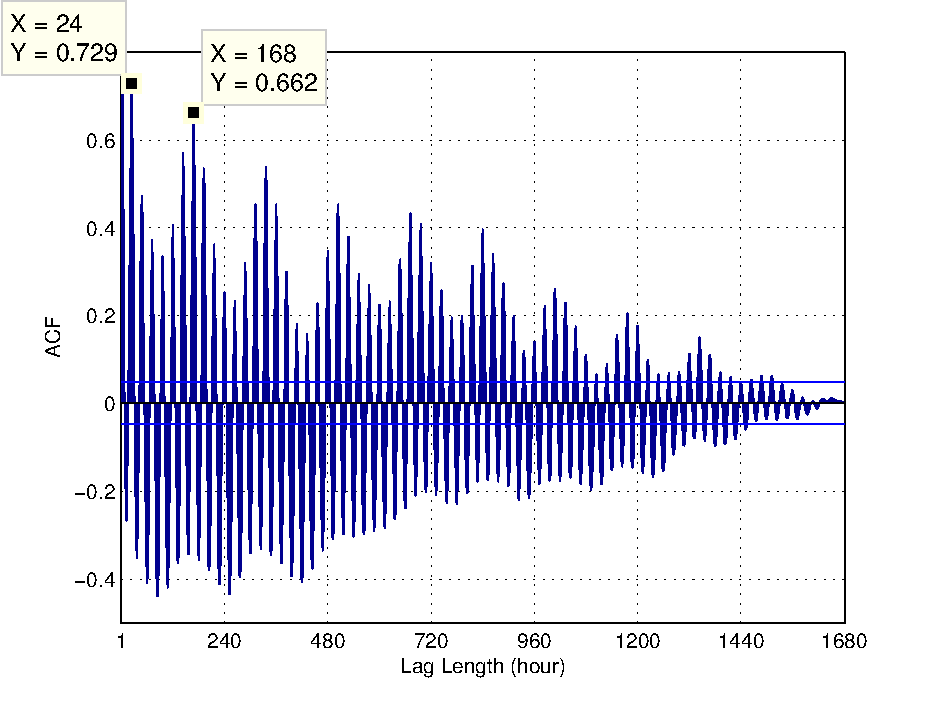
\includegraphics[width=.5\textwidth]{figs/acf_101A1_GHP-eps-converted-to.pdf}
\caption{Auto-correlation of a usual signal from the Building 1 dataset.
The signal features daily and weekly patterns (resp. $x=24$ and $x=168$).}
\label{fig:autocorr}
\end{center}
\end{figure}

An explanation for this is that the daily occupant usage patterns %office hours, 
drive these results.
Figure \ref{fig:diagram1} demonstrates this more clearly.  It shows two 1-week raw signals traces which feature the same 
diurnal pattern.  
This trend is present in almost every sensor trace, and, it hides 
the smaller fluctuations providing more specific patterns driven by local occupant activity.  Upon deeper inspection, we uncovered several
 dominant patterns, common among energy-consuming devices in buildings~\cite{wrinch:pes2012}.  Figure~\ref{fig:autocorr} depicts the 
 auto-correlation of a usual electric power signal for a device.  The two highest values in the figure correspond to a lag of 24 hours and 168 hours (one week).  
 Therefore, the signal has some periodicity and similar (though not equal) values are seen at daily and weekly time scales.
The daily pattern is due to daily office hours and the weekly pattern corresponds to weekdays and weekends.  
%Indeed, thorough inspection of the data reveals that the 
Correlation analysis on \emph{raw} signals cannot be used to determine meaningful 
inter-device relationships because periodic components act as non-stationary trends for high-frequency phenomenon, 
 making the correlation function irrelevant.  %metric is insufficient with raw signals containing the same dominant pattern.
Such trends must be removed in order to make meaningful progress towards our aforementioned goals.  

In the next section we describe SBS.  
We discuss \emph{strip and bind} in section~\ref{methodo:est}, which addresses de-trending and
relationship-discovery.  Then, we describe how we \emph{search} for changes in usage patterns, 
in section~\ref{methodo:ano}, to identify potential savings opportunities.

%One of the major challenges in this work is to discard these patterns and uncover devices intrinsic relationships.
% This difficulty is overcome by the first part of the method (Strip and Bind) presented in Section \ref{methodo:est}.
% Then, the second part of the method (Search) monitors over time the devices relationships and detect abnormal device behavior changes (Section \ref{methodo:ano}).

\subsection{Spatial Verification}
\subsection{Introduction}
The United States leads the world in per-capita energy consumption.
Our electricity use has consistently increased over the last 40 years~\cite{oecd2011} and other parts of the world are rising all 
too rapidly.  With the specter of climate change and the increasing cost of energy, we must explore new
ways for individuals to gain visibility and insight into their energy consumption in order to optimize and reduce it. 
With the increasing penetration of embedded sensors in the environment and
the continued rise in smartphone adoption, we see an opportunity for smartphones to bridge the physical world
to our computational infrastructure and provide an `energy lens' on the physical world.  

We use mobile phones to construct an entity-relationship 
graph of the physical world and combine it with streaming sensor data in order to perform detailed energy-attribution.
We limit the scope of the world to a single building domain.  We have designed and implemented a real-time, mobile energy auditing
application, called the `Energy Lens', that allows us to collect information about 
things throughout the building and how they are related to each other.  For example, computer X is inside 
room Y and connected to meter Z.  Then, we use these relationships to guide our data look-up and analytical
calculations.  For example, the load curve of room Y consists of the sum of all the power traces for loads
inside room Y.  We use the mobile smartphone as the main input tool.  Our work examines \emph{three main challenges} in setting up and 
deploying a real, whole-building infrastructure to support real-time, 
fined grained energy analytics.  

The first challenge is related to tracking and mobility.
The use of mobile phones presents classical, fundamental challenges related to mobility.  Typically, mobility
refers to the phone, as the person carrying it moves from place to place.  However, in the energy-attribution
context, we are also referring to the movement of energy-consuming objects.  Tracking their relationships to spaces 
and people is as important as tracking people.  We describe how we deal with \emph{both moving people and 
moving objects} and show that these historically difficult problems can be addressed relatively easily, if the proper infrastructure is 
in place.  %We provide evidence that the approach is simple, incrementally deployable, and scalable.

The second challenge is about capturing the inter-relationship semantics and having these inform our  analytics.
We adopt the general notion of physical tags that identify objects in the world.  Our system uses \emph{QR codes} to tag things and locations 
in the physical world.  However, \emph{any tag that provides a unqiue identifier for an object could serve the same purpose}.
Once tagged, there are three types of interactions -- 
registration, linking, and scanning -- which establish important relationships.  Registration is the act of creating a virtual object 
to represent a physical one.  Linking captures the relationship between pairs of objects.  Scanning is the act of performing an item-lookup.
Each of these interactions requires a set of swiping gestures.  Linking requires two tag swipes while the other two actions
require a single tag swipe.  Internally, we maintain a \emph{entity-relationship graph (ERG)} of things, people, and locations, that gets
updated through these sets of gestures.

The third challenge is about indoor network connectivity and access.
In order to connect these components, we rely on having `ubiquitous' network connectivity.  However, in practice, network
\emph{availability} is intermittent and our system must deal with the challenges of intermittency.  We discuss how caching
and logging are used to address these challenges.  Moreover, when connectivity is re-established, we must deal with
applying updates to the ERG, as captured by the phone while disconnected.  
% Conflicts can also occur during an update.  For example, the two updates may disagree about which items are attached
% to which meters.  We implement a very simple conflict resolution scheme, described in section~\ref{sec:conflicts}.
% Finally, certain physical-state transitions are represented as a set of updates to the ERG that must be applied 
% atomically.  We implement transactions in the log-replay and transaction manager.
% Our `Energy Lens' system is deployed in a building on our campus.  We discuss
% its architecture and our design choices.  
  
% We also discuss novel strategies for tracking moving people/things and describe how we implement these in our system.  In summary, our work
% makes the following contributions:

% \begin{itemize}
% \item We design and implement a system that captures and combines physical entities, their inter-relationships, and real-time sensor data 
% 		in buildings.% using mobile phones, qr code, and a cloud-based infrastructure.
% \item We observe that certain combinations of swipes give us useful information to set the location of people and things over time.
% 		We codify this observation in our \emph{context-tracker} and use it to maintain consistency between the entity-relationship graph and the 
% 		state of the physical world.  To the best of our knowledge, this is radically different from the approaches in standard 
% 		localization techniques.  However, we argue that it can be used to \emph{enhance} their accuracy and overall performance.
% \item We implement a prefetching algorithm to obtain context-dependent information to both improve performance and
% 		enable disconnected operation.  We also design and implement a log-replay and transaction manager over our data management layer.  We describe how different conflict-resolution policies can be implemented and our rationale for the policies we chose.
% \end{itemize}

% \vspace{0.08in}

% In the next sections we go through a motivating scenario.  We then discuss some related work, followed 
% by the system architecture, evaluation, and future directions.

\subsection{Type Verification}
\subsection{Value Verification}



\section{Functional Verification through Classification and Experimentation}
% \section{Anomaly Detection}


\subsection{Methodology}\label{methodo}

\subsubsection{Strip and Bind} \label{methodo:est}

\begin{figure}[t!]
 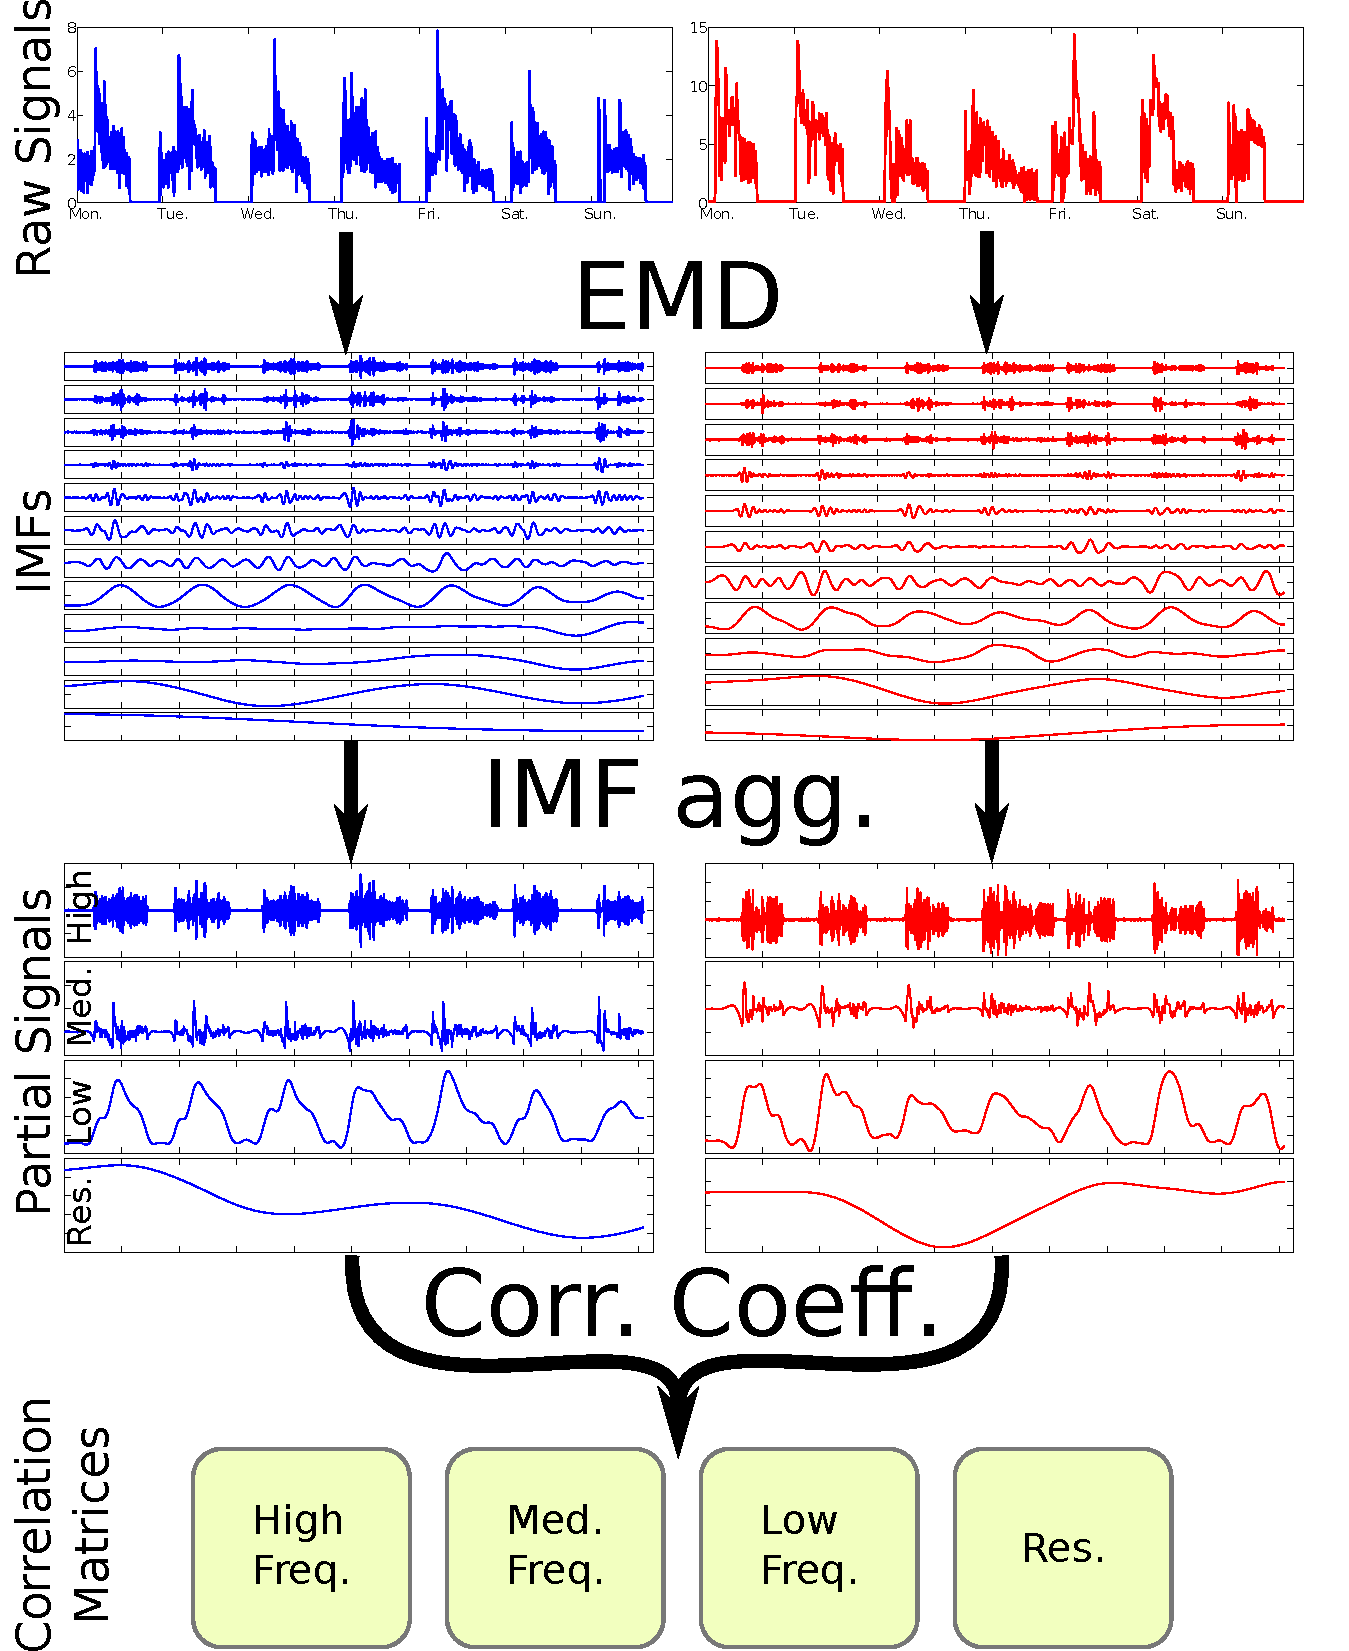
\includegraphics[width=.5\textwidth]{figs/estimator.pdf}
 \caption{\emph{Strip and Bind} using two raw signals standing for one week of data from two different HVACs. (1)~Decomposition of the signals in IMFs using EMD (top to bottom: $c_1$ to $c_n$); (2)~aggregation of the IMFs based on their time scale; (3)~comparison of the partial signals (aggregated IMFs) using correlation coefficient.}
 \label{fig:diagram1}
\end{figure}

%As shown in the previous section, discovering the devices that are used in concert is particularly difficult.
Discovering devices that are used in concert is non-trivial.  
SBS decomposes each signal into an additive set of components, called Intrinsic Mode Functions (IMF), 
that reveals the signal patterns at different frequency bands.  IMFs are obtained using 
%that reveal the signal structures at different time scales.
Empirical Mode Decomposition (see Figure~\ref{fig:diagram1} and Section~\ref{emd}).
%Then, we filter out the IMFs that interfere with our goal and keep only those standing for time scales shorter than the unwanted daily pattern.
%We then remov out IMFs with time scales 
We only consider IMFs with time scales shorter than a day, since we are interested in capturing short-scale usage patterns.
Consequently, SBS aggregates the IMFs that fall into this specific time scale (see \emph{IMF agg.} in Figure \ref{fig:diagram1}).
%The resulting partial signals of different devices are compared pairwise to identify the devices intrinsic relationships (see \emph{Corr. Coeff.} in Figure\ref{fig:diagram1}). 
The resulting partial signals of different device power traces are compared, pairwise, to identify the devices that show un/correlated usage patterns (see \emph{Corr. Coeff.} in Figure~\ref{fig:diagram1}).


% These intrinsic relations are uncovered by comparing the sensors data at certain meaningful frequency bands.
% Namely, looking at high frequency allows to compare short-term variations representing the instantaneous devices change of state, however, the low frequency highlights long-term fluctuations revealing long devices usage pattern.
% 
% ..... the similarity estimators analyzes the readings from several sensors and reports scores standing for the similarity of the sensors at different frequency bands.
% First, the similarity estimator takes advantage of EMD to decompose the sensors signals into a set of components called intrinsic mode functions (IMFs).
% Second, it constructs band-limited signals by aggregating the IMFs whose mean frequencies fall in a certain frequency band.
% Thereby the pairwise comparison of band-limited signals provides the sensors correlations at different frequency bands. 
% 
% The advantages of the proposed intrinsic-correlation estimator are adaptive approach, ... 

% These two steps are described by the two following sections.

\subsubsection{Empirical Mode Decomposition} \label{emd}
Empirical Mode Decomposition (EMD) \cite{huang:emd1998} is a technique that decomposes a signal and reveals intrinsic patterns, 
trends, and noise.
This technique has been widely applied to a variety of datasets, including climate variables~\cite{lee:climateEMD2011}, medical data~\cite{blanco:bioMed2008}, speech signals~\cite{huang:signalProc2006,hasan:ieeeletter2009}, and image processing~\cite{nunes:vision2005}.
% for example, it helped to uncover the global surface temperature trends\cite{}, solar activity patterns and predicts climate variables .
EMD's effectiveness relies on its empirical, adaptive and intuitive approach.
In fact, this technique is designed to efficiently decompose both non-stationary and non-linear signals without requiring any 
a priori basis functions or tuning.  

EMD decomposes a signal into a set of oscillatory components called intrinsic mode functions (IMFs). 
An IMF satisfies two conditions: (1) it contains the same number of extrema and zero crossings (or differ at most by one); (2) the two 
IMF envelopes defined by its local maxima and local minima are symmetric with respect to zero.  Consequently, 
 IMFs are functions that directly convey the amplitude and frequency modulations.

% EMD is an iterative sifting process that extracts IMFs step by step; each step seeks for the IMF with the highest frequency, then the computed IMF is removed from the data and the residual data are used as input for the next step.
EMD is an iterative algorithm that extracts IMFs step by step by using the so-called sifting process \cite{huang:emd1998}; each step seeks for the IMF with the highest frequency by sifting, then the computed IMF is removed from the data and the residual data are used as input for the 
next step.
The process stops when the residual data becomes a monotonic function from which no more IMF can be extracted.

We formally describe the EMD algorithm as follows: 
\begin{enumerate}
\item Sifting process: For a current signal $h_0=X$, let $m_0$ be the mean of its upper and lower envelopes as determined from a cubic-spline interpolation of local maxima and minima.
\item The estimated local mean $m_0$ is removed from the signal, giving a first component: $h_1 = h_0-m_0$
\item The sifting process is iterated, $h_1$ taking the place of $h_0$. Using its upper and lower envelopes, a new local mean $m_1$ is computed and $h_2 = h_1-m_1$.
\item The procedure is repeated $k$ times until $h_k=h_{k-1}-m_{k-1}$ is an IMF according to the two conditions above.
\item This first IMF is designated as $c_1 = h_k$, and contains the component with shortest periods. We extract it from the signal to produce a residual: $r_1 = X - c_1$.  Steps 1 to 4 are repeated on the residual signal $r_1$, providing IMFs $c_j$ and residuals $r_j  = r_{j-1}-c_j$, for $j$ from $1$ to $n$.
\item The process stops when residual $r_n$ contains no more than 3 extrema.
\end{enumerate}

The result of EMD is a set of IMFs $c_i$ and the final residue $r_n$, such as: \[X=\sum^{n}_{i=1}c_i+r_n\]
where the size of the resulting set of IMFs ($n$) depends on the original signal $X$ and $r_n$ represents the trend of 
the data (see \emph{IMFs} in Figure~\ref{fig:diagram1}).

For this work we implemented a variant of EMD called Complete Ensemble EMD~\cite{torres:icassp2012}.
This algorithm computes EMD several times with additional noise, it allows us to efficiently analyze signals that have 
flat sections (i.e. consuming no electricity in our case). % and permits us to solve the \emph{EMD mode mixing problem}.

\subsubsection{IMF aggregation} \label{methodo:corr}
By applying EMD to energy consumption signals we obtain a set of IMFs that precisely describe the devices consumption 
patterns at different frequency bands.  Therefore, we can focus our analysis on the smaller time scales, ignoring the dominant 
patterns that prevent us from effectively analyzing raw signals.

However, comparing the IMFs obtained from different signals is also not trivial,
 because EMD is empirically uncovering IMFs from the data there is no guarantee that the two IMFs $c_i^1$ and $c_i^2$ obtained from two distinct signals $S^1$ and $S^2$ represent data at the same frequency domain.
Directly comparing $c_i^1$ and $c_i^2$ is meaningless unless we confirm that they belong to the same frequency domain.

There are numerous techniques to retrieve IMF frequencies~\cite{huang:aada2009}.  
In this work we take advantage of the Generalized Zero Crossing (GZC)~\cite{huang:patent2006} because it is a simple and robust 
estimator of the instantaneous IMF frequency \cite{huang:aada2009}.
GZC is a direct estimation of IMF instantaneous frequency using critical points defined as the zero crossings and local extrema 
(round dots in Figure~\ref{fig:gzc}).
Formally, given a data point $p$, GZC measures the quarter ($T_4$), the two halves ($T_2^x$), and the four full periods ($T_1^y$), $p$   
belong to (see Figure~\ref{fig:gzc}) and the instantaneous period is computed as:
\[T=\frac{1}{7}\{4T_4+(2T_2^1+2T_2^2)+(T_1^1+T_1^2+T_1^3+T_1^4)\}\]

\begin{figure}
\begin{center}
 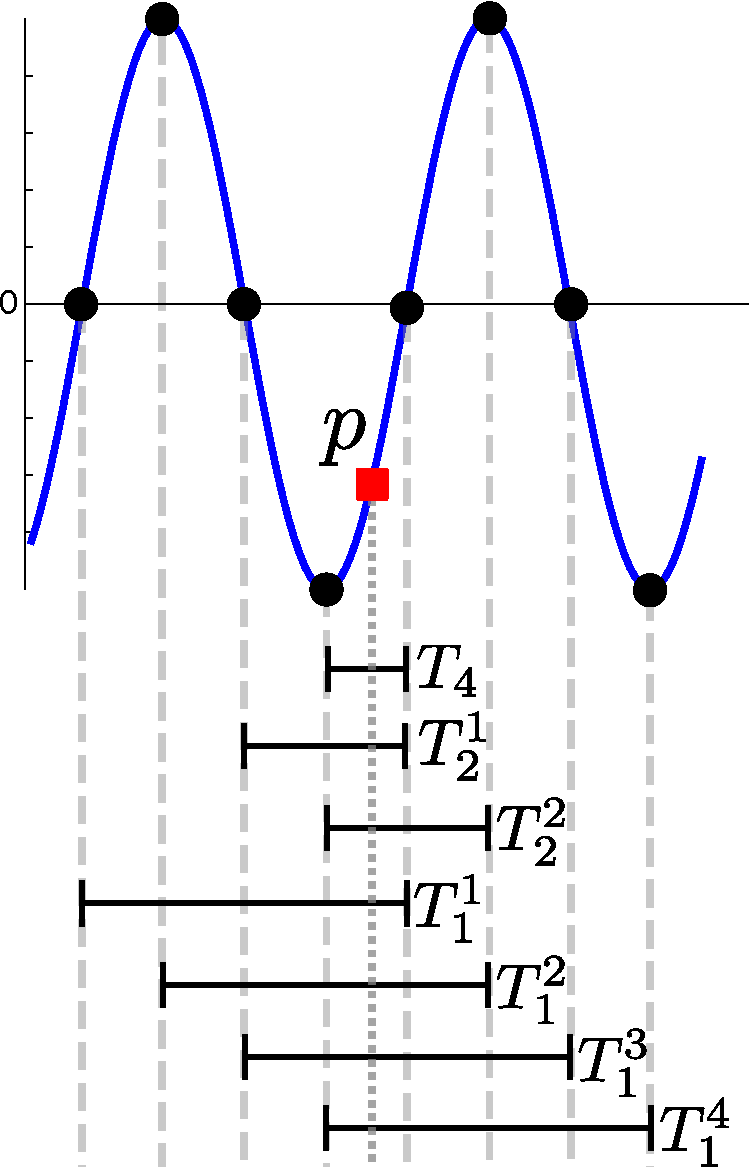
\includegraphics[width=.25\textwidth]{figs/gzc.pdf}
 \end{center}
 \caption{Generalized Zero Crossing: the local mean period at the point $p$ is computed from one quarter period $T_4$, two half periods $T_2^x$ and four full periods $T_1^y$ (where $x=1, 2$, and, $y=1,2,3,4$).}
 \label{fig:gzc}
\end{figure}

Since all points $p$ between two critical points have the same instantaneous period GZC is local down to a quarter period.
Hereafter, we refer to the time scale of an IMF as the average of the instantaneous periods along the whole IMF.
Because the time scale of each IMF depends on the original signal, we propose the following to efficiently compare IMFs from different signals.
We cluster IMFs with respect to their time scales and partially reconstruct each signal by aggregating its IMFs from the 
same cluster.  Then, we directly compare the partial signals of different devices.

The IMFs are clustered using four time scale ranges: 
\begin{itemize}
 \item The \emph{high frequencies} are all the IMFs with a time scale lower than 20 minutes. These IMFs capture the noise.
 \item The \emph{medium frequencies} are all the IMFs with a time scale between 20 minutes and 6 hours. These IMFs convey the detailed devices usage.
 \item The \emph{low frequencies} are all the IMFs with a time scale between 6 hours and 6 days. These IMFs represent daily device patterns.
 \item The \emph{residual data} is all data with a time scale higher than 6 days. This is mainly residual data obtained after applying EMD.  Also, it highlights the main device trend.
\end{itemize}

These time scale ranges are chosen based on our experiments and goal.
The 20-minute boundary relies on the sampling period of our dataset (5 minutes) and permits us to capture IMFs with really short periods.
The 6-hour boundary allows us to analyze all patterns that have a period shorter than the usual office hours.
The 6-day boundary allows us to capture daily patterns and weekday patterns.

Aggregating IMFs, within each time scale range, results in 4 partial signals representing different characteristics of the device's
 energy consumption (see \emph{Partial Signals} in Figure~\ref{fig:diagram1}).
We do a pairwise device trace comparison, calculating the correlation coefficient of their partial signals.
In the example shown in Figure~\ref{fig:diagram1}, the correlation coefficient of the raw signals suggests that they are highly correlated ($0.57$). 
However, the comparison of the corresponding \emph{partial signals} provides new insights;
the two devices are poorly correlated at high and medium frequencies (respectively $-0.01$ and $-0.04$) but highly correlated at low frequencies ($0.79$) meaning that these devices are not ``intrinsically'' correlated.  They only share a similar daily pattern.

All the devices are compared pairwise at the four different time scale ranges.
Consequently, we obtain four correlation matrices that convey device similarities at different time scales.
Each line of these matrices (or column, since the matrices are symmetric) reveals the behavior of a device -- its relationships with the 
other devices at a particular time scale.
The matrices form the basis for tracking the behavior of devices and to search for misbehavior.


\subsubsection{Search}\label{methodo:ano}
\emph{Search} aims at identifying misbehaving devices in an unsupervised manner.
Device behavior is monitored via the correlation matrices presented in the previous section.
Using numerous observations SBS computes a specific reference that exhibits the normal inter-device usage pattern.
Then, SBS compares the computed reference with the current data and reports devices that deviate from their usual 
behavior.

\subsubsection{Reference}
We define four reference matrices, which capture normal device behavior at the four time scale ranges defined in 
Section~\ref{methodo:corr}.
The references are computed as follows: (1) we retrieve the correlation matrices for $n$ consecutive time bins. (2) For each pair of devices we compute the median correlation 
over the $n$ time bins and obtain a matrix of the median device correlations.

Formally, for each time scale range the computed reference matrix for $d$ devices and $n$ time bins is:
\[R_{i,j} =  \median(C^1_{i,j},...,C^n_{i,j})\]
where $i$ and $j$ ranges in $[1,d]$.

% Assuming that device-usage predominantly behaves normally and the anomalies are exceptional 
% events, the reference matrices exhibit the normal device behaviors.
% Our model assumes anomalies are rare and the majority of the data is normal.
% This is a common assumption in unsupervised anomaly detection.
Because anomalies are rare by definition, we assume the data used to construct the reference matrix
is an accurate sample of the population; it is unbiased and accurately captures the range of normal behavior.
% We assume that normal behavior is not truly anomalous.
Abnormal correlation values, that could appear during model construction, %in the analyzed time bins 
are ignored by the median operator thanks to its robustness to outlier (50\% breakdown point).  
However, if that assumption does not hold (more than 50\% of the data is anomalous), our model will flag the opposite -- labeling abnormal as normal and vice-versa.
From close inspection of our data, we believe our primary assumption is sound.
% Normal behavior occurs most frequently, therefore detected anomalies should be meaningful.



\subsubsection{Behavior change}
% SBS consists in identifying the devices that significantly deviate from their normal behaviors as defined in the reference matrices.
% Consequently, 
We compare each device behavior, for all time bins, to the one provided by the reference matrix.  
Consider the correlation matrix $C^t$ obtained from the data for time bin $t$ ($1 \leq t \leq n$).  
Vector $C^t_{i,*}$ is the behavior of the $i^{th}$ device for this time bin.
Its normal behavior is given by the corresponding vector in the reference matrix $R_{i,*}$.
We measure the device behavior change at the time bin $t$ with the following Minkowski weighted distance:
\[ l^t_{i} = \left(\sum_{j=1}^d  w_{ij}\left(C^t_{i,j} - R_{i,j}\right)^p\right)^{1/p} \]
where $d$ is the number of devices and $w_{ij}$ is:
\[ w_{ij} = \frac{R_{i,j}}{\sum_{k=1}^d R_{i,k}}. \]
The weight $w$ enables us to highlight the relationship changes between the device $i$ and those highly correlated to it in the reference matrix.
In other words, our definition of behavior change is mainly driven by the relationship among devices that are usually used in concert.
We also set $p=4$ in order to inhibit small differences between $C^t_{i,j}$ and $R_{i,j}$ but emphasize the important ones.

By monitoring this quantity over several time bins the abnormal device behaviors are easily identified as the outlier values.
In order to identify these outlier values we implement a robust detector based on median absolute deviation (MAD), a dispersion measure commonly used in anomaly detection \cite{huber:wiley2009,chan:springer2005}.
It is a measure that robustly estimates the variability of the data by computing the median of the absolute deviations from the median of the data.
 Let $l_{i} = [l_i^1,...,l_i^n]$ be a vector representing the behavior changes of device $i$ over $n$ time bins, then its MAD value is defined as:
\[ \mad_i = b \median(\lvert l_{i} - \median(l_{i})\rvert)\]
where the constant $b$ is usually set to $1.4826$ for consistency with the usual parameter $\sigma$ for Gaussian distributions.
Consequently, we define anomalous behavior, for device $i$ at time $t$, such that the following equation is satisfied:%of the device $i$ at the time bin $t$ that satisfies the following equation:
\[l^t_{i} > \median(l_{i}) + \tau  \mad_i\]
Note, $\tau$ is a parameter that permits to make SBS more or less sensitive.

The final output of SBS is a list of alarms in the form $(t,i)$ meaning that the device $i$ has abnormal behavior at the time bin $t$.
The priority of the alarms in this list is selected by the building administrator by tuning the parameter $\tau$.

\section{Dataset}
The data we used was obtained from a deployment of sensors in a 12-story office building
on the campus of the University of Tokyo~\cite{gutp, ogawa:lncs2011}.  The deployment consists of 
almost 700 sensors monitoring device power consumption, ranging from plug-load devices to components of the
heating, ventilation, and air conditioning system (HVAC) and lighting.  Sensors also reported temperature, 
pressure, device-state, and other information.  Each sensor reports data on the
order of minutes.  Over 500 GBs of data was collected over a 2-year span.

\begin{figure*}[tb]
\hspace{-2cm}
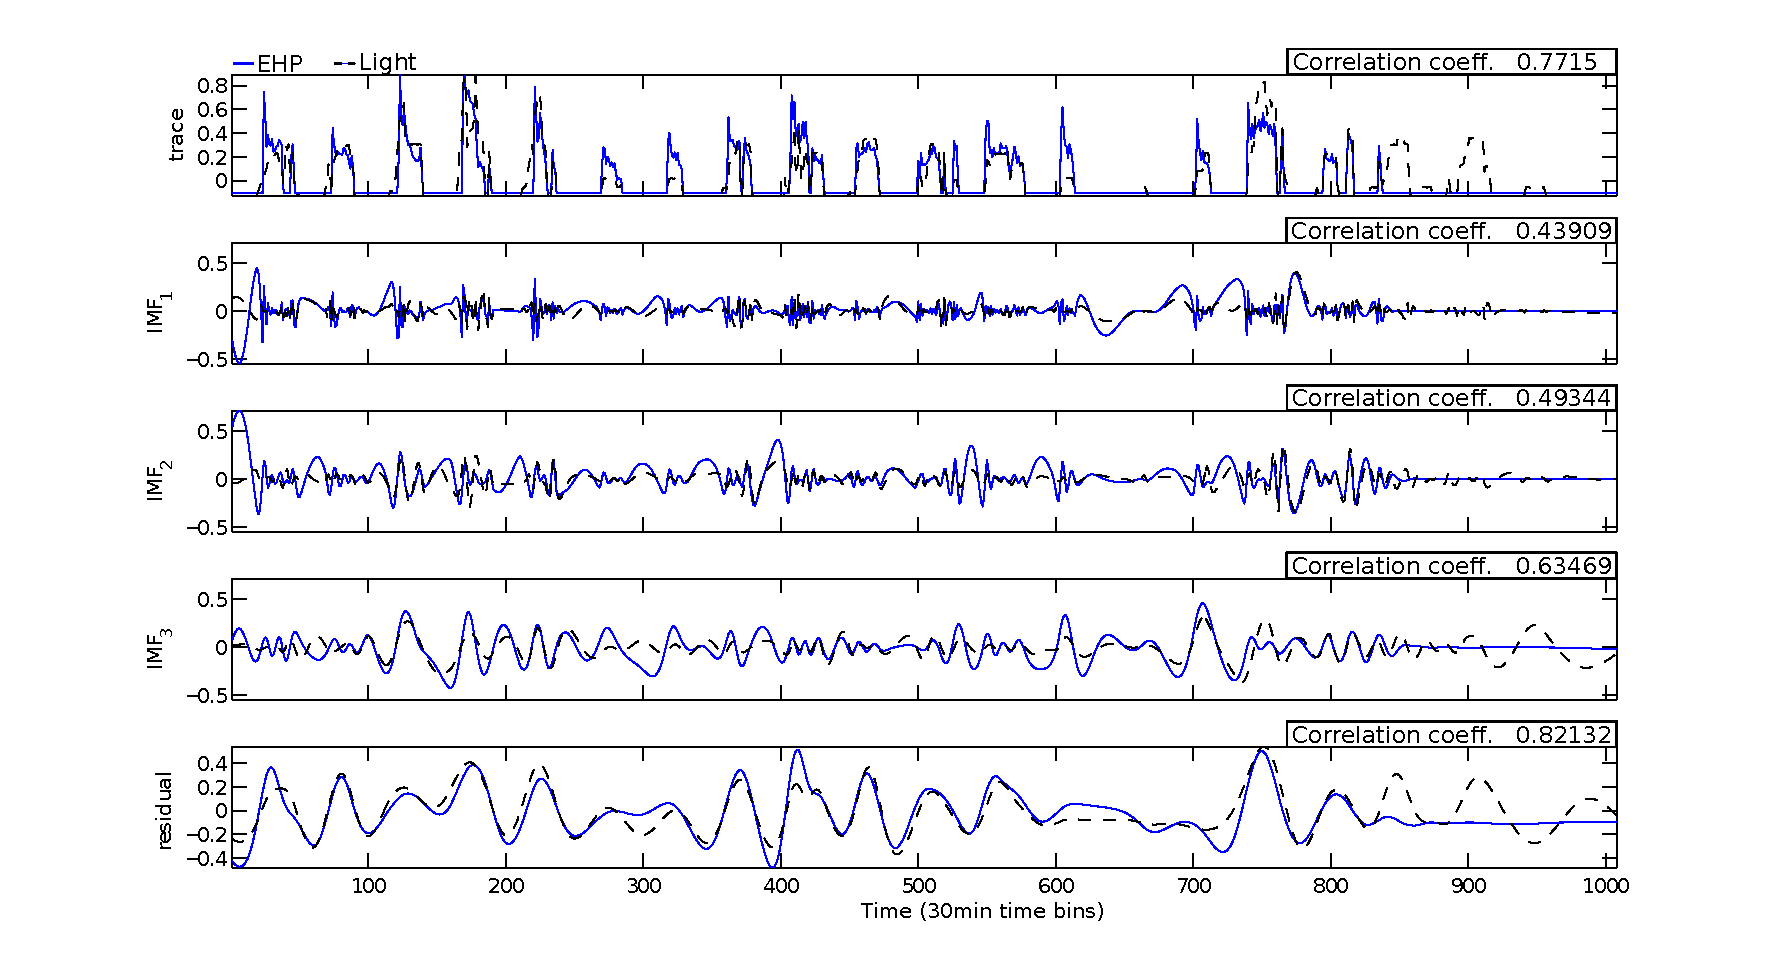
\includegraphics[width=1.2\textwidth]{img/emd_25_26-eps-converted-to}
\vspace{-1cm}
\caption{Decomposition of the EHP and light trace using bivariate EMD. IMFs correlation coefficients highlight the intrinsic relationship of the two traces.}
\label{fig:emd}
\end{figure*}

% The intent of the Green University of Tokyo Project (GUTP) \cite{gutp} is to reduce the university environmental impacts associated to its electric energy consumption.
% The first step of this project was to deploy sensors at the Building No.2 of the Faculty of Engineering 
% Electric power consumption of a 12 floors building containing researchers office and classroom.
% 1215 sensors monitoring different devices...

%received attention in the past \cite{ogawa:lncs2011}.

For this investigation, we focus on a three-week span in the summer of 2011 (from July 4th to July 24th).
The dataset captures regular work days, weekends, and one holiday (July 18th).  This timeframe captures
the typical usage of the equipment, triggered by occupant activity.  For the initial
analysis, we focus on three sensors; two water pumps and a light feed.  The first pump is an 
``electric heat pump'' and is labled as EHP, the second  is a ``gas heat pump''
and labeled as GHP.  The room lighting system serves the same room as the EHP.  The GHP
serve a different room on the same floor.  The expanded portion of our analysis pivots as the EHP
and does a pairwise comparison between it and all other sensors in the building.

% includes one day holiday (July 18th)
% 3 different sensors:
% \begin{itemize}
%  \item Two are measuring the electric power consumption of two devices from the same room; an electric heat 
%  		pump (EHP) and the room lighting system.
%  \item One is measuring the electric power consumption of a gas heat pump (GHP) that is pumping water to cool 
%  		a different room in the same building.
% \end{itemize}

% Later we expand our analysis to include all the sensors in the building.


\section{Problem statement and Initial approach}\label{problem}
% In our analysis, we are focused on finding devices that are correlated in their use over time.  Therefore, the
% main objective is to examine how device traces relate to one another.  The wish to identify
% correlated device-trace patterns at large spatio-temporal scales.

In buildings, metadata is poorly and unsystematically managed within a single system domain.  Moreover, 
with the ever growing number of additional sub-meters, it is important to quickly integrate
sensor data from multiple systems to understand the full state of the building.  It is also important to 
understand how sensors are used in concert.  Anamolies in usage may indicate underlying problems with 
the equipment or inefficient/incorrect usage.  

We begin our analysis by running direct correlation between the traces.
Figure \ref{fig:raw} shows the raw traces for the three devices discussed in 
the previous section (EHP, GHP, light).  All three exhibit a diurnal usage pattern.  On weekends, each
draw less power.  The correlation coefficient for 
 the EHP and light is $0.7715$ and the correlation coefficient for the EHP and GHP is $0.6370$.
Running correlation across them yields high correlation coefficients, mostly
due to their underlying daily usage pattern.

% Usual measures on sensor data like correlation coefficient or granger causality \cite{kim:buildsys2010}
% -- this is not working

\begin{figure}[t!]
\centering
 \subfigure[EHP trace]{\label{fig:raw_ehp}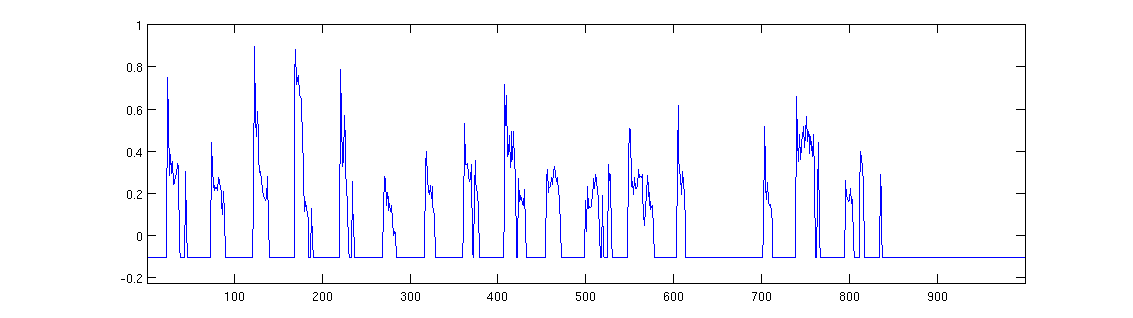
\includegraphics[width=.4\textwidth]{img/25.png}}
 \subfigure[Light trace]{\label{fig:raw_light}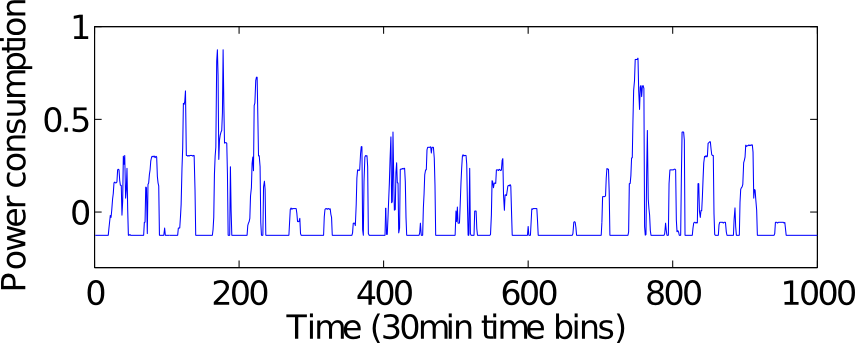
\includegraphics[width=.4\textwidth]{img/26.png}}
 \subfigure[GHP trace]{\label{fig:raw_ghp}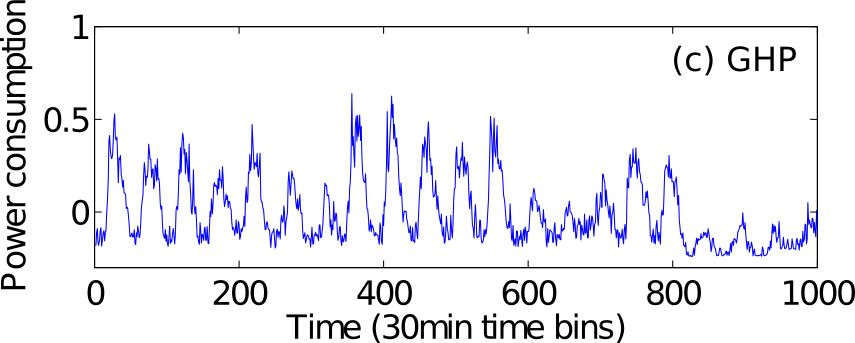
\includegraphics[width=.4\textwidth]{img/41.png}}
 \caption{Traces from three different sensors captured in 2011 from July 4th to July 24th. Data is normalized and aggregated into 30 minutes time bins.}
 \label{fig:raw}
\end{figure}

% For example correlation coefficients for the 3 signals...
% correlation coefficient for the EHP and Light signals: $0.772013$
% correlation coefficient for the EHP and GHP signals: $0.636967$

% These scores suggest that the EHP signal is related to the two other measured signals.

% These results were expected for the EHP and light traces, as the two measured devices operate for the same room 
% and are used simultaneously.  More importantly, they are used to support the occupants of the rooms they are serving.
% We were somewhat surprised by the magnitude of correlation between the pumps, since they serve rooms on
% opposite sides of the building and operate independently.  However, occupancy and weather patterns are similar,
% and the underlying trend is captured by the correlation calculation.
% The difference between the correlation coefficients is small and one might conclude that all three are
% closely related to one another.  That conclusion is not false but misleading.  Correlation on the raw 
% traces is sensitive to the underlying trend shared by the traces.  In order to meaningfully distinguish between
% truly related devices we need to remove the common trends. 

Our initial results were not surprising.  The diurnal pattern dominates the comparison between the sensors.
Weather is the main driver for this behavior and it affects the readings in almost all of the
sensors in our dataset.  Cross-correlation on raw sensor data is insufficient for filtering intrinsically related
behavior.  Upon closer examination of the data we assess the following:

\begin{itemize}
\item The main underlying diurnal trend occurs in almost all the traces.
\item Occupancy and room activities occur at random times during the day and change 
		at a higher frequency than weather patterns.
\item Sensors that serve the same location observe the same activities.  Therefore, their underlying
		measurements should be correlated.
\end{itemize}

In order to uncover these relationships we must remove low-frequency trends in the traces and
compare the readings at high frequencies.

% \begin{table}
% \begin{center}
% \begin{tabular}{|l|l|l|l|l|l|}
% \hline
% × & Raw trace & 1st IMF & 2nd IMF & 3rd IMF & Residual\\ \hline
% EHP, Light & 0.7715 & 0.43909 & 0.49344 & 0.63469 & 0.82132 \\ \hline
% EHP, GHP & 0.6370 & 0.0060274 & 0.063546 & 0.16764 & 0.79378 \\ \hline
% \end{tabular}
% \caption{Correlation coefficients of the analyzed trace and their IMFs uncovered by EMD}
% \label{tab:corr}
% \end{center}
% \end{table}
% \subsection{Simple Scenario}

\begin{figure*}[tb]
\hspace{-2cm}
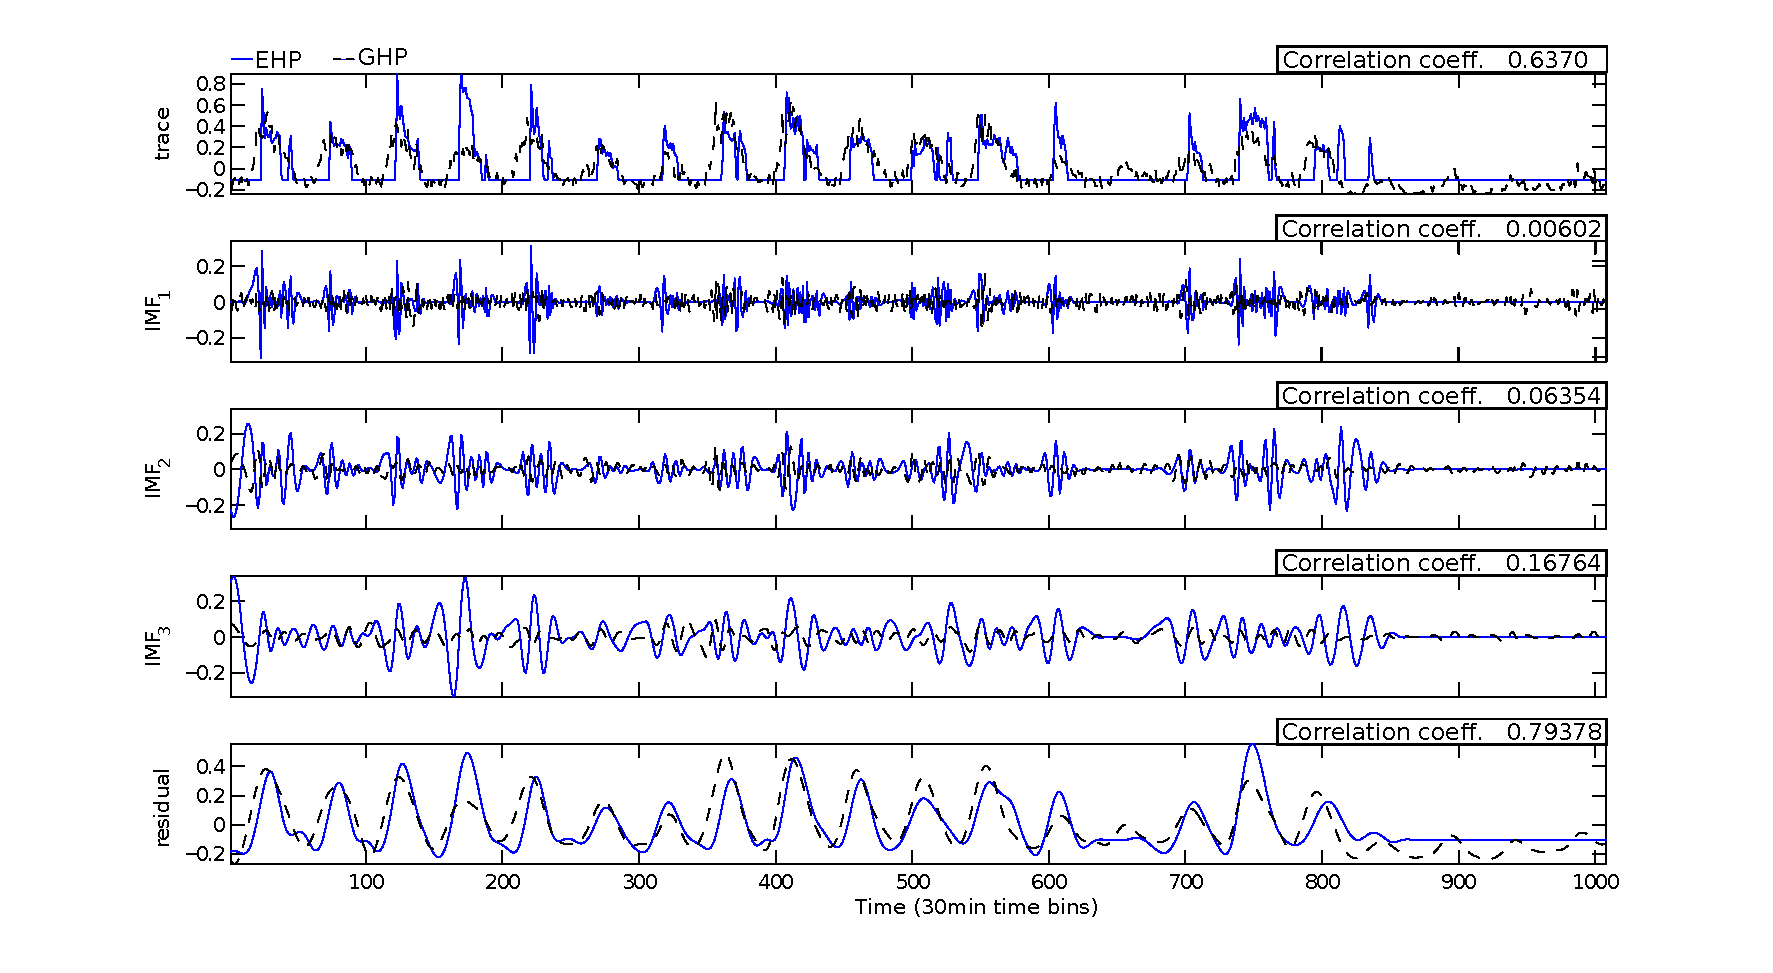
\includegraphics[width=1.2\textwidth]{img/emd_25_41-eps-converted-to}
\vspace{-1cm}
\caption{Decomposition of the EHP and GHP trace using bivariate EMD. IMFs correlation coefficients highlight the intrinsic independence of the two traces.}
\label{fig:emd2}
\end{figure*}

% The small difference between the two computed correlation coefficients is misleading as one could conclude that the three signals are correlated and the corresponding devices are activated by a single action.

% The high correlation coefficients obtained for these three signals result .... weekly pattern....
% small difference = local fluctuation...

% this high score comes from the fact that the two devices are monitoring offices that are weekly used.

% Indeed the weekly pattern of the data trump the correlation coefficients....

% How to inspect only the local fluctuations...?
% we'd like to have an elegant solution (i.e. not specifying the interesting time scale)


\begin{figure*}[t!]
% \subfloat[Raw signals]{\includegraphics[width=.48\textwidth]{img/heatMap_raw_201106-eps-converted-to.pdf}}\\
\subfloat[High Frequencies\label{fig:heatmap:high}]{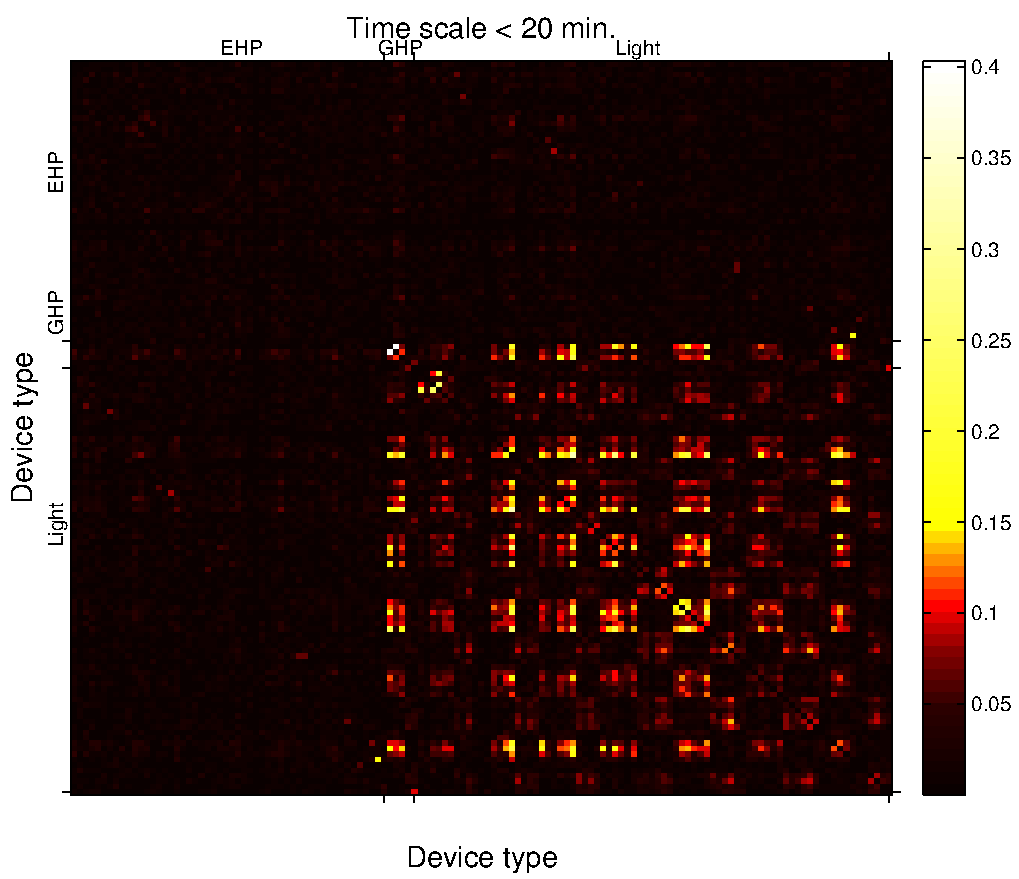
\includegraphics[width=.48\textwidth]{figs/heatMap_1_201106-eps-converted-to.pdf}}\hfill
\subfloat[Medium Frequencies\label{fig:heatmap:med}]{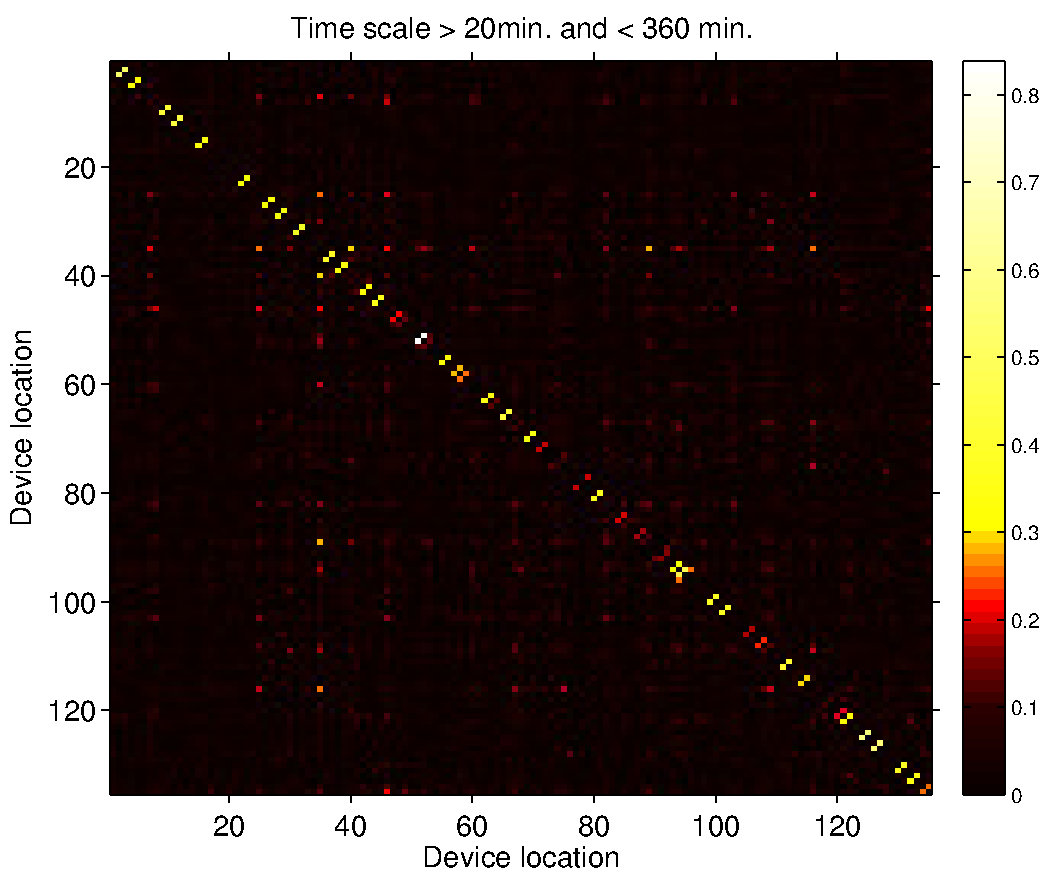
\includegraphics[width=.48\textwidth]{figs/heatMap_2_201106-eps-converted-to.pdf}}\\
\subfloat[Low Frequencies\label{fig:heatmap:low}]{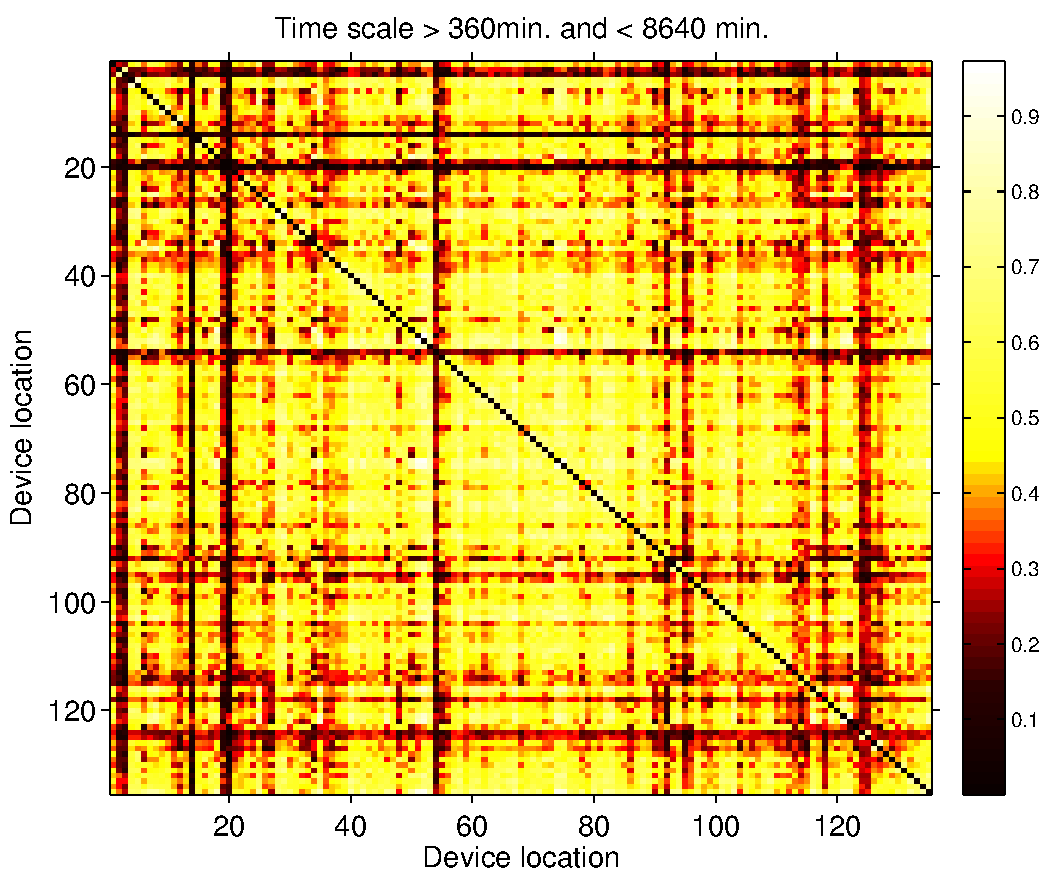
\includegraphics[width=.48\textwidth]{figs/heatMap_3_201106-eps-converted-to.pdf}}\hfill
\subfloat[Residual data\label{fig:heatmap:res}]{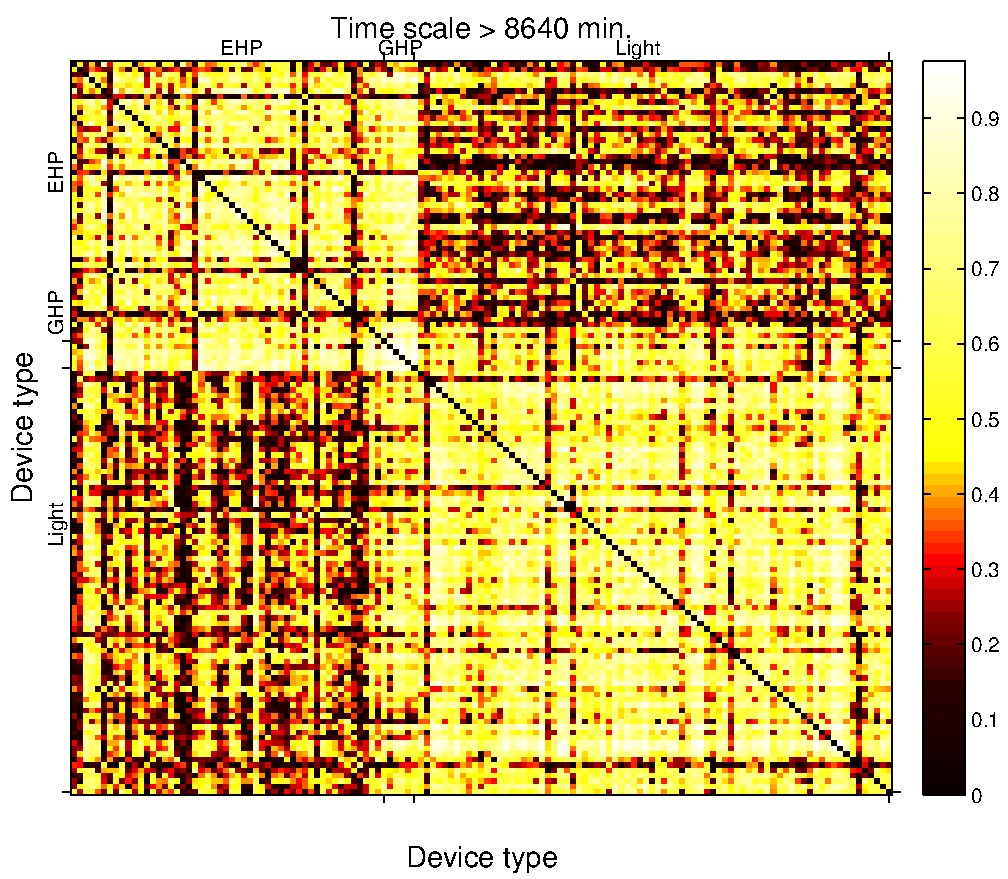
\includegraphics[width=.48\textwidth]{figs/heatMap_4_201106-eps-converted-to.pdf}}
\caption{Reference matrices for the four time scale ranges (the diagonal $x=y$ is colored in black for better reading). The medium frequencies highlight devices that are located next to each other thus intrinsically related. The low frequencies contains the common daily pattern of the data. The residual data permits to visually identify devices of the similar type.}
\label{fig:heatmap}
\end{figure*}

\section{Function Verification: Experimental Results}
\label{eval}
In this section we evaluate SBS on our building traces.  We demonstrate
 the benefits of striping the data by monitoring patterns captured at different time scales.
Then, we thoroughly investigate the alarms reported by SBS.  

\subsubsection{Shortcomings}
Because our analysis is done on historical data, some of the faults found by SBS could not be fully
corroborated.  In order to fully examine the effectiveness of our approach, we must run it in real time and
physically check that the problem is actually occurring.  When a problem is detected
in the historical trace, months after it has occurred, the current state of the building may no longer reflect
what is in the traces.  Some of the anomalies discussed in this section uncover interpretable patterns 
that are difficult to find in practice.  For example, simultaneous heating and cooling is a known, recurring problem
 in buildings, but it is very hard to identify  when it is occurring.  Some of the anomalies we could not interpret
might be interpretable by a building manager, however, we did not consult either building manager for this study.
Therefore, the results of this study do not examine the true/false positive rate exhaustively.

The true/false negative rate is impractical to assess.  It may be examined through synthetic stimulation of
the building via the control system.  However, getting cooperation from a building manager to hand over control of the building
for experimentation in non-trivial.  Therefore, we forgo a full true/false negative analysis in our evaluation.

Because of these challenges, the evaluation of SBS focuses on comparing the output with known fault
signatures.  We examine anomalies, in either building, where the anomaly is easily interpretable but
difficult to find by the building manager.  We forego a comparison of SBS with competing algorithms because
 related algorithms require detailed knowledge of the building, \emph{a priori}.  The advantage of SBS is that it 
requires no such information to provide immediate value.

\subsubsection{Device behavior at different time scales}
The Strip and Bind part of SBS is evaluated using the data from Eng. Bldg 2. %, since we can verify how items are being used and use it as ground truth.
This dataset is appropriate to measure SBS's performance, since lighting and HVAC systems serving the same room are usually used 
simultaneously.
Consequently, we analyze this data using SBS and verify that the higher correlations at medium frequencies correspond to devices located in the same room. % and the unwanted data is captured at the other frequencies.

The dataset is split into 10, one-week bins and each bin is processed by SBS.
Using the 10 correlation matrices at each time scale range, SBS uncovers the four reference matrices depicted in 
Figure~\ref{fig:heatmap}.

\paragraph{High frequencies}
In this work the high frequencies correspond to the signals \emph{noise}, 
therefore, we do not expect any useful information from the corresponding matrix (Figure \ref{fig:heatmap:high}).
Indeed, the corresponding reference matrix does not provide any help to determine a device's relative location.
Thus, we emphasize that high frequency data should be ignored for uncovering device relationships (in contrast to \cite{romain:iotapp12}).
Interestingly, we find that the sensors monitoring the lights generate consistent noise. % and could help one to cluster this type of sensor.
  
\paragraph{Medium frequencies}
Our main focus is on the medium frequencies as it is designed to capture the intrinsic device relationships.
Figure \ref{fig:heatmap:med} shows the correlation matrix at medium frequencies.
It is significantly different from the one obtained with the raw signals (Figure \ref{fig:heatmap:raw}): high correlation coefficients are concentrated along the matrix diagonal. 
Since devices serving the same or adjacent rooms are placed nearby in the matrix it validates our hypothesis: \emph{high correlation scores within the medium frequency band shows strong inter-device relationships}.

Considering this reference matrix as an adjacency matrix of a graph, in which the nodes are the devices, we identify the clusters of 
correlated devices using a community mining algorithm~\cite{blondel:unfolding}.
As expected we obtain mainly clusters of only two devices (light and HVAC serving the same room), but we also find clusters that are composed of more devices.
For example a cluster contains 3 HVAC systems serving the three server rooms. Although these server rooms are located on
 different floors, SBS shows a strong correlation between these devices.  Coincidentally, they are managed similarly.
Interestingly, we also observe a couple of clusters that consist of independent devices serving adjacent rooms belonging to the same lab.
The bigger cluster contains 33 devices that are 2 GHP devices and the corresponding lights.
This correlation matrix and the corresponding clusters 
highlight the ability for SBS to identify such hidden inter-device usage relationships.
 
\paragraph{Low frequencies}
Low frequencies capture daily patterns, embedded in all the device traces.  
Figure \ref{fig:heatmap:low} depicts the corresponding reference matrix which is similar to the one of raw signal traces (Figure \ref{fig:heatmap:raw}) 
and it shows no particular structure.% (daily patterns account for the coefficients high values).  
% Since this matrix contains mainly high values, most of the partial signals at low frequencies features similar characteristics (i.e. daily patterns).
These partial signals are discarded as they do not help us in identifying inter-device usage patterns.
 
\paragraph{Residual data}
The residual data shows the weekly trend, which gives us no information about device relationships.
But, surprisingly, by reordering the correlation matrix based on the type of the devices (Figure \ref{fig:heatmap:res}) 
we can visually identify two major clusters.
The first cluster consists of HVAC devices (see EHP and GHP in Figure \ref{fig:heatmap:res}) and the second one contains only lights. 
An in-depth examination of the data reveals that long-term trends are inherent to the device types. 
For example, as the consumption of both the EHP and GHP devices is driven by the building occupancy and the outside temperature, these two types of devices follow the same trend. 
However, the use of light is independent from the outside temperature thus the lighting systems follow a common trend different from the EHP and GHP one.

We conduct the same experiments by splitting the dataset in 70 bins of 1 day long and observe analogous results at high and medium frequencies but not at lower frequencies.  This is because the bins are too short to exhibit daily oscillations and the residual data captures only the daily trend.

% TODO add some info about the reference matrix for the Building 2?

\subsubsection{Anomalies}
We evaluate the \emph{search} performance of SBS using the traces from the Eng. Bldg 2 and Cory Hall.
%% Romain
Due to the lack of historical data, such as room schedule or reports of energy waste, the evaluation is non-trivial.
Furthermore, getting ground truth data from a manual inspection of the hundreds traces of our data sets is impractical.
The lack of ground truth data prevents us from producing a systematic analysis of the anomalies missed by SBS (i.e. false negatives rate).
Nevertheless, we exhibit the relevance of the anomalies uncovered by SBS (i.e. high true positive rate and low false positive rate) by manually checking the output of SBS.
%% Romain

\paragraph{Anomaly classification}
To validate SBS results we manually inspect the anomalies detected by the algorithm.  
For each reported alarm $(t,i)$ we investigate the device trace $i$ and the devices correlated to it
to determine the reason for the alarm.
Specifically, we retrieve the major relationship change that causes the alarm (i.e. $\max(|w_j(C_{i,j}^t - R_{i,j})|)$, 
see Section \ref{methodo:ano}) and examine the metadata associated to the corresponding device.
% $j$ and the sign of the relationship change $C_{i,j}^t - R_{i,j}$.
% A positive value of relation change means the devices correlation at the time bin $t$ is abnormally high, whereas negative value means that the relationship between the two devices is broken.
This investigation allows us to classify the alarms into five groups:
\begin{itemize}
 \item \emph{High power usage}: alarms corresponding to electricity waste.
 \item \emph{Low power usage}: alarms representing the abnormally low electricity consumption of a device.
 \item \emph{Punctual abnormal usage}: alarms standing for short term (less than 2.5 hours) raise or drop of the electricity consumption.
 \item \emph{Missing data}: alarms raised due to a sensor failure.
 \item \emph{Other}: alarms whose root cause is unclear.
\end{itemize}

% However, the exhaustive enumeration of the true negatives (i.e. saving opportunities that are not detected) is impractical because of the size of the analyzed datasets (number of devices and traces length).
% Instead we exhibit the detector sensitivity by varying $\tau$, the threshold value.

\begin{figure}
\begin{center}
 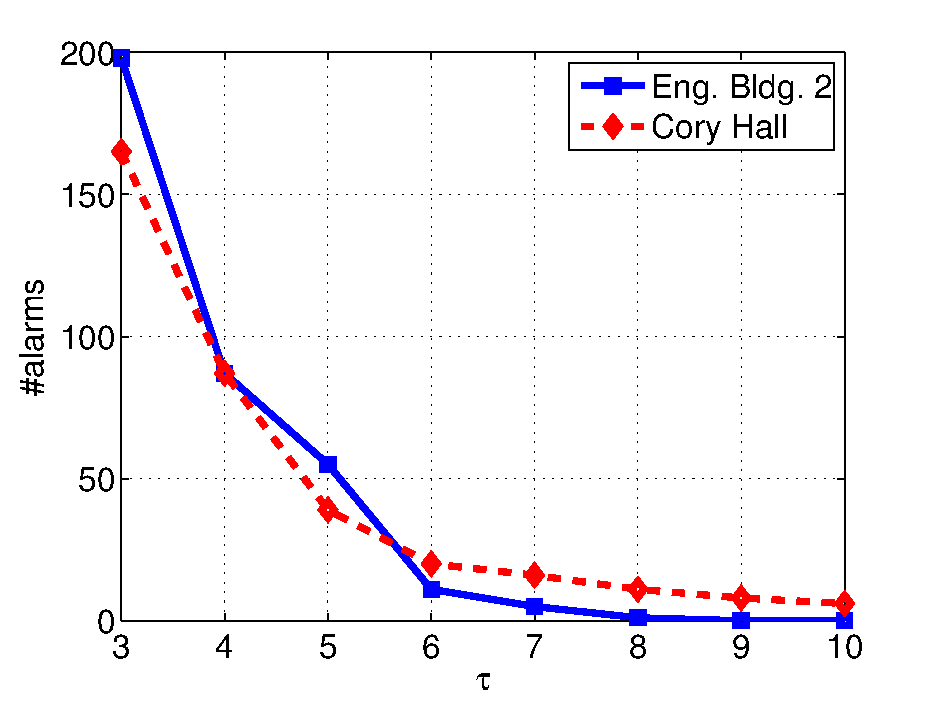
\includegraphics[width=.49\textwidth]{figs/threshold-eps-converted-to.pdf}
 \caption{Number of reported alarms for various threshold value ($\tau=[3,10]$).}
 \label{fig:thres}
 \end{center}
\end{figure}

\begin{table}
\begin{center}
\begin{tabular}{|l||c|c|c|c|c|}
\hline
&High&Low&Punc.&Missing&Other\\ \hline \hline
Eng. Bldg 2 & 9 (5) & 6 (5) & 1 (1) & 36 (1) & 3 (3) \\ \hline
Cory Hall & 25 (7) & 7 (3) & 4 (4) & 0 (0) & 3 (3) \\ \hline
\end{tabular}
\end{center}
\caption{Classification of the alarms reported by SBS for both dataset (and the number of corresponding anomalies).}
\label{tab:classif}
\end{table}

\paragraph{Experimental setup}
For each experiment, the data is split in time bins of one day, starting from 09:00 a.m. -- which is approximately 
the office's opening time.
We avoid having bins start at midnight since numerous anomalies appear at night and they are better highlighted if they are 
not spanning two time bins.
Only the data at medium frequencies are analyzed, the other frequency bands are ignored, and the reference matrix is computed from all time bins.


The threshold $\tau$ tunes the sensitivity of SBS, hence, the number of reported alarms.  
Furthermore, by plotting the number of alarms against the value of $\tau$ for both datasets (Figure \ref{fig:thres}) we observe an 
elbow in the graph around $\tau=5$.
With thresholds lower than this pivot value ($\tau<5$), the number of alarms significantly increases, causing less important anomalies 
to be reported.  
For higher values ($\tau>5$), the number of alarms is slowly decreasing, providing more conservative results that consist of the 
most important anomalies.
This pivot value provides a good trade off for either data set.

\begin{figure*}
  \subfloat[High power usage where the HVAC (EHP) is turned on at night\label{fig:res:eng1}]{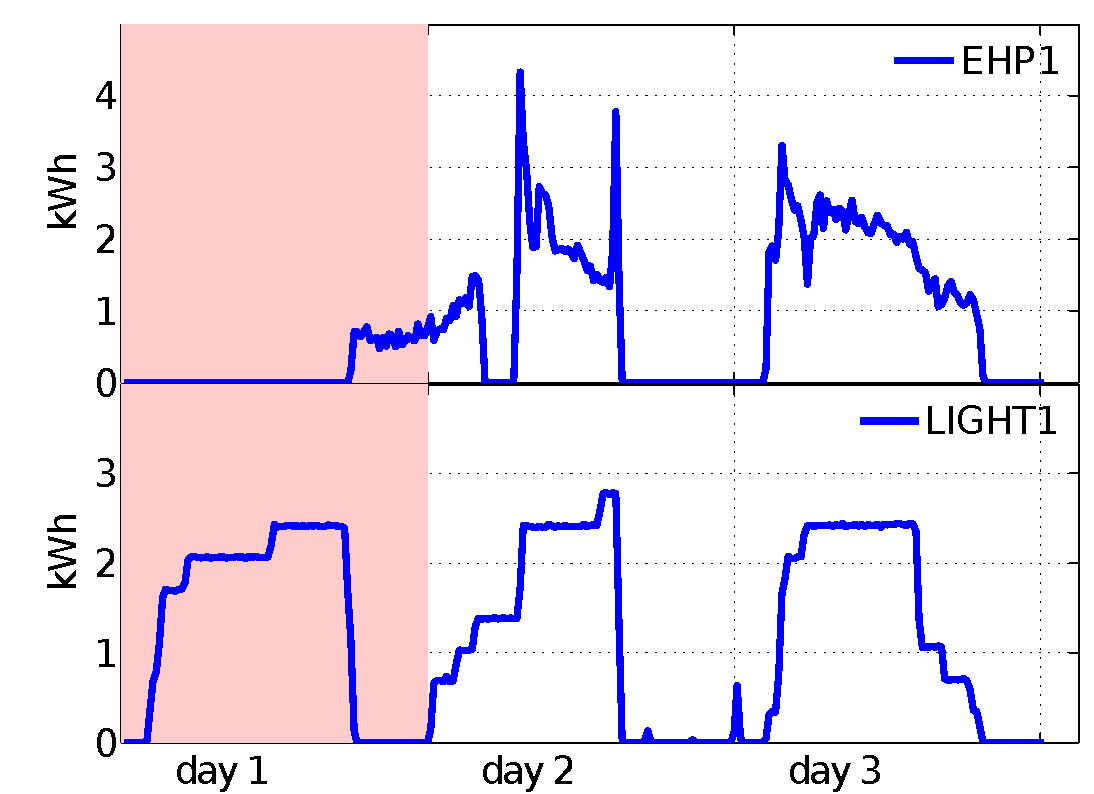
\includegraphics[width=.32\textwidth]{figs/0sig20_sig31alarm1-eps-converted-to.pdf}} \hspace{.015\textwidth} %EHP turned on at night!?
  \subfloat[High power usage where the light is left on at night\label{fig:res:eng2}]{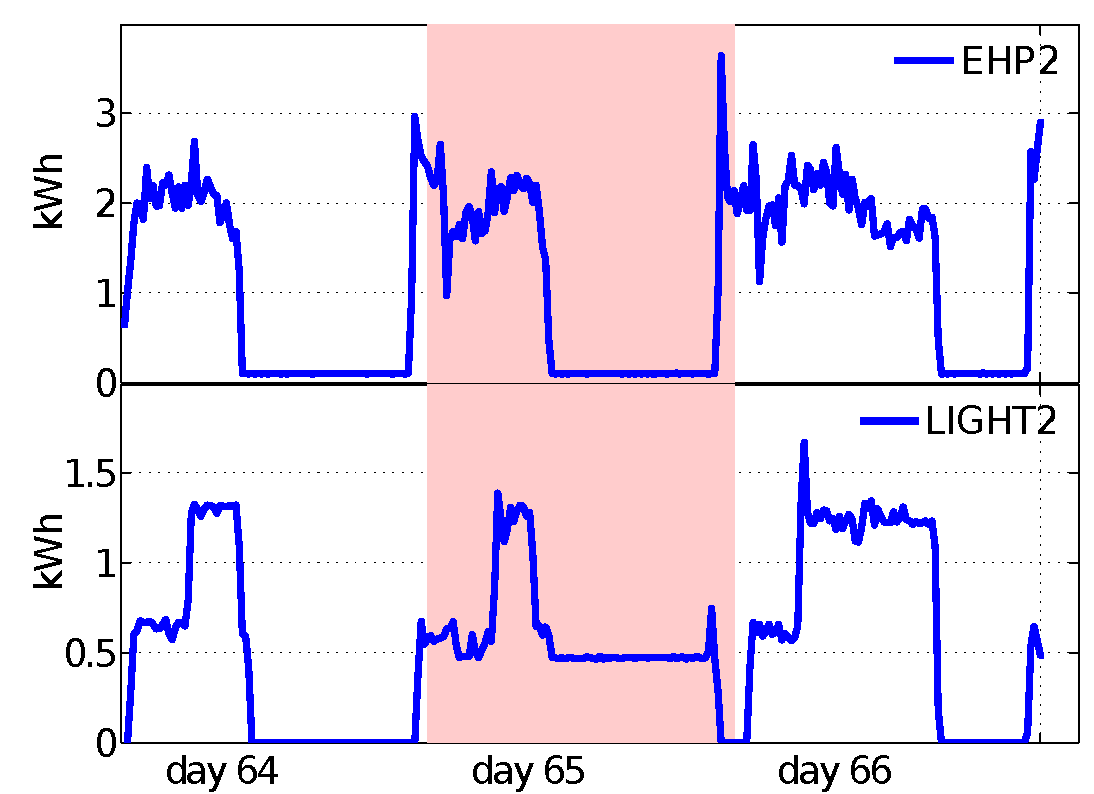
\includegraphics[width=.32\textwidth]{figs/0sig123_sig134alarm65-eps-converted-to.pdf}} \hspace{.015\textwidth}  %Light left on during night
 \subfloat[Low power usage where the HVAC (EHP) is not used during office hours\label{fig:res:eng3}]{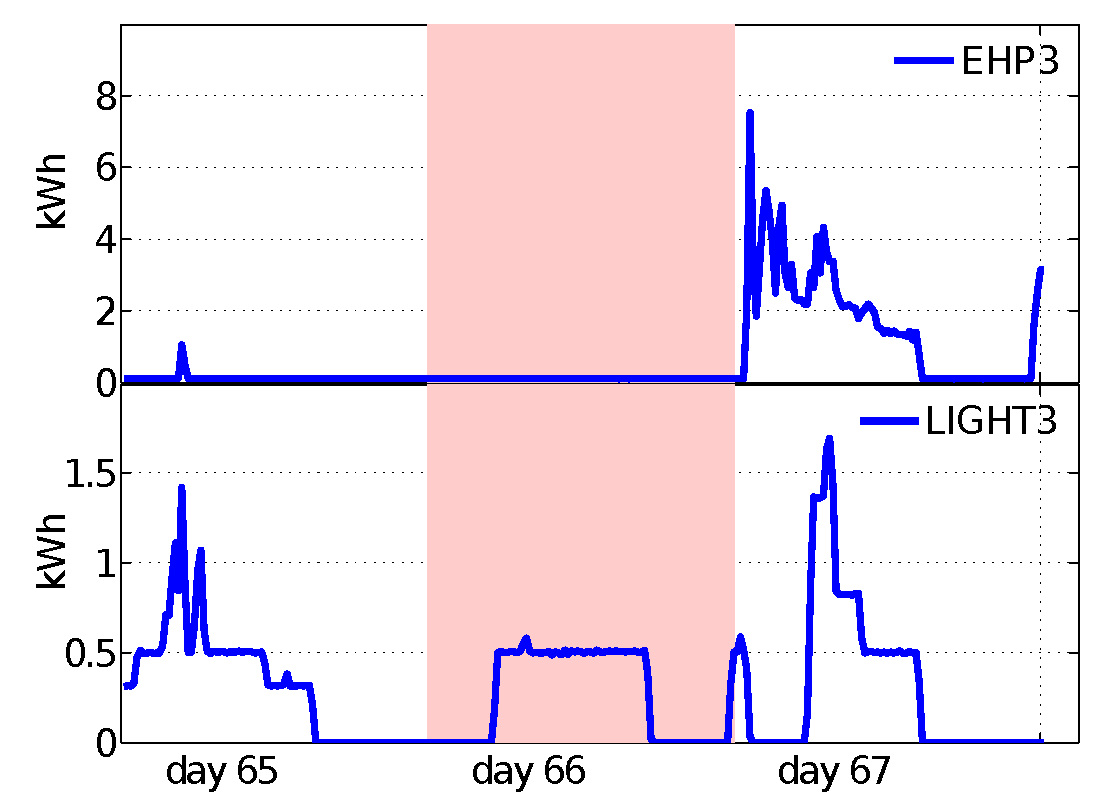
\includegraphics[width=.32\textwidth]{figs/0sig24_sig33alarm66-eps-converted-to.pdf}}\\ %Three EHPs that are really correlated
 \subfloat[Long term high power usage partially detected\label{fig:res:eng4}]{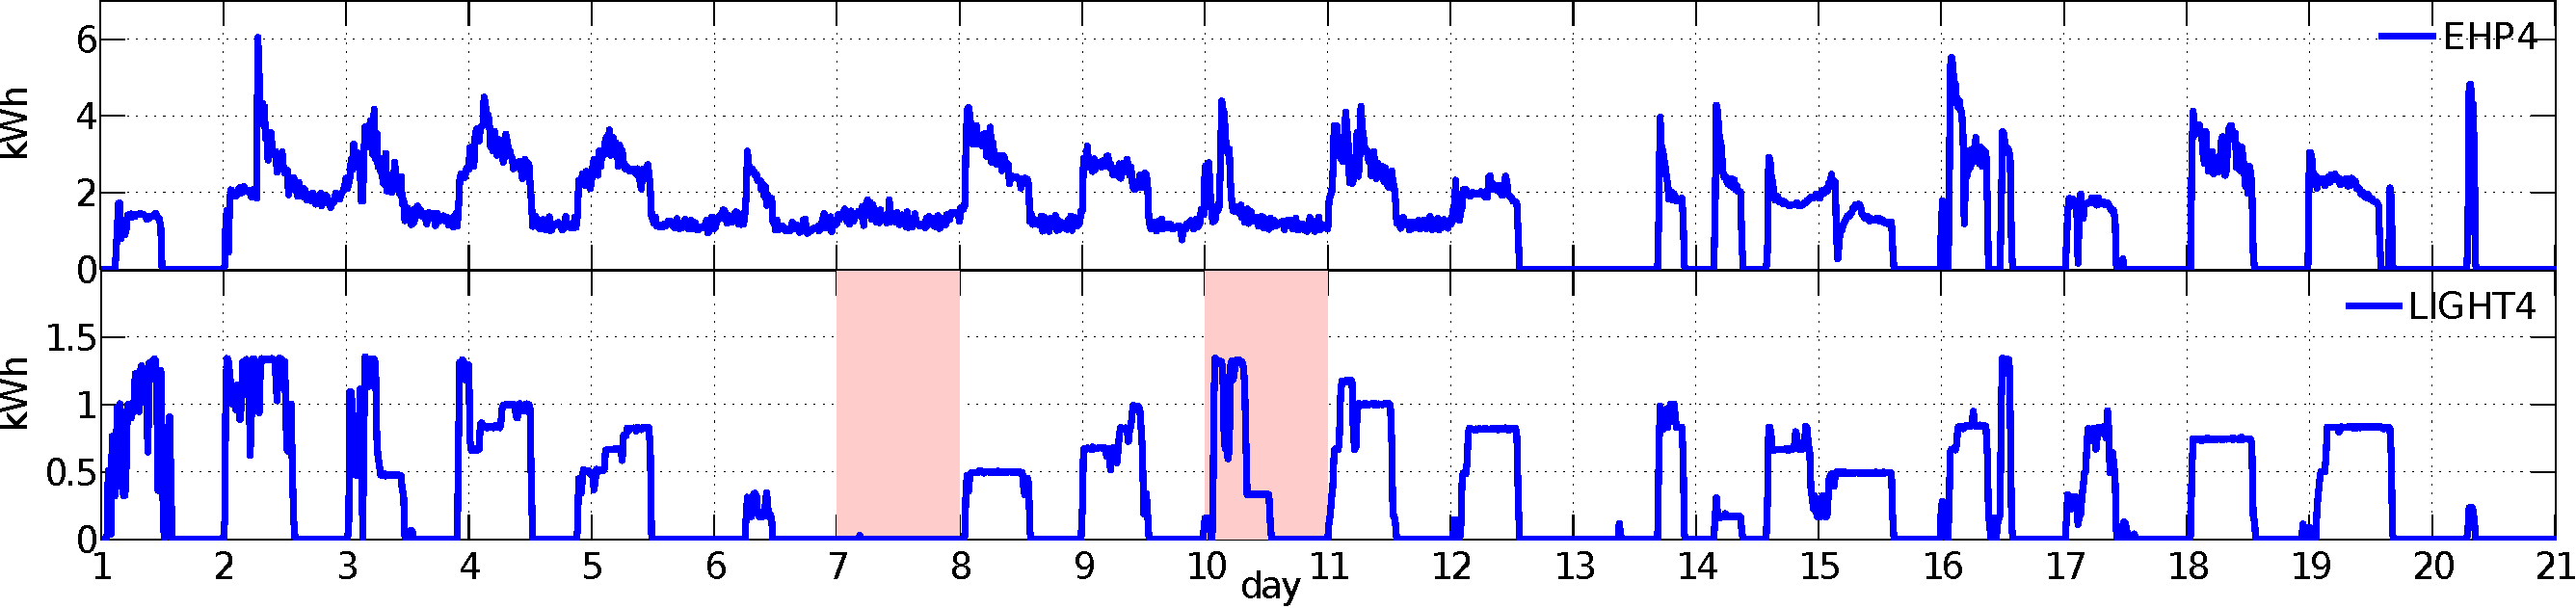
\includegraphics[width=\textwidth]{figs/0sig3_sig15alarm7-eps-converted-to.pdf}}\\  
\caption{Example of alarms (red rectangles) reported by SBS on the Eng. Bldg 2 dataset}
\end{figure*}


Table \ref{tab:classif} classifies the alarms reported by SBS on both datasets.
 Anomalies spanning several time bins (or involving several devices) may raise several alarms.  We display these in Table \ref{tab:classif} 
 as numbers in brackets -- the number of anomalies corresponding to the reported alarms.
%Due to page limitation the following sections only present the most typical and interesting anomalies identified by SBS.

\subsubsection{Engineering Building 2}


SBS reported 55 alarms over the 10 weeks of the Eng. Bldg 2 dataset.
However, 36 alarms are set aside because of sensor errors; one GHP has missing data for the first 18 days.
Since this device is highly correlated to the GHP in the reference matrix, their relationship is broken for the 18 first bins and 
for each bin one alarm per device is raised.

\begin{figure*}
  \subfloat[Low power usage due to a chiller failure\label{fig:res:cory1}]{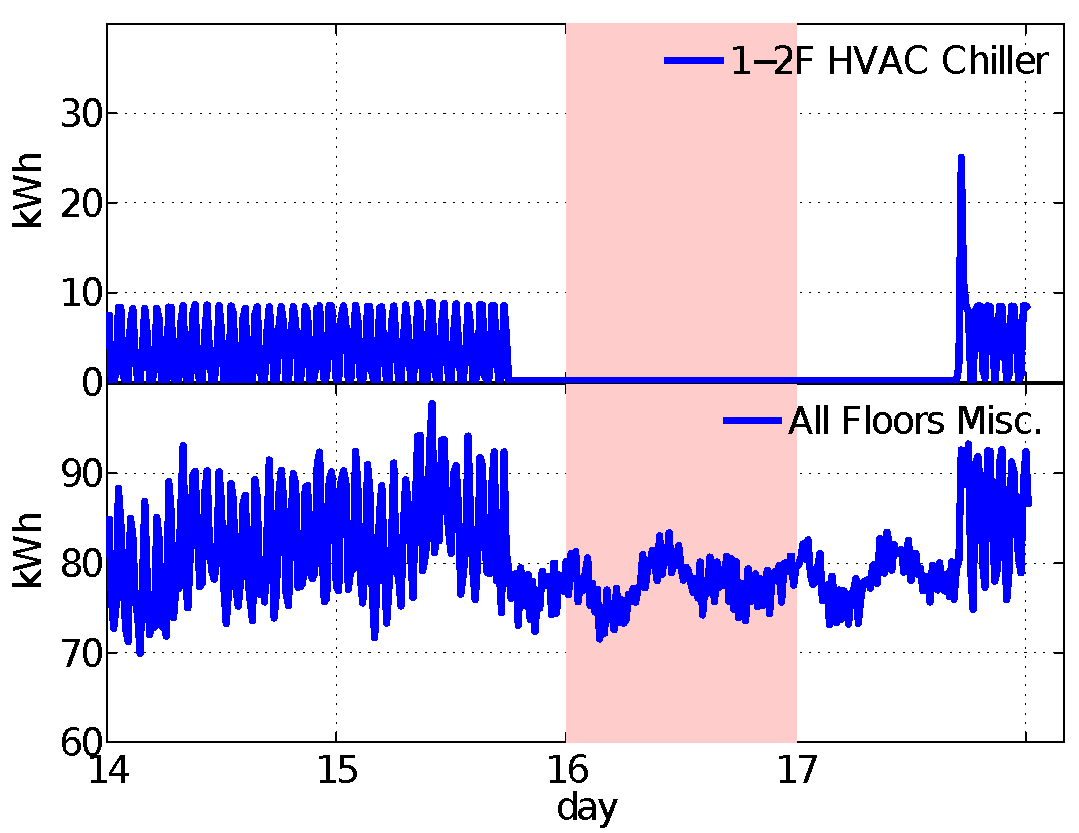
\includegraphics[width=.32\textwidth]{figs/1sig37_sig55alarm16-eps-converted-to.pdf}} \hspace{.015\textwidth}
 \subfloat[High power usage highlighted by the elevator usage\label{fig:res:cory21}]{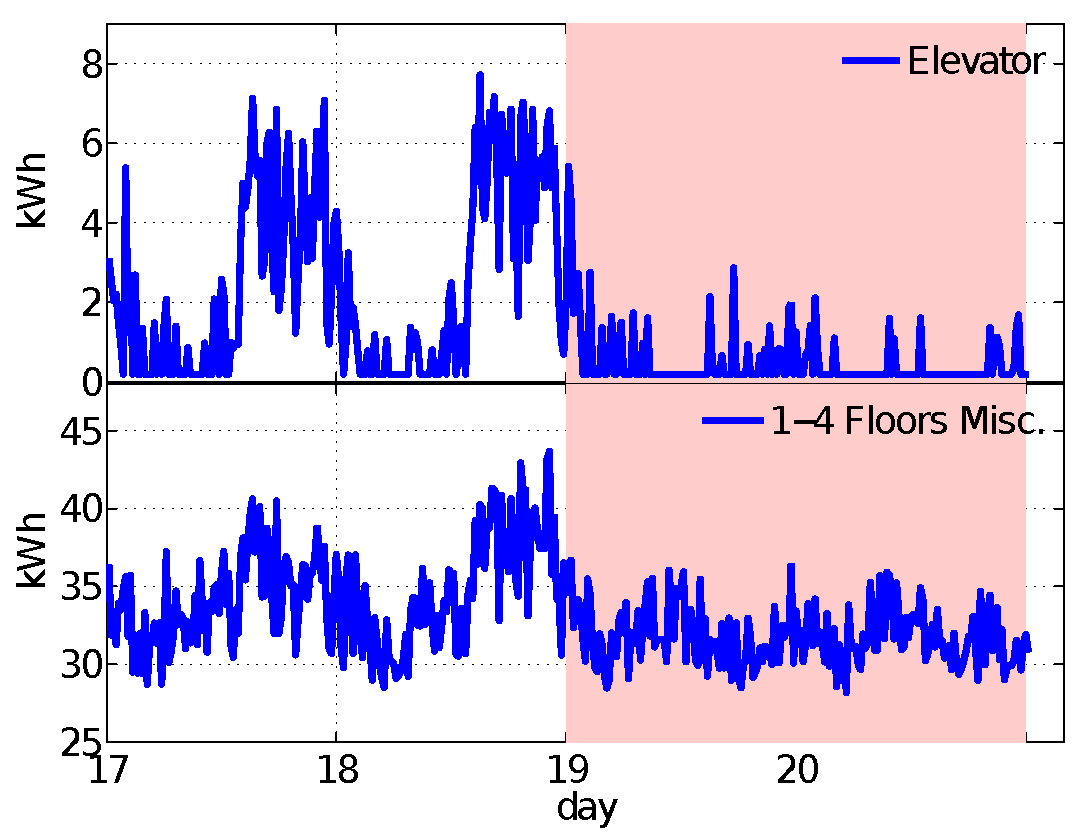
\includegraphics[width=.32\textwidth]{figs/1sig7_sig49alarm19-eps-converted-to.pdf}}
 \hspace{.015\textwidth}
 \subfloat[Normal power and elevator usage\label{fig:res:cory22}]{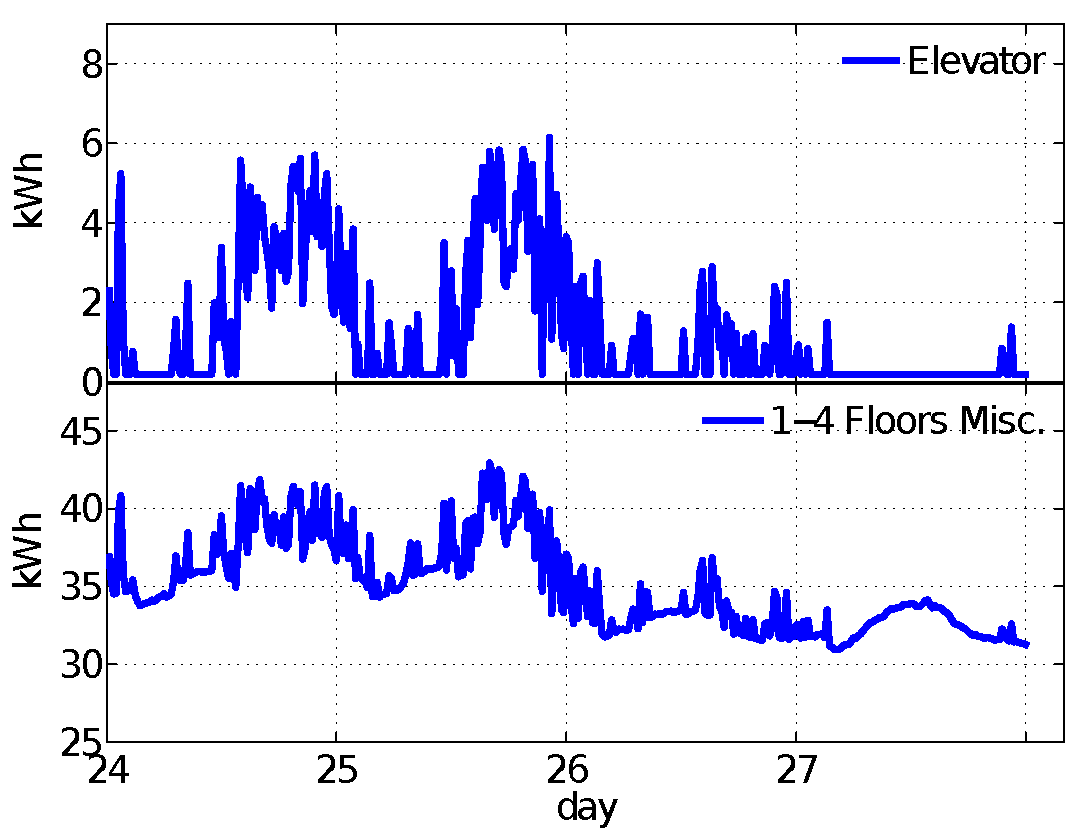
\includegraphics[width=.32\textwidth]{figs/1sig7_sig49alarm-eps-converted-to.pdf}}\\ 
 \subfloat[Long term high power usage due to competing heating and cooling\label{fig:res:cory3}]{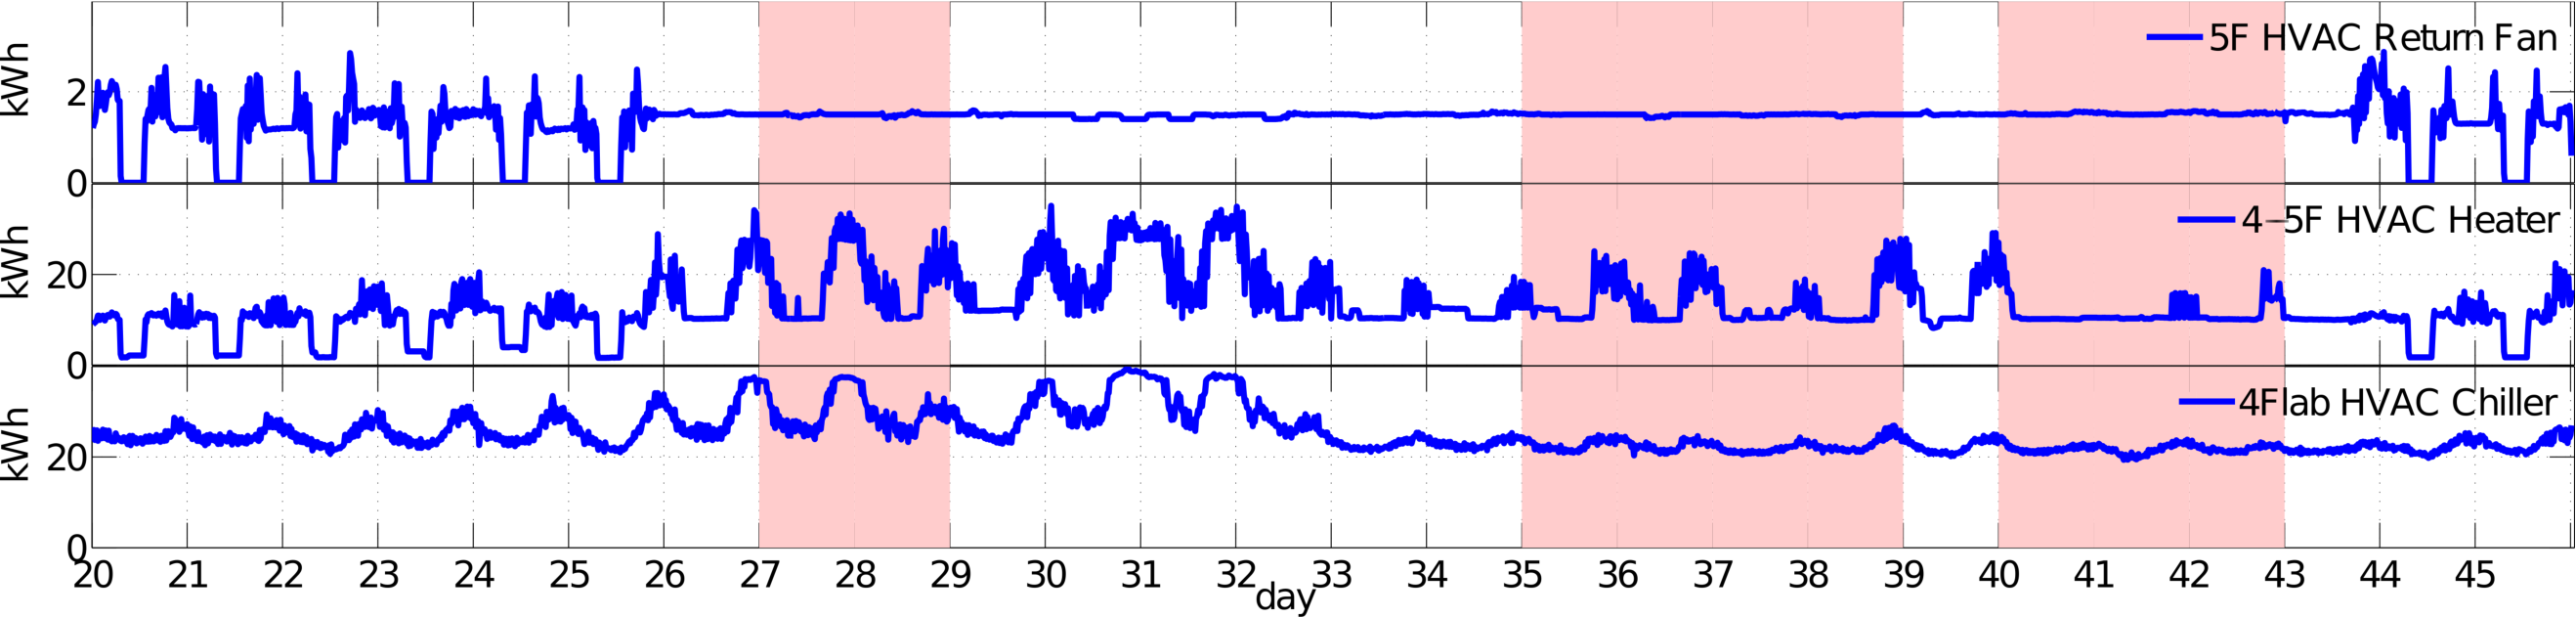
\includegraphics[width=\textwidth]{figs/1sig34_sig54alarm27-eps-converted-to.pdf}} 
\caption{Example of alarms (red rectangles) reported by SBS on the Cory Hall dataset}
\end{figure*}

In spite of the post-Fukushima measures to reduce Eng. Bldg 2's energy consumption, 
SBS reported 9 alarms corresponding to high power usage (Table \ref{tab:classif}).
Figure \ref{fig:res:eng1} depicts the electricity consumption of the light and EHP in the same room where two alarms are raised.
Because the EHP was not used during daytime (but is turned on at night, when the light is turned off) the relationship between the two devices 
is ``broken'' and an alarm is raised for each device.
Figure \ref{fig:res:eng2} shows another example of energy waste.  The light is on at night and the EHP is off.
The top-priority anomaly reported by SBS is caused by the 10 days long constant use of an EHP (Figure \ref{fig:res:eng4}) and this 
waste of electricity accounts for 165 kWh.
SBS partially reports this anomaly but lower values of $\tau$ permits us to identify most of it.


We observed 6 alarms corresponding to abnormally low power use.  Upon further inspection we notice that it corresponds to energy saving
 initiatives from the occupants -- likely due to electricity concerns in Japan.
This behavior is displayed in Figure \ref{fig:res:eng3}.  The room is occupied at the usual office hours (indicated by light usage)  but the 
EHP is not on in order to save electricity.

\subsubsection{Cory Hall}
SBS reported 39 alarms for the Cory Hall dataset (Table \ref{tab:classif}).
 7 are classified as low power usage, however, our inspection revealed that the root causes are different than for the Eng. Bldg 2 dataset.
We observe that the low power usage usually corresponds to device failures or misconfiguration.  
For example, Figure \ref{fig:res:cory1} depicts the electricity consumption of the $2^{nd}$ floor chiller and a power riser that comprises the consumption of multiple systems, including the chiller.
As the chiller suddenly stops working, the correlation between both measurements is significantly altered and an alarm for each device is raised.

SBS also reports 25 alarms corresponding to high power usage. 
One of the identified anomalies is particularly interesting.
We indirectly observe abnormal usage of a device from the power consumption of the elevator and a power panel for equipment from 
the $1^{st}$ to the $4^{th}$ floor.
Figure~\ref{fig:res:cory21} and~\ref{fig:res:cory22} show the electricity consumption for both devices. 
SBS uncovers the correlation between the these two signals, as the amount of electricity going through the panel fluctuates along with the elevator power consumption (Figure \ref{fig:res:cory22}).
In fact, the elevator is a good indicator of the building's occupancy.
Anomalous energy-consumption is identified during a weekend as the consumption measured at the panel is independently fluctuating from the elevator usage.
These fluctuations are caused by a device that is not directly monitored.  Therefore, we could not identify the root cause more precisely. 
 Nevertheless, the alarm is worthwhile for building operators to start investigating.

The most important anomaly identified in Cory Hall is shown in Figure \ref{fig:res:cory3}.
This anomaly corresponds to the malfunctioning of the HVAC heater serving the $4^{th}$ and $5^{th}$ floors. 
The heater is constantly working for 18 consecutive days, regardless of the underlying occupant activity.
Moreover, in order to maintain appropriate temperature this also results in an increase of the $4^{th}$ floor HVAC chiller power consumption 
and several fans, such as the one depicted in Figure \ref{fig:res:cory3}.
This situation is indicative of simultaneous heating and cooling -- whereby heating and cooling systems are competing -- and it 
is a well-know problem in building management that leads to significant energy waste.
For this example, the electricity waste is estimated around 2500 kWh for the heater.
Nevertheless, as the anomaly spans over 18 days, it is hidden in the building's overall consumption, thus, it is difficult to detect 
by building administrators without SBS.












\section{Spatial Verification and Empirical Mode Decomposition}

\section{Dataset}
The data we used was obtained from a deployment of sensors in a 12-story office building
on the campus of the University of Tokyo~\cite{gutp, ogawa:lncs2011}.  The deployment consists of 
almost 700 sensors monitoring device power consumption, ranging from plug-load devices to components of the
heating, ventilation, and air conditioning system (HVAC) and lighting.  Sensors also reported temperature, 
pressure, device-state, and other information.  Each sensor reports data on the
order of minutes.  Over 500 GBs of data was collected over a 2-year span.

\begin{figure*}[tb]
\hspace{-2cm}
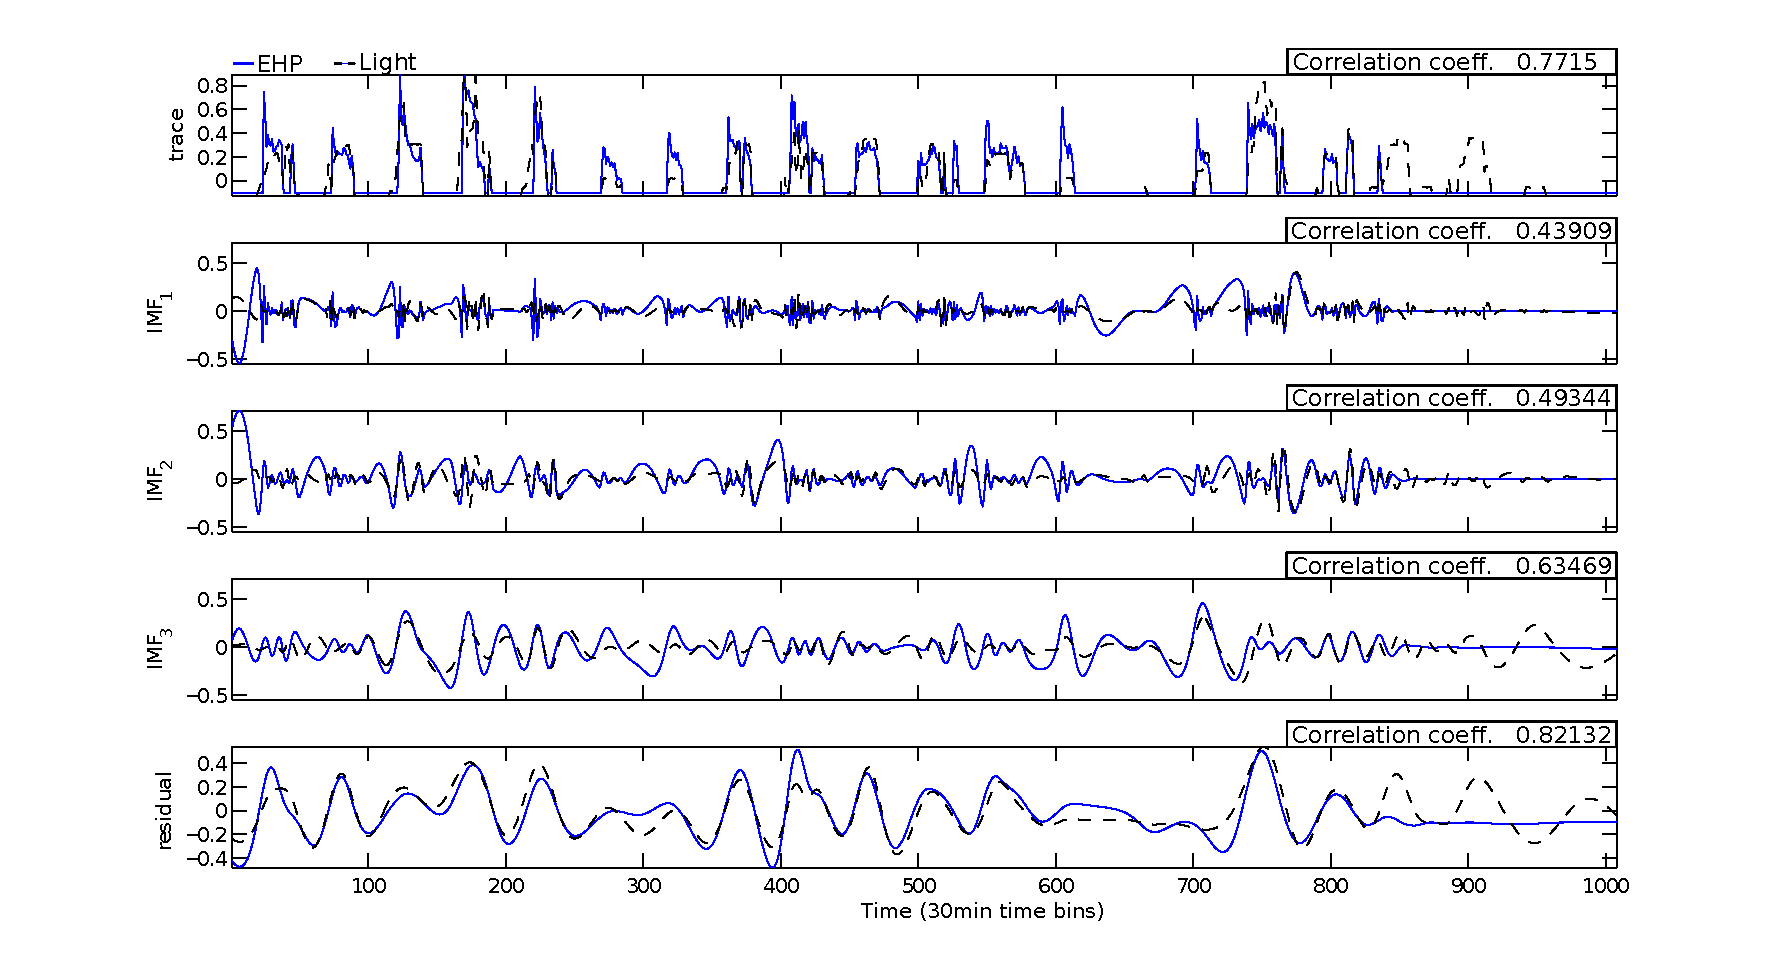
\includegraphics[width=1.2\textwidth]{img/emd_25_26-eps-converted-to}
\vspace{-1cm}
\caption{Decomposition of the EHP and light trace using bivariate EMD. IMFs correlation coefficients highlight the intrinsic relationship of the two traces.}
\label{fig:emd}
\end{figure*}

% The intent of the Green University of Tokyo Project (GUTP) \cite{gutp} is to reduce the university environmental impacts associated to its electric energy consumption.
% The first step of this project was to deploy sensors at the Building No.2 of the Faculty of Engineering 
% Electric power consumption of a 12 floors building containing researchers office and classroom.
% 1215 sensors monitoring different devices...

%received attention in the past \cite{ogawa:lncs2011}.

For this investigation, we focus on a three-week span in the summer of 2011 (from July 4th to July 24th).
The dataset captures regular work days, weekends, and one holiday (July 18th).  This timeframe captures
the typical usage of the equipment, triggered by occupant activity.  For the initial
analysis, we focus on three sensors; two water pumps and a light feed.  The first pump is an 
``electric heat pump'' and is labled as EHP, the second  is a ``gas heat pump''
and labeled as GHP.  The room lighting system serves the same room as the EHP.  The GHP
serve a different room on the same floor.  The expanded portion of our analysis pivots as the EHP
and does a pairwise comparison between it and all other sensors in the building.

% includes one day holiday (July 18th)
% 3 different sensors:
% \begin{itemize}
%  \item Two are measuring the electric power consumption of two devices from the same room; an electric heat 
%  		pump (EHP) and the room lighting system.
%  \item One is measuring the electric power consumption of a gas heat pump (GHP) that is pumping water to cool 
%  		a different room in the same building.
% \end{itemize}

% Later we expand our analysis to include all the sensors in the building.


\section{Problem statement and Initial approach}\label{problem}
% In our analysis, we are focused on finding devices that are correlated in their use over time.  Therefore, the
% main objective is to examine how device traces relate to one another.  The wish to identify
% correlated device-trace patterns at large spatio-temporal scales.

In buildings, metadata is poorly and unsystematically managed within a single system domain.  Moreover, 
with the ever growing number of additional sub-meters, it is important to quickly integrate
sensor data from multiple systems to understand the full state of the building.  It is also important to 
understand how sensors are used in concert.  Anamolies in usage may indicate underlying problems with 
the equipment or inefficient/incorrect usage.  

We begin our analysis by running direct correlation between the traces.
Figure \ref{fig:raw} shows the raw traces for the three devices discussed in 
the previous section (EHP, GHP, light).  All three exhibit a diurnal usage pattern.  On weekends, each
draw less power.  The correlation coefficient for 
 the EHP and light is $0.7715$ and the correlation coefficient for the EHP and GHP is $0.6370$.
Running correlation across them yields high correlation coefficients, mostly
due to their underlying daily usage pattern.

% Usual measures on sensor data like correlation coefficient or granger causality \cite{kim:buildsys2010}
% -- this is not working

\begin{figure}[t!]
\centering
 \subfigure[EHP trace]{\label{fig:raw_ehp}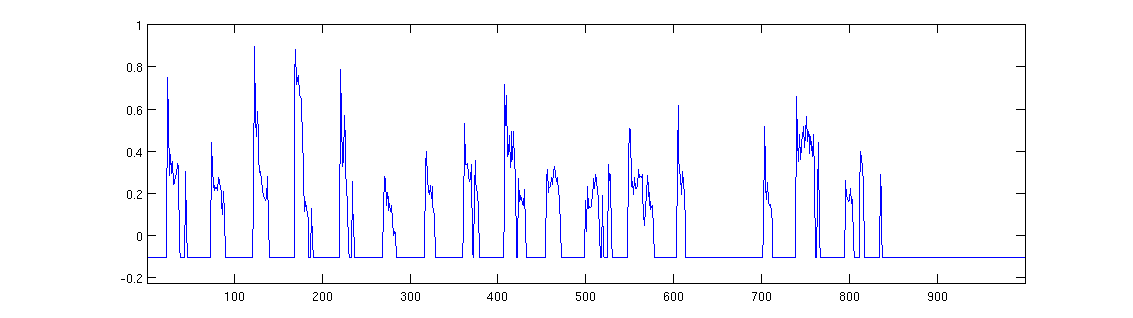
\includegraphics[width=.4\textwidth]{img/25.png}}
 \subfigure[Light trace]{\label{fig:raw_light}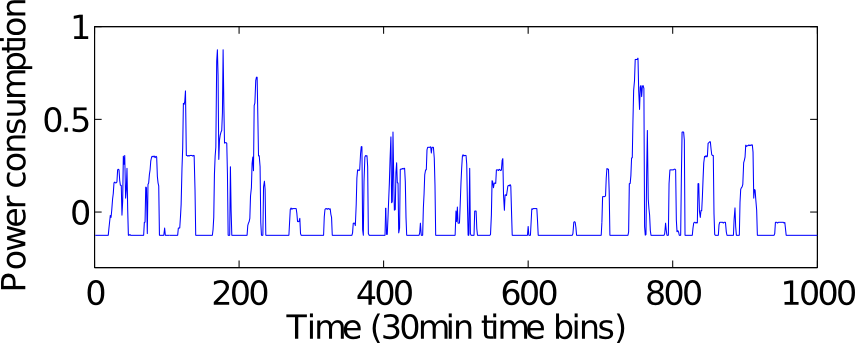
\includegraphics[width=.4\textwidth]{img/26.png}}
 \subfigure[GHP trace]{\label{fig:raw_ghp}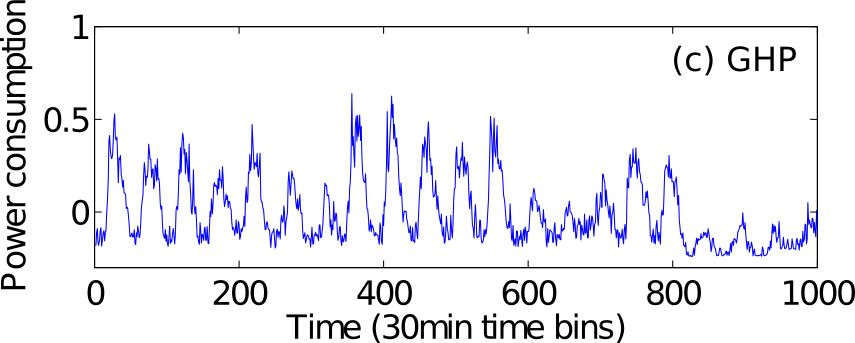
\includegraphics[width=.4\textwidth]{img/41.png}}
 \caption{Traces from three different sensors captured in 2011 from July 4th to July 24th. Data is normalized and aggregated into 30 minutes time bins.}
 \label{fig:raw}
\end{figure}

% For example correlation coefficients for the 3 signals...
% correlation coefficient for the EHP and Light signals: $0.772013$
% correlation coefficient for the EHP and GHP signals: $0.636967$

% These scores suggest that the EHP signal is related to the two other measured signals.

% These results were expected for the EHP and light traces, as the two measured devices operate for the same room 
% and are used simultaneously.  More importantly, they are used to support the occupants of the rooms they are serving.
% We were somewhat surprised by the magnitude of correlation between the pumps, since they serve rooms on
% opposite sides of the building and operate independently.  However, occupancy and weather patterns are similar,
% and the underlying trend is captured by the correlation calculation.
% The difference between the correlation coefficients is small and one might conclude that all three are
% closely related to one another.  That conclusion is not false but misleading.  Correlation on the raw 
% traces is sensitive to the underlying trend shared by the traces.  In order to meaningfully distinguish between
% truly related devices we need to remove the common trends. 

Our initial results were not surprising.  The diurnal pattern dominates the comparison between the sensors.
Weather is the main driver for this behavior and it affects the readings in almost all of the
sensors in our dataset.  Cross-correlation on raw sensor data is insufficient for filtering intrinsically related
behavior.  Upon closer examination of the data we assess the following:

\begin{itemize}
\item The main underlying diurnal trend occurs in almost all the traces.
\item Occupancy and room activities occur at random times during the day and change 
		at a higher frequency than weather patterns.
\item Sensors that serve the same location observe the same activities.  Therefore, their underlying
		measurements should be correlated.
\end{itemize}

In order to uncover these relationships we must remove low-frequency trends in the traces and
compare the readings at high frequencies.

% \begin{table}
% \begin{center}
% \begin{tabular}{|l|l|l|l|l|l|}
% \hline
% × & Raw trace & 1st IMF & 2nd IMF & 3rd IMF & Residual\\ \hline
% EHP, Light & 0.7715 & 0.43909 & 0.49344 & 0.63469 & 0.82132 \\ \hline
% EHP, GHP & 0.6370 & 0.0060274 & 0.063546 & 0.16764 & 0.79378 \\ \hline
% \end{tabular}
% \caption{Correlation coefficients of the analyzed trace and their IMFs uncovered by EMD}
% \label{tab:corr}
% \end{center}
% \end{table}
% \subsection{Simple Scenario}

\begin{figure*}[tb]
\hspace{-2cm}
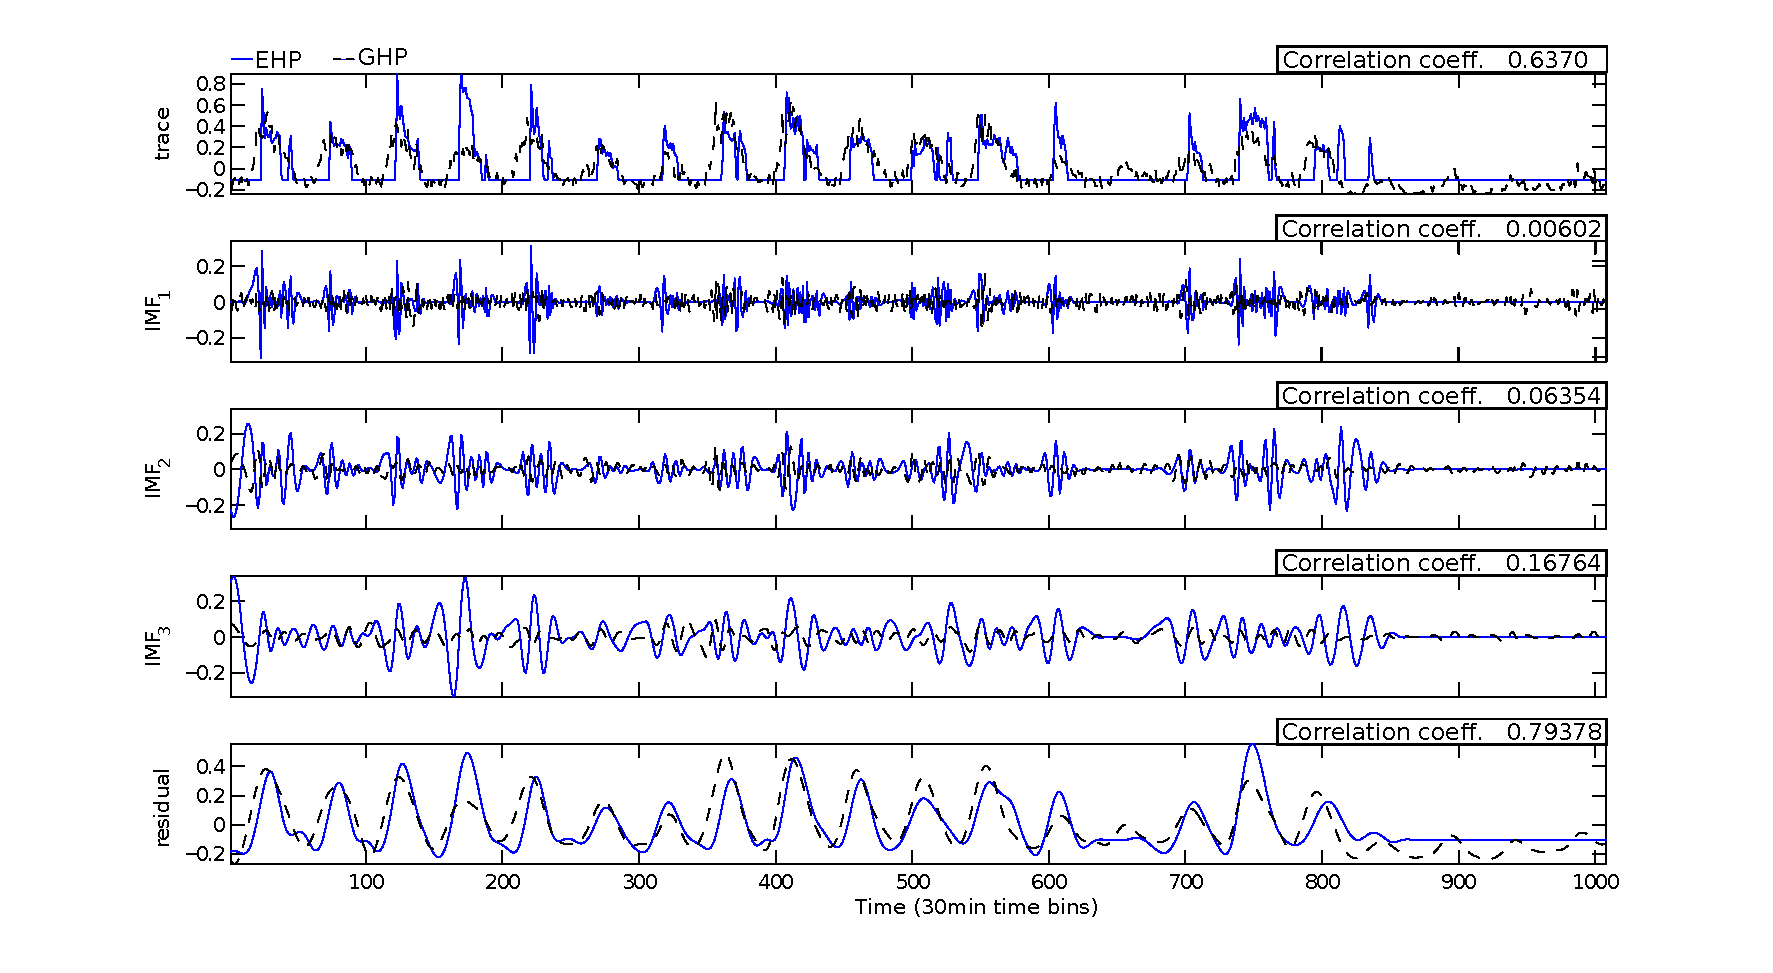
\includegraphics[width=1.2\textwidth]{img/emd_25_41-eps-converted-to}
\vspace{-1cm}
\caption{Decomposition of the EHP and GHP trace using bivariate EMD. IMFs correlation coefficients highlight the intrinsic independence of the two traces.}
\label{fig:emd2}
\end{figure*}

% The small difference between the two computed correlation coefficients is misleading as one could conclude that the three signals are correlated and the corresponding devices are activated by a single action.

% The high correlation coefficients obtained for these three signals result .... weekly pattern....
% small difference = local fluctuation...

% this high score comes from the fact that the two devices are monitoring offices that are weekly used.

% Indeed the weekly pattern of the data trump the correlation coefficients....

% How to inspect only the local fluctuations...?
% we'd like to have an elegant solution (i.e. not specifying the interesting time scale)


\section{Methodology}\label{method}
%Remove the weekly trend of the data to analyze the detailed changes that convey the device behavior at small time scales.

% Our initial approach examined correlation analysis on raw sensor traces.  However, we quickly
% found that correlation is overly sensitive to fluctuations in the data.
Fundamentally, the readings are driven by the same underlying phenomena: 
weather and occupancy.  Weather influences \emph{all} the data similarly.  Occupancy, however, changes
throughout the building and should be used as a differentiating component in the signal
comparisons.  Sensors that share spatio-temporal elements should be correlated after the removal
of the underlying trend driven by the weather.  In order to find unique relationships we needed to remove 
this common trend.

\subsection{Empirical Mode Decomposition}
Empirical Mode Decomposition (EMD) \cite{huang:emd1998} is a new techniques used for de-trending data.
Specifically, EMD detrends non-stationary, non-linear timeseries data.  A trend is defined as 
an intrinsically determined monotonic function within a certain temporal span or a function in which there 
can be at most one extremum within that temporal span.  A non-stationary signal is a signal whose mean and
variance change over time.  EMD is a process, rather than a theoretical tool.

We describe the process as follow:  for a signal \emph{X(t)}, let $m_1$ be the mean of its upper and
lower envelopes as determined from a cubic-spline interpolation of local maxima and minima. The locality 
is determined by an arbitrary parameter.

\begin{enumerate}
\item The first component $h_1$ is computed: $h_1=X(t)-m_1$
\item In the second sifting process, $h_1$ is treated as the data, and $m_{11}$ is the mean of $h_1$'s upper and lower envelopes: $h_{11}=h_1-m_{11}$
\item The procedure is repeated $k$ times, until $h_{1k}$ is a function: $h_{1(k-1)}-m_{1k}=h_{1k}$
\item Then it is designated as $c_1=h_{1k}$, the first functional component from the data, which contains the shortest period component of the signal. We separate it from the rest of the data: $X(t)-c_1 = r_1$, and the procedure is
repeated on $r_j: r_1-c_2 = r_2,\dots,r_{n-1} - c_n = r_n$
\end{enumerate}

The result is a set of functions called intrinsic mode functions (IMF); the number of functions in 
the set depends on the original signal~\cite{emd_process}.  An IMF is any 
function with the same number of extrema and zero crossings, with its envelopes being symmetric with respect to zero.
We run our correlation analysis on the shared IMF outputs between a pairs of signals.  In order to ensure 
that the IMFs corresponding to two distinct signals are on the same time scale, we use 
bivariate EMD \cite{rilling:biemd2007} to decompose two signals at once. The main use of EMD is for removing dominant trends to conduct a meaningful spectral analysis of the data.


\subsection{Results}

We test our hypothesis in this section by using EMD to remove low-frequency trends in the data
and run correlation calculation at overlapping IMF timescales.  We discover that EMD allows us
to find and compare high-frequency instrinsic behavior that is spatially correlated across
sensors.  We begin with a small set of three sensors (EHP, GHP, light) and expand our scope
to include all the sensors in the dataset.



\subsubsection{Initial analysis}
Lets consider the simple example of Section \ref{problem} where we would like to know if the EHP trace is correlated with the two other traces.
Recall that the correlation coefficients of the raw feeds was $0.7715$ and $0.6370$, corresponding to the light 
and GHP, respectively.
As stated in previous section this result is correct but not so meaningful, since most of the traces
display the same diurnal pattern.
Figure \ref{fig:emd} and Figure \ref{fig:emd2} show the EMD decomposition of the three traces.
For each trace, EMD has retrieved three IMFs that highlight the higher frequencies of the traces.

Figure~\ref{fig:emd} shows the normalized raw trace (top) and EMD output IMFs and residual as well as the 
correlation coefficients calculated on the IMFs for the EHP and
light traces.  The correlation coefficients are $0.43909$, $0.49344$ and $0.63469$ corresponding to the IMF1, 
IMF2, and IMF3, respectively.  Notice the high correlation between the high-frequency IMFs.
We know that the light and EHP serve the same room, and their high-frequency IMF correlation corroborates
our prior knowledge.
Figure~\ref{fig:emd2} shows a complementary result, for the EHP and GHP comparison.
The correlation coefficients for the EHP and GHP IMFs suggest that the two may be independent.  In fact, they
\emph{are} indepdent; they serve completely different rooms in the building!

EMD allows us to remove low-frequency trends that add noise to the original analysis.
By comparing IMFs, we see both intrisically correlated and \emph{uncorrelated} behavior.  In the next
section we expand our analysis and show the effectiveness of our methodology. 
% Although promising, these results must be validated across the rest of the
% dataset to confirm their significance.  


\subsubsection{Validation}
To validate the effectiveness of our approach, we analyze the same three-week time span for \emph{all} 674 
sensors deployed in the building.
For each trace $S$ we compute two scores: (1) the correlation coefficient between $S$ and the EHP trace
and (2) the average value of the IMF correlation coefficients.

\begin{figure}[tbh!]
\centering
 \subfloat[Raw traces correlation coefficients]{\label{fig:histo1}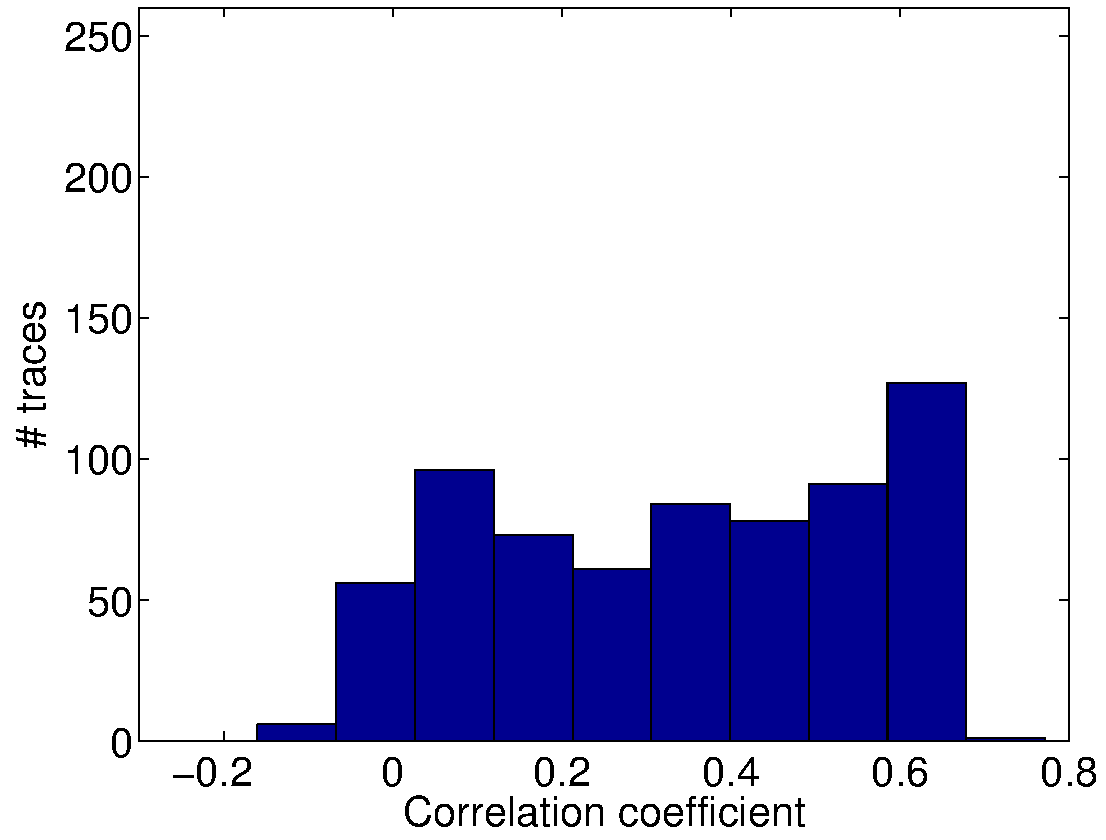
\includegraphics[width=.43\textwidth]{figs/allFloors_week1_week4_corr_abs-eps-converted-to}}
 \subfloat[Average IMFs correlation coefficients]{\label{fig:histo2}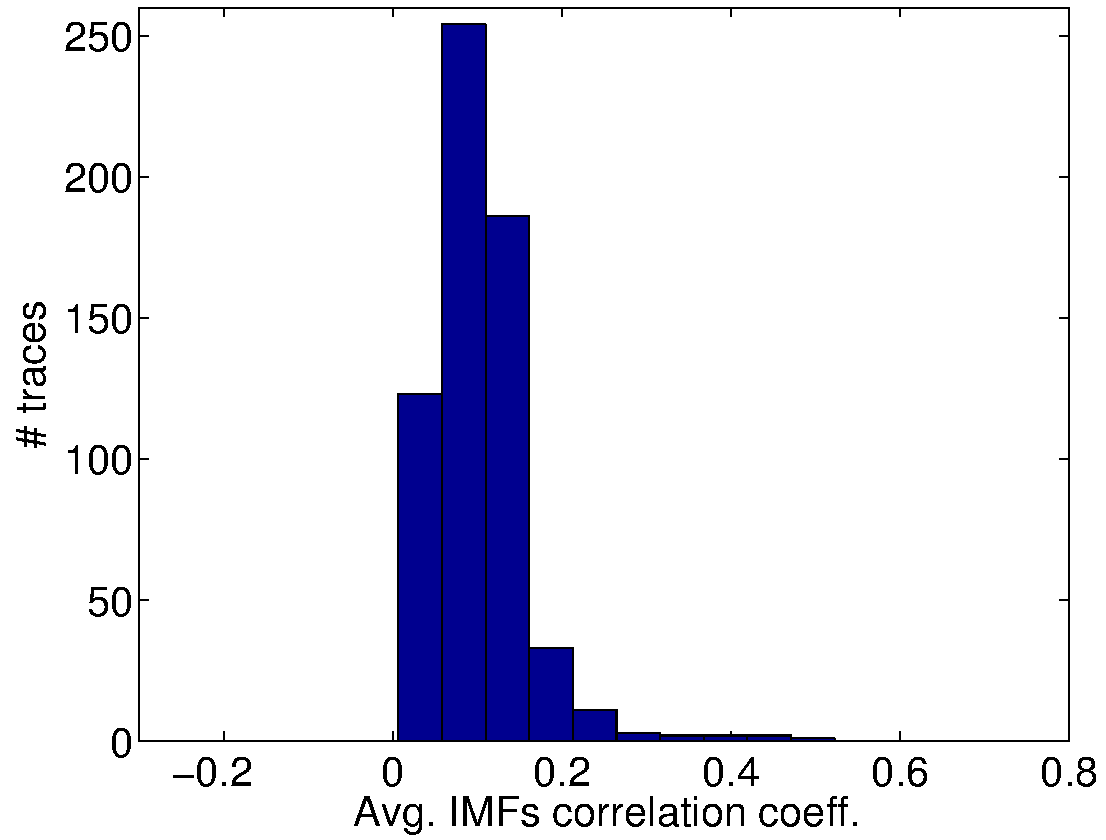
\includegraphics[width=.43\textwidth]{figs/allFloors_week1_week4_emd_abs-eps-converted-to}}
 \caption{Distribution of the correlation coefficients of the raw traces and correlation coefficients average of the corresponding IMFs using 3 weeks of data from 674 sensors.}
\label{fig:histo}
\end{figure}

\begin{figure}
\centering
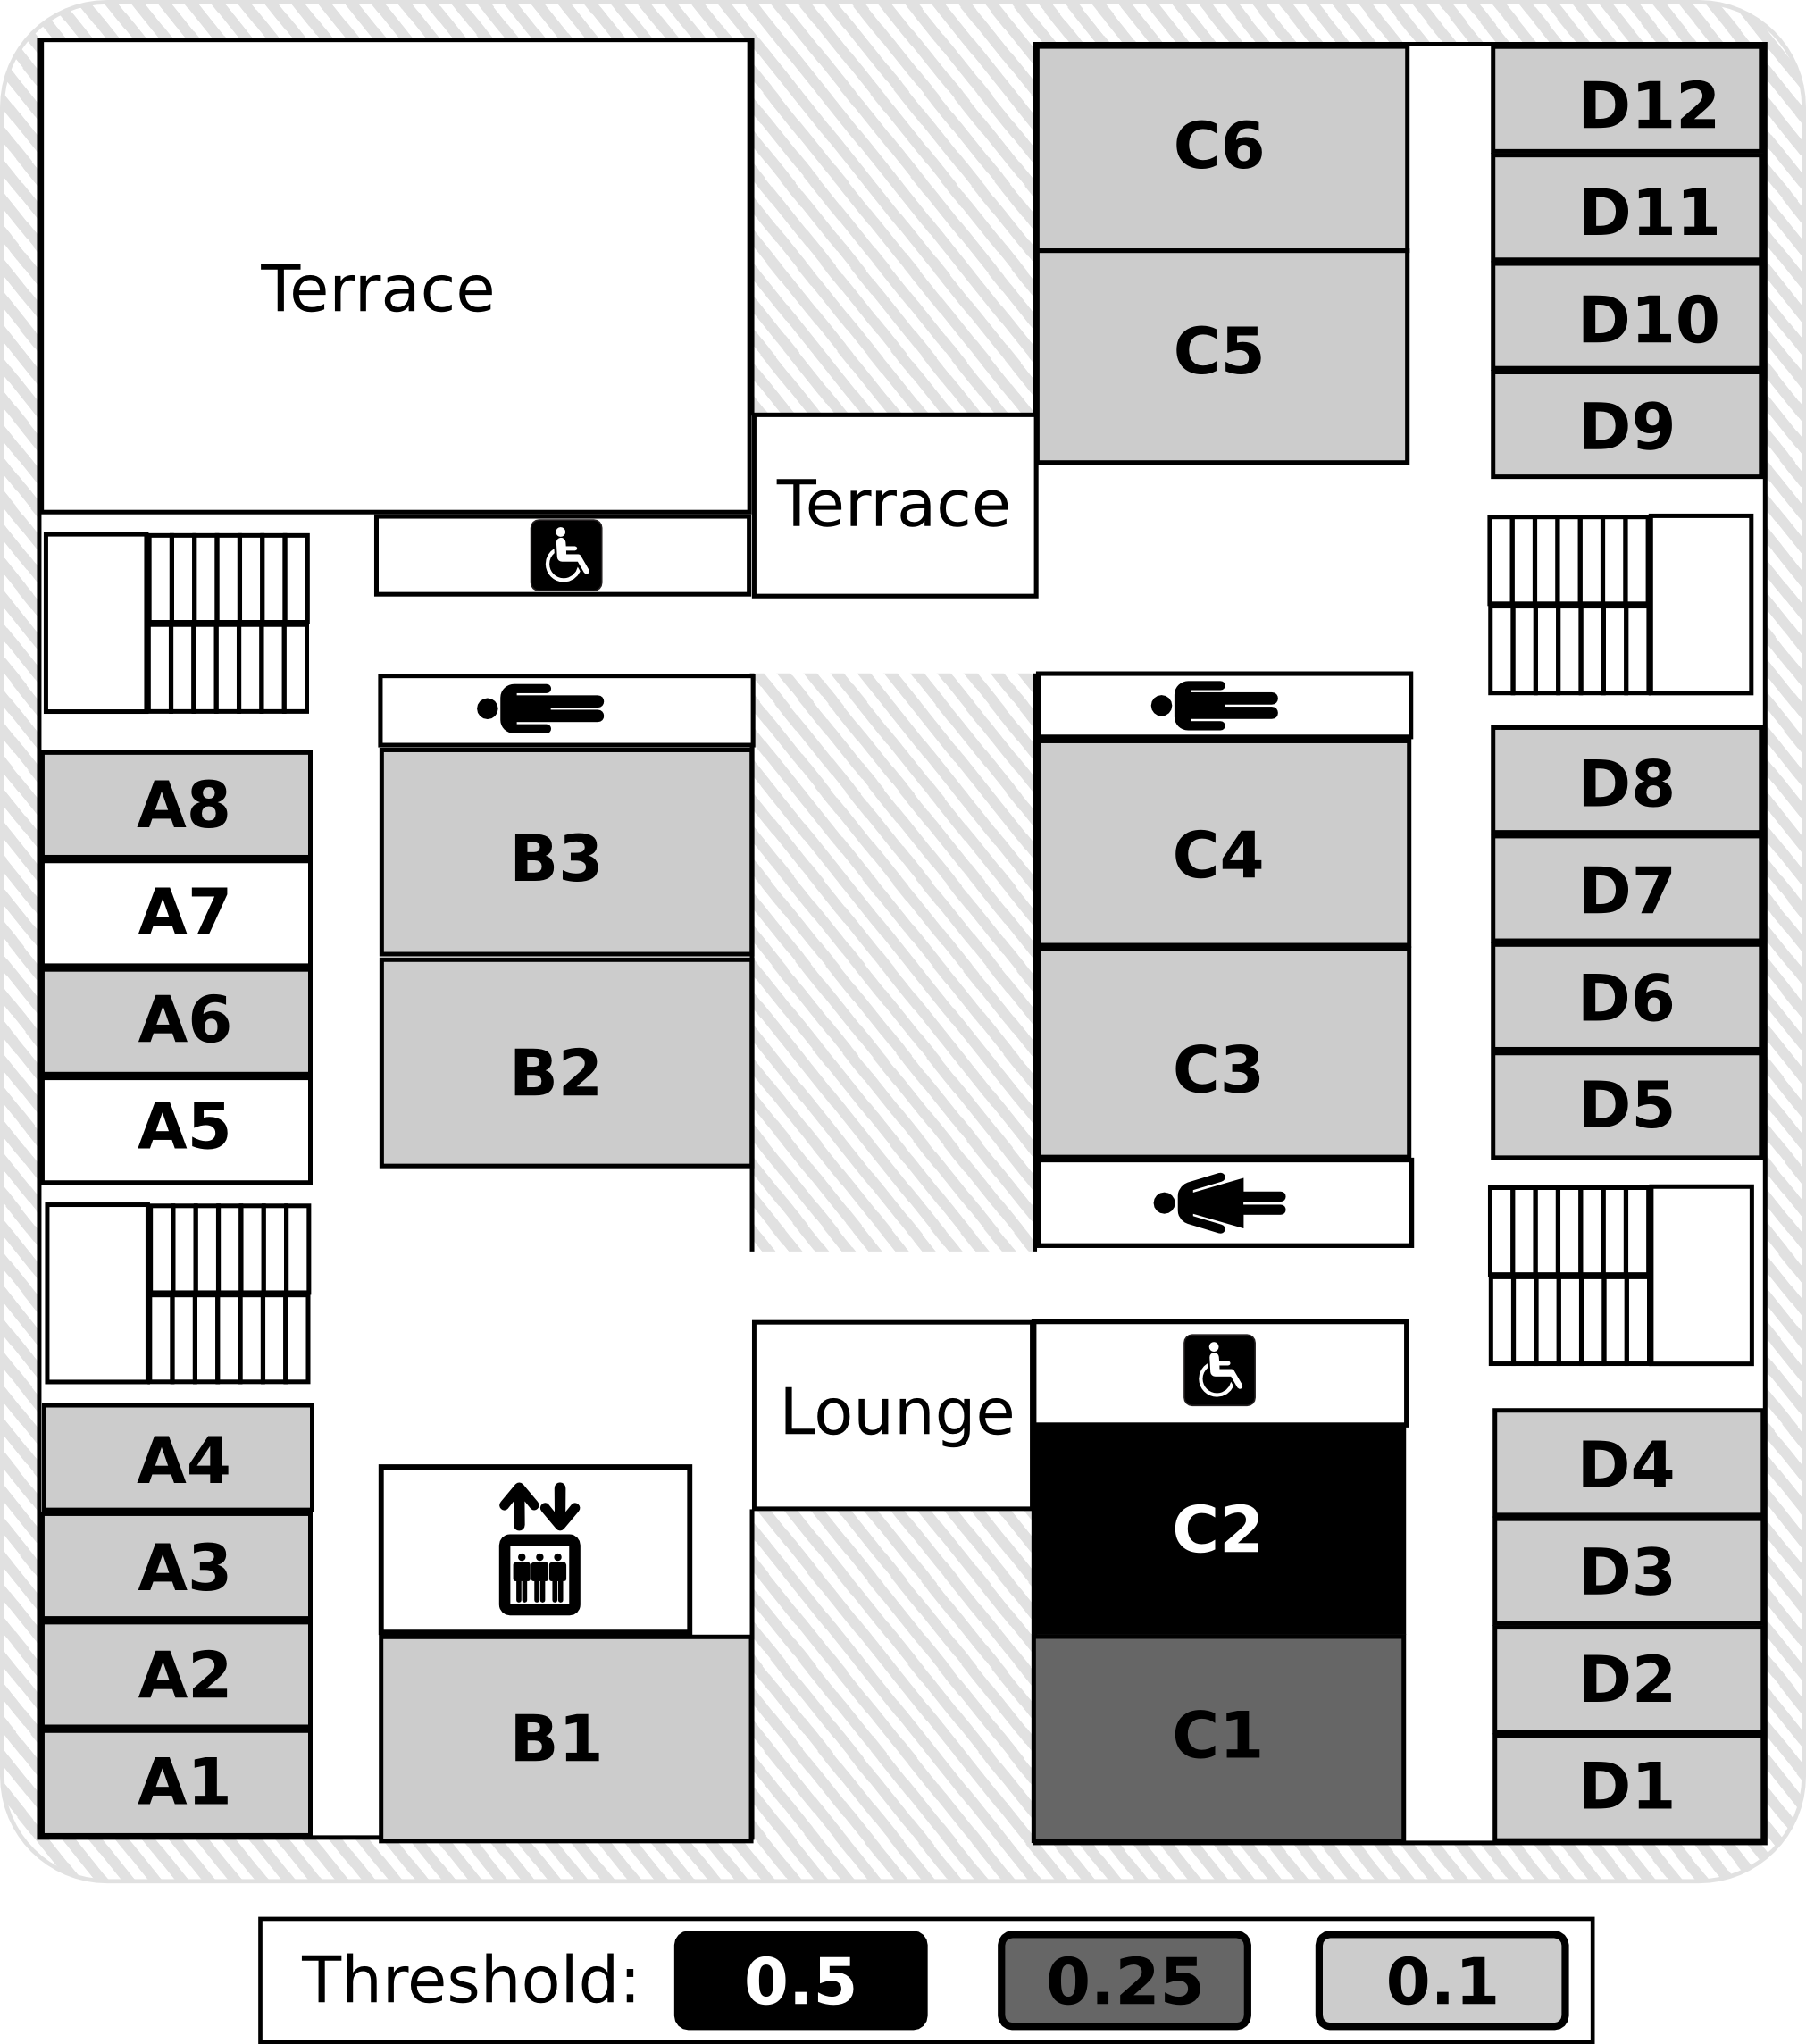
\includegraphics[width=.45\textwidth]{figs/floorMap.png}
\caption{Map of the floor where the analyzed EHP serves (room $C2$). The location of the sensors identified as related by the proposed approach are highlighted, showing a direct relationship between IMF correlation and spatial proximity.}
\label{fig:map}
\end{figure}

Figure \ref{fig:histo1} shows the distribution correlation coefficients.  Notice
that a large fraction of the dataset is correlated with the EHP trace.
\emph{Half} the traces have a correlation coefficient higher than $0.36$.  As expected, the underlying
trend is shared by a large number of device.
Although the highest score (i.e. $0.7715$) corresponds to the light in the same room that the EHP serves,
there are 118 pumps, serving all areas of the building, with a correlation higher than $0.6$.
Using only these results, it is not clear where the threshold should be set.  The distribution is close to 
uniform, making it difficult to 
know of how well your threshold discriminates against unrelated traces.
% Moreover, the distribution of the traces is almost uniform, thus, discriminating correlated traces is a laborious task.

Figure \ref{fig:histo2} shows the distribution of the average correlation value for the IMFs of
each trace and the EHP.  The number of traces correlated in the high frequency IMFs is significantly smaller
than the previous results. It's clear from the distribution that only a small set of devices are
\emph{intrinsically correlated} with the EHP.  In fact, \emph{only 10 traces out of 674} yielded a score higher than 
$0.25$. This allows us to easily rank traces by correlation.

Upon closer inspection of the 10 most correlated IMF traces, we find that there is a spatial relationship
between the EHP and the ten devices.  In fact, there is a direct relationship between score and distance from
the areas served by the EHP.  Figure~\ref{fig:map} shows a map of the floor that contains the rooms served by this
EHP.  The EHP directly serves room $C2$.  We introduce a correlation threshold to cluster correlated traces by score.
We highlight rooms by the threshold setting on the IMF correlation score.
When we set the threshold at $0.5$ we see that the sensors that have a correlation higher fall within room $C2$ --
the room served directly by the EHP.  As we relax the threshold, lowering it to $0.25$ and $0.1$ we see radial expansion from $C2$.  The trace with the highest score, $0.522$, is the trace corresponding to the lighting system \emph{in
the same room}.
The two highest scores for this floor (i.e. $0.316$ and $0.279$) are the light and EHP traces from next door, room $C1$.
Lower values correspond to sensors measuring activities in other rooms that have no specific relationship to the analyzed trace.  The results show a direct relationship between IMF correlation and spatial proximity and \emph{supports our initial
hypothesis}.


% Interestingly, the IMFs correlation coefficients reveal the spatial correlation of the sensors.
% Figure \ref{fig:map} is the map floor where the EHP trace is measured.
% Specifically, the EHP reports heating activity in the room $C2$.
% in the simple scenario the GHP is located in the room A5.




Typically, placement information is embedded in the name or associated metadata for each sensor in the building.
These are used to group sensors by location.  For example, in our building data, all sensors that contain the string
 `410' in their name are in room 410.  Processes typically group streams in this fashion: using regular-expression matching 
or field-matching queries on the characters in the sensor name or metadata.  If these are not updated to reflect changes
then such group-by query results will not accurately represent true spatial relationships.  
Fontugne et al.~\cite{IOT} observe that spatial associations can be derived empirically.  We start with this approach in our 
work and explore, more deeply, the extent to which it can be used 
as a verification tool for corroborating the groups constructed from character-matching queries.  We refer
to this process as \emph{spatial verification}.

Prior work~\cite{IOT} makes use of a technique called Empirical Mode Decomposition (EMD)~\cite{EMD} to statistically cluster correlated
usage patterns.  Sensors close to each other show strong statistical correlations while sensors further apart show weaker correlations.  
The main parameter in their approach, the correlation threshold, is explored to demonstrate how it relates to characteristic spatial patterns
 in the sensor feeds.  However, they do not characterize the threshold as it relates to physical configuration.
Fontugne et al.~\cite{SBS} expand the work by applying EMD to uncover functional device patterns.  They develop
an unsupervised learning method to model normal usage patterns and apply an anomaly detection algorithm to alert when patterns
have deviated from the norm.  The methodology used in their work divides raw signals into four separate frequency bands
and shows the medium band to carry the most spatial information.

In this section, we explore the threshold parameter in~\cite{IOT} more deeply, in order to move towards automatic spatial clustering, 
to be used as a form of verification. We use EMD and the intrinsic mode function (IMF) re-aggregation methodology described in~\cite{SBS}, with some modifications, to statistically analyze the threshold parameter
and its relationship to spatial separation in a building.  We explore the hypothesis that \emph{a statistical boundary, analogous to a physical one,
exists and is empirically discoverable}.
We conduct an empirical analysis on the data collected from 15 sensors in 5 rooms over a one-month period.  Our study makes the following contributions:

\begin{itemize}
\item We corroborate the results in~\cite{IOT}, verifying the spatial correlation pattern in a very different building.
\item We characterize the correlation coefficient (corrcoeff) distribution of sensors in the same room and different rooms and validate our existence hypothesis for this preliminary sample.
\item We demonstrate that the statistical boundary between sensors in various rooms converges to a similar value and this value generalizes across rooms in this study.
\item We show the tradeoff between the true and false positive rate inherent to threshold selection. We also show that our method improves the classification accuracy from 80\% to 93.3\%.
\end{itemize}

Our results are promising yet preliminary.  We are able to find a statistical separation across a small number of rooms, quite well.
Our study, however, does not explore the extent to which the physical separation affects the results.  Certainly for rooms that
are far apart we observe a statistical distinction using our methodology.  However, we also find that in some cases, our approach
does not work as well.  We discuss the approach and results in the rest of the paper, followed by a short discussion and future work.

\begin{figure*}[ht!]
\centering
    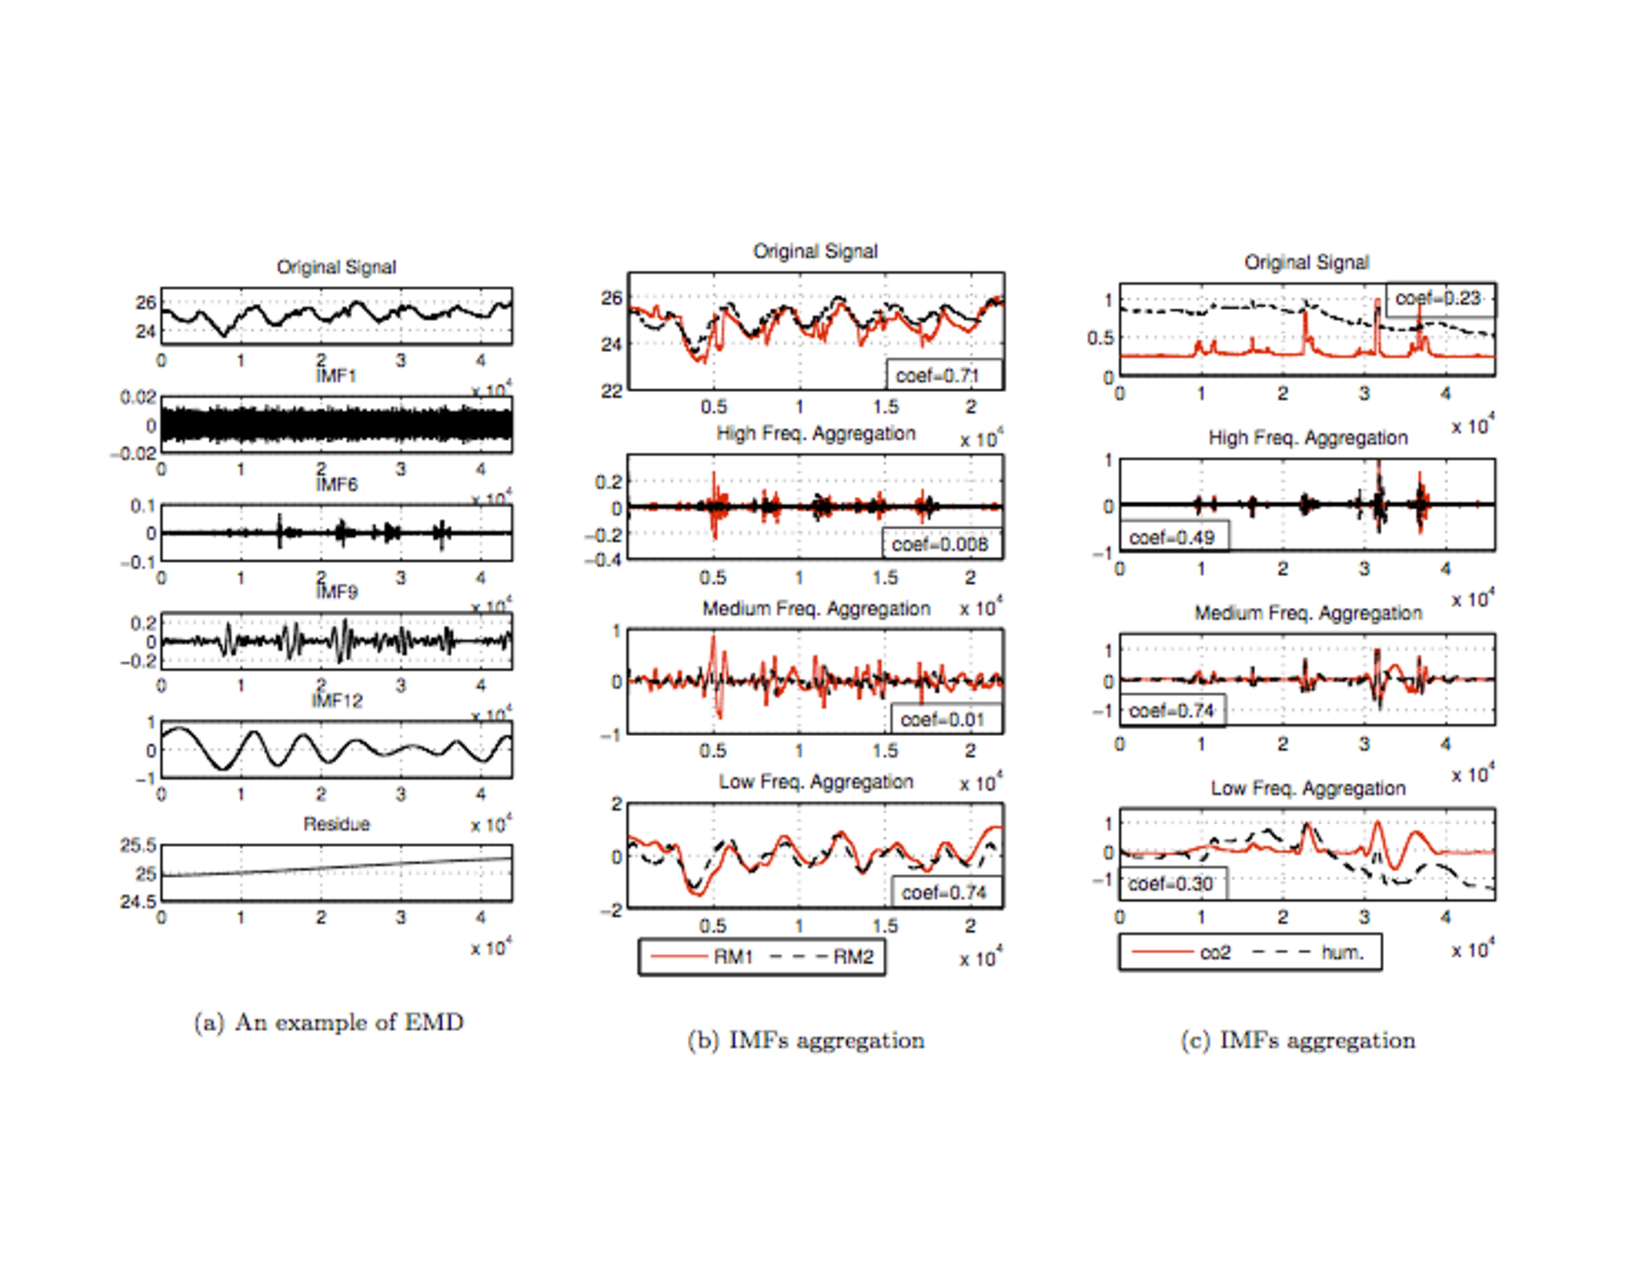
\includegraphics[width=0.95\textwidth]{figs/IMFReAggExample}
\caption{(a) EMD decomposes a signal and exposes intrinsic oscillatory components; (b) Aggregation of IMFs within a pre-defined frequency range makes seemingly similar signals from different locations more distinguishable; (c) IMF aggregation makes seemingly distinct signals of different sensors in the same room show high correlation.}
\end{figure*}

\subsection{Methodology}
We start our analysis by extending the methodology used in SBS~\cite{SBS}, based on empirical mode decomposition (EMD).  
In our analysis, we collect traces from several sensors and run EMD on them.  This produces a set of 
constituent sub-signals called ``intrinsic mode functions'' (IMF), which we separate by frequency range and re-aggregate into distinct bands.
Then, we inspect the relationship between the sensors by computing the corrcoeff within a particular band, which 
gives us the spatial information we are interested in. 
Finally, we separate the result set into sub-sets, and closely examine their statistical characteristics. 
Before describing our methodology in detail, we introduce some definitions and notation.



\subsection{Correlation}
We make extensive use of the correlation coefficient function defined as: 

\begin{displaymath}
r(X,Y) = r_{X, Y} = \frac{\sum_{i=1}^{n} (X_{i} - \overline{X})(Y_{i} - \overline{Y})}
{\sqrt{\sum_{i=1}^{n} (X_{i} - \overline{X})^2}\sqrt{\sum_{i=1}^{n} (Y_{i} - \overline{Y})^2}}
\end{displaymath}

where $X$, $Y$ are separate sets of values, $n$ is the total number of sample points in 
each set, and $\overline{X}$ is the mean value of $X$ (same for $\overline{Y}$ and Y).  % over the entire sampling period.
For each pair of sensors, we compute the corrcoeff to ascertain the relationship between them.


\subsection{EMD Basics}
Non-stationary signals refer to those whose frequencies change over time.  The data generated in buildings is naturally non-stationary, since 
physical readings are highly influenced by the dynamics of physical properties in the immediate surroundings of the sensor.  
 Empirical mode decomposition \cite{EMD} is a method designed for non-linear, non-stationary signal analysis.  We use it to detrend our 
 sensor data and re-aggregate output components within a specific frequency band, based on the SBS methodology~\cite{SBS}. We give a quick overview of EMD and present observations from our data analysis to show a threshold for discovering the boundary between sensor feeds.

\begin{algorithm}[h!]
 \SetAlgoLined
 Give signal $X(t)$:\\
  \While{the \# of maxima in $X(t)$ >3}{
  (1) identify all the local extrema in $X(t)$\;
  (2) perform a cubic spline interpolation of maxima to get the upper envelope\;
  (3) repeat (2) on minima to get the lower envelope\;
  (4) $h(t) = X(t) - mean((2),(3))$ \;
  (5) repeat (2)-(4) until $h(t)$ is an IMF\;
  (6) $X(t) = X(t) - h(t)$, and return the IMF\;
  }
 \caption{Empirical Mode Decomposition}
 \label{alg:emd}
\end{algorithm}

EMD is similar to Fourier transform (FT).  However, for FT to be useful the system (or signal) must be linear and the data must 
be strictly periodic or stationary.  In contrast, EMD directly extracts components associated with different energy from the signal 
and generates a collection of intrinsic mode functions at different time scales.  IMFs are extracted locally and 
normalized to fluctuate around zero.  An IMF is a function with equal number of extrema 
and zero crossings (or differ by one at most), with its envelopes being symmetric with respect to zero.  A summary of the process of 
EMD is depicted in Algorithm~\ref{alg:emd} and the 
reader is referred to~\cite{EMD} for further reading on EMD.  The number of IMFs depends on the original signal and is automatically determined
by a pre-determined stoppage criteria.

\subsection{Re-aggregation}\label{sec:aggr}
In Figure~\ref{fig:emd}, we present example of IMFs extracted using EMD. The original data is generated by a thermometer during a week deployed in a classroom in our testbed building.  The graphs following show the result of the decomposition and re-aggregation methodology in SBS~\cite{SBS}
on this signal.
EMD is able to extract the predominant diurnal pattern (IMF12), induced by occupant activity, from the signal and separate 
distinct flows (IMF9) from other components.  
EMD yields distinct components in different time scales and we compute the instantaneous frequencies \cite{IF} of IMFs using Generalized Zero-Crossing \cite{GZC}. We break the time scales into four frequency bands:
\begin{itemize}
\item High Frequency: a time scale smaller than 30 minutes, mainly reflecting the operation characteristics of devices and noise in system. 
\item Medium Frequency: a time scale between 30 minutes and 6 hours, which is within the time span of daily activities inside a building.
\item Low Frequency: a time scale between 6 hours and 7 days. %This category usually captures patterns repeated in a longer cycle, say, days. 
\item Residue: everything has a time scale longer than 7 days and shows long-term patterns, such as seasonal changes.
\end{itemize}
Figure~\ref{fig:aggr1} shows a comparison of two temperature sensor feeds from different rooms and their respective
decomposition.  Despite strong correlation in the raw time series, the medium frequency IMF shows little correlation.
Only the low frequency diurnal pattern is correlated.  Alternatively,  Figure~\ref{fig:aggr2} shows a $CO_{2}$ trace and a humidity trace.

While the raw signals appear to be very different, and indeed have modest correlation, the medium frequency components
are strongly correlated.  We conjecture that the medium frequency band ``records'' local activity.  Occupants
and movement in the space affect the levels of various physical phenomenon, namely temperature, humidity, $CO_{2}$ levels, etc.
Over shorter time spans, noise in the system hides the effects of local activity.  Longer time-spans capture long-term trends 
related to weather or building operation schedules.  The medium frequency band
captures activities such as meetings and office occupation times.  
These examples illustrate the basis for an automated process.  By isolating a particular component of the signal
we seek to strip away common diurnal factors and also eliminate differences in the response of various sensors to environmental factors.
We combine this observation with a simple classifier to derive colocation.

\subsection{Distribution}
Let $ts^{i}_{j,t}$ be a time-series for sensor $j$ in room $i$ observed over some time interval $t$.  For simplicity, we ignore
$t$ in defining subsequent functions and re-introduce it where necessary.
For each trace we run EMD and obtain a set of $n$ IMFs, denoted as follows:
 % and applying EMD on such a trace will produce,
\begin{displaymath}
\Phi^i_j = EMD(ts^i_j) = \left \{ IMF_{1\sim n} \right \}
\end{displaymath}

IMFs are traces themselves, so we divide and re-aggregate them into the four bands, $B$,
further described in Section~\ref{sec:aggr}.
\begin{displaymath}
B = \left \{ H(igh), M(edium), L(ow), R(esidue) \right \}
\end{displaymath} 

Let the re-aggregation of the bands be denoted as:
\begin{displaymath}
Aggr(\Phi^i_j) = \left \{ IMF^i_{f,j} \right \}
\end{displaymath} 

where $f \in B$.  We pick the \emph{medium} frequency band ($M$) to compute the pairwise corrcoeff of the sensor traces. 
In order to understand and characterize the boundary between sensors we consider two sets of corrcoeffs for each room; the ``intra"-room set and 
``inter"-room set, as defined:
\begin{displaymath}
R^{i}_{intra,t} = \left \{ r(IMF^{i}_{M,j,t}, IMF^{i}_{M,k,t}) \right \}, \,
s.t.\, \forall j,k \in S_i
\end{displaymath}

The intra set only contains pairs of sensors in the same room, so both $ts^{i}_{j,t}$ and $ts^{i}_{k,t}$ are traces from 
sensors in room $i$.
\begin{displaymath}
R^{i}_{inter,t} = \left \{ r(IMF^{i}_{M,j,t}, IMF^{i'}_{M,k,t}) \right \},
\end{displaymath}
\begin{displaymath}
s.t. \, \forall j \in S_i, \, \forall k \in S_i', \, i \neq i' 
\end{displaymath}

By contrast, the \emph{inter} set contains pairs across rooms, meaning $ts_{j,t}$ is a trace from a sensor in room $i$ and 
$ts_{k,t}$ is a sensor trace from some other room $i'$.  %, and $t$ is the time span of the sensor trace the IMFs are derived from.
Note the use of $t$ in the definitions.  We re-introduce $t$ here to denote that the construction of each set is performed with respect to a specific time interval.

Finally, we examine populations, $R^i_{intra}$ and $R^i_{inter}$, across multiple time intervals (in days):%which are defined as,
\begin{displaymath}
R^{i}_{intra} = \bigcup_{\forall t}^{} R^i_{intra, t}, \; s.t. \; t \in \left \{ 1,3,5,7,14,21,28\right \}
\end{displaymath}

\begin{displaymath}
R^{i}_{inter} = \bigcup_{\forall t}^{} R^i_{inter, t}, \; s.t. \; t \in \left \{  1,3,5,7,14,21,28\right \}
\end{displaymath}

We generate a CDF for each of the two populations with respect to each room.  
This allows us to closely examine the statistical characteristics 
of the relationship between sensors in the same space and those in different spaces.  Each room offers a potentially different 
perspective on this relationship.


\subsection{Threshold Analysis}
In order to understand the statistical properties, we generate two corrcoeff distributions by computing the corrcoeff between pairs of traces within and across each room, as detailed in the previous section.
Figure~\ref{fig:group} shows how we divide the corrcoeff values into two sets.
The figure shows two intra and two inter sets. Specifically, we examine how a choice in cut-off threshold affects the ability
to separate the sets, when their separation is not known a priori, relative to each room.
Our hypothesis is that there exists a computable, statistical boundary between sensors in different rooms.

To test our hypothesis, we choose a threshold value relative to the distribution of corrcoeffs.  
All pairs with a corrcoeff larger than the threshold will be classified as being in the same room.  To closely analyze the threshold parameter, 
we generate a receiver operating characteristic (ROC) curve by varying the threshold value.  Then, we look for a good tradeoff point between the true-positive and false-positive rate; one that maximizes the difference between TPR and FPR.  We compare the ROCs generated 
for our ``medium'' frequency band IMFs against raw-signal, cross-correlation values, in order to ascertain the extent to which 
the SBS~\cite{SBS} methodology is advantageous for discovering a statistical separation, analogous to a physical one.
We also examine whether there is a uniform boundary between clusters across all the rooms. 


\begin{figure*}[ht!]
\centering
	 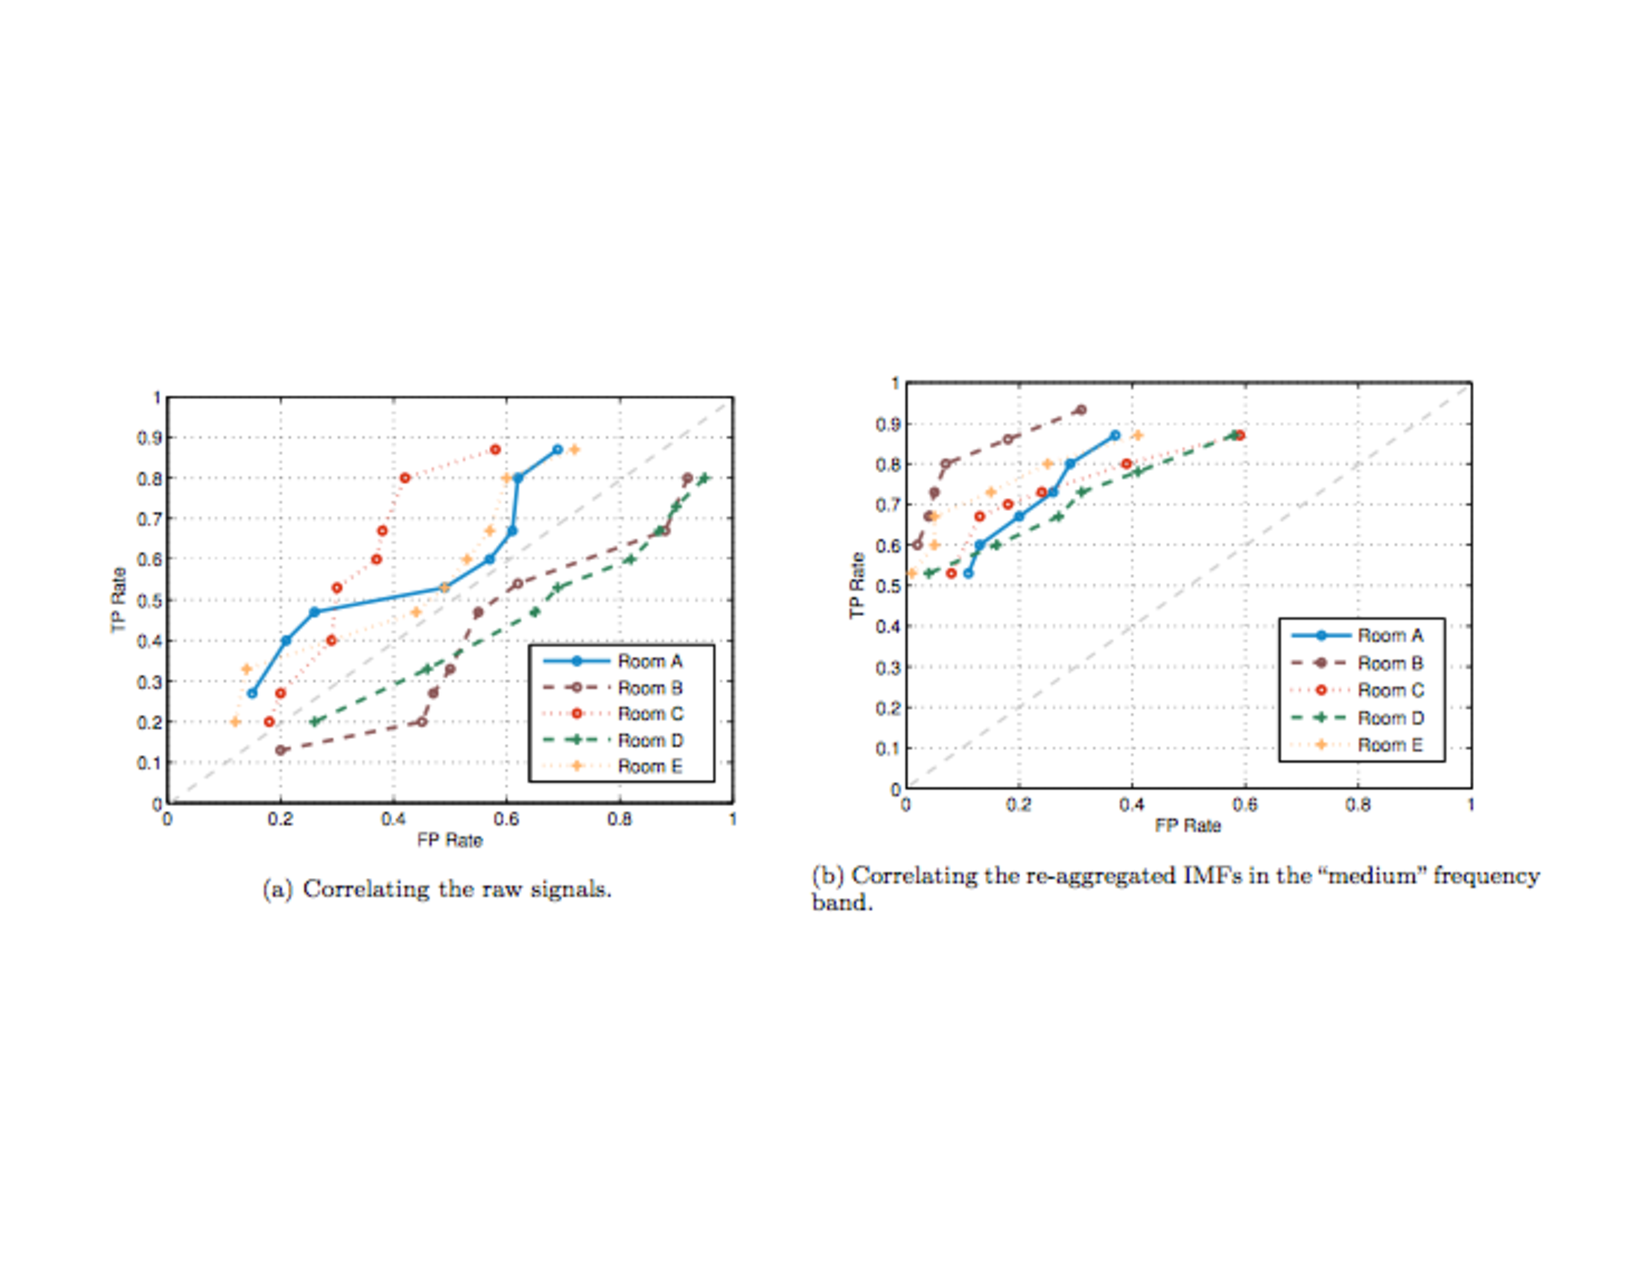
\includegraphics[width=0.95\textwidth]{figs/ROCgraphs}
\caption{The ROC curves depict the sensitivity of the raw signal and mid-frequency IMFs to the threshold value. We choose the 0.2 FPR point as the boundary threshold for each room. }
\label{fig:roc}
\end{figure*}

\section{Spatial Clustering Experimental Results}
We conduct two sets of experiments. First, we quantify the sensitivity of our method for different threshold values 
and examine the effect of different time spans on the threshold. We then cluster the traces based on our threshold analysis 
and compare it with a baseline approach using multidimensional scaling and k-means.
% as well as with an approach combining multidimensional scaling and k-meas. 
% Last, we validate the usefulness of the proposed method in a case study.

\subsection{Experimental Setup}
\begin{figure}[h!]
\centering
  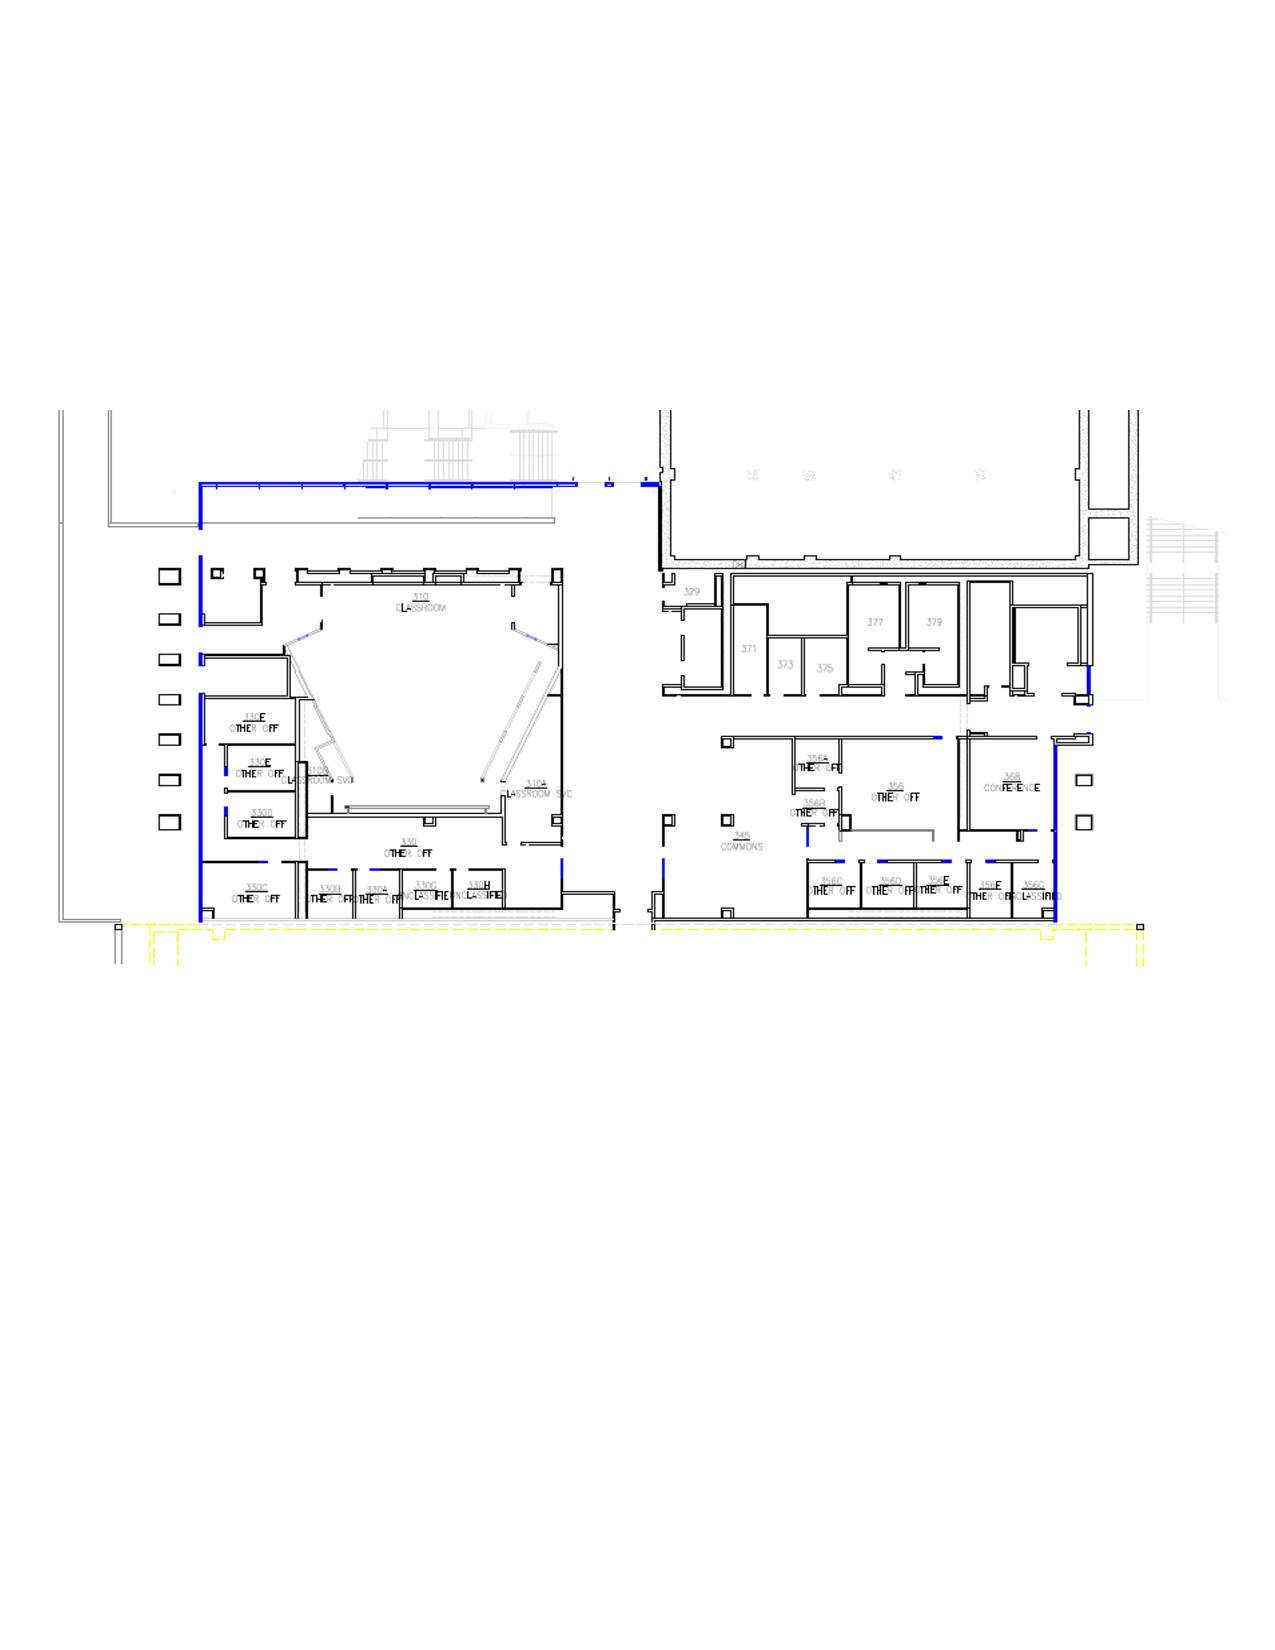
\includegraphics[width=0.45\textwidth]{figs/SDH3_crop}
\caption{We collect data from 15 sensors in 5 rooms sitting on 4 different floors. This is a map of a section of the 3rd floor
in Sutardja Dai Hall.}
\label{fig:sdh}
\end{figure}

We perform an empirical study on sensor data collected from 15 sensors across 5 rooms on 4 different floors of a large building, as detailed in Table~\ref{table:roomspec}. 
Each room has three sensors: a temperature sensor, a $CO_{2}$ sensor,  and a humidity sensor. 
The data from these is reported to an sMAP~\cite{smap} archiver. The data set used comes from a deployment~\cite{Jay} lasting 
over 6 months on several floors in Sutardja Dai Hall (SDH) at UC Berkeley, where one sensor box -- which contains a thermometer, a humidity sensor and a $CO_{2}$ sensor -- is placed in each room. The box reports data over 6LowPAN~\cite{6lowpan} to a sMAP archiver every 15 seconds. 
 % The other is a long-term deployment comprised of thousands of sensors that are part of the Building Management System (BMS).
 % We choose the portion of the SDH data set where the sensor devices, accessible via BACnet~\cite{BACnet}, report data to the archiver every 
 %few minutes. 
 Due to intermittent data loss, we pick a time span without interruption, starting in January until mid-Feburary, 2013, for evaluation.

\begin{table}[ht!]
\caption{Room Specs}
\centering % used for centering table
\begin{tabular}{c c c c}% centered columns (4 columns)
\hline %inserts single horizontal lines
Room\# & Orientation & Floor & Type \\ % inserts table 
%heading
\hline\hline % inserts double horizontal line
A & West & 2 & Computer Lab \\ % inserting body of the table
B & South & 4 & Conference Room \\
C & No Window & 2 & Classroom \\
D & North & 7 & Conference Room \\
E & South & 5 & Conference Room \\ % [1ex] adds vertical space
\hline %inserts single line
\end{tabular}
\label{table:roomspec} % is used to refer this table in the text
\end{table}

\subsection{Baseline and Metrics}
% We exploit a simple approach as baseline to compare with our proposed approach: instead of computing the correlation coefficients between re-aggregated IMFs of sensor feeds, we directly use the raw sensor data to do the correlation analysis and generate the two distributions for thresholding approach evaluation similarly to what described previously.

% As a baseline, we perform correlation analysis on the raw data. We generate two distributions, as previously described, and observe the effects of the choice of threshold on the true/false positive rate.
As a baseline, after we generate the two distributions described previously, we apply multidimensional scaling (MDS) to the corrcoeff matrix, in order to transform the original high-dimensional relative space to a 3-D space with an absolute origin, and run the k-means clustering algorithm.
We choose the true-positive rate (TPR, also known as recall rate) and false-positive rate (FPR) as metrics to evaluate the performance of our method versus the naive approach, which correlates the raw traces. A true-positive (TP) is when a sensor pair in a room is classified as being co-located 
while a false-positive (FP) is when a sensor that is not in room is classified as being so.
%is that a sensor not in room A is clustered as in room A.

\begin{figure}[h!]
\centering
	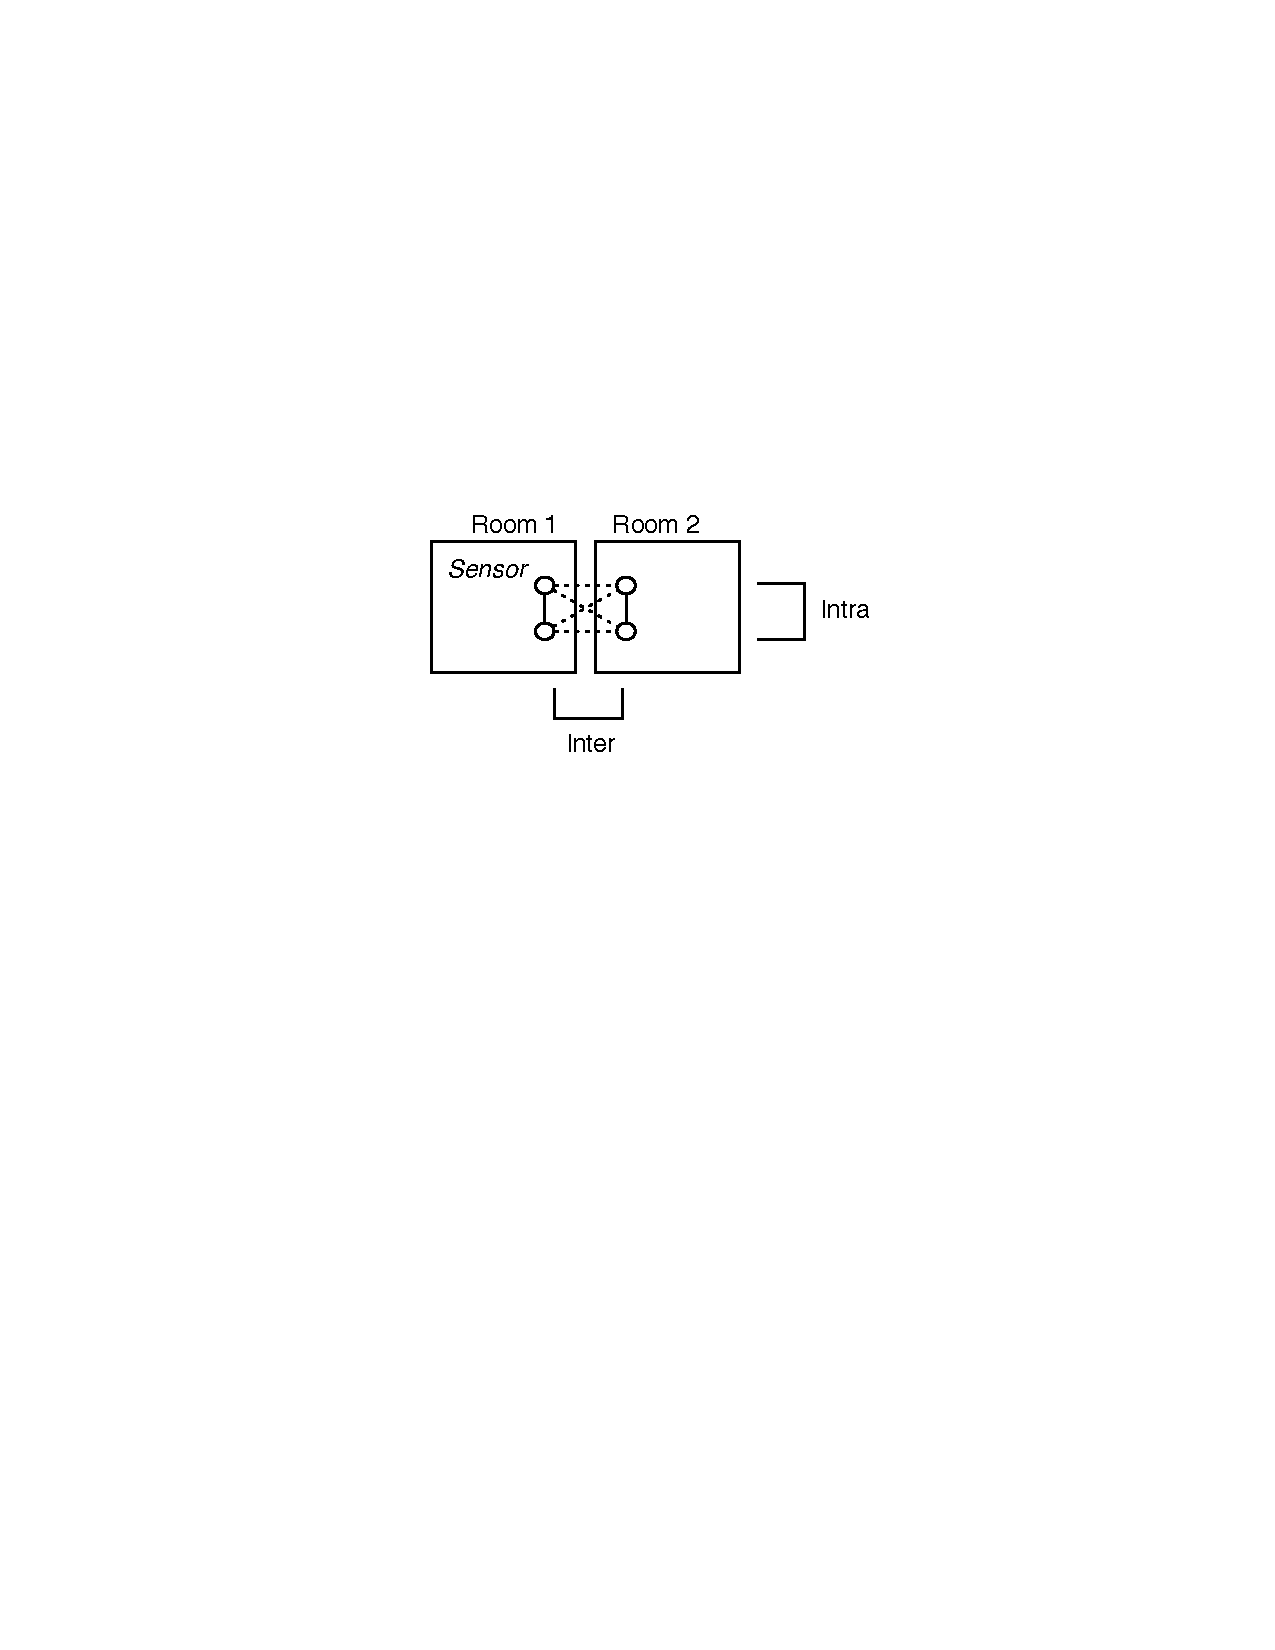
\includegraphics[width=0.45\textwidth]{figs/Inter_intra_relationships}
\caption{Two populations are examined for our threshold analysis.  A solid line connects sensors in the same room while a dotted line connects
 to a pairs in different rooms.}
\label{fig:group}
\end{figure}

\begin{figure}[h!]
\centering
	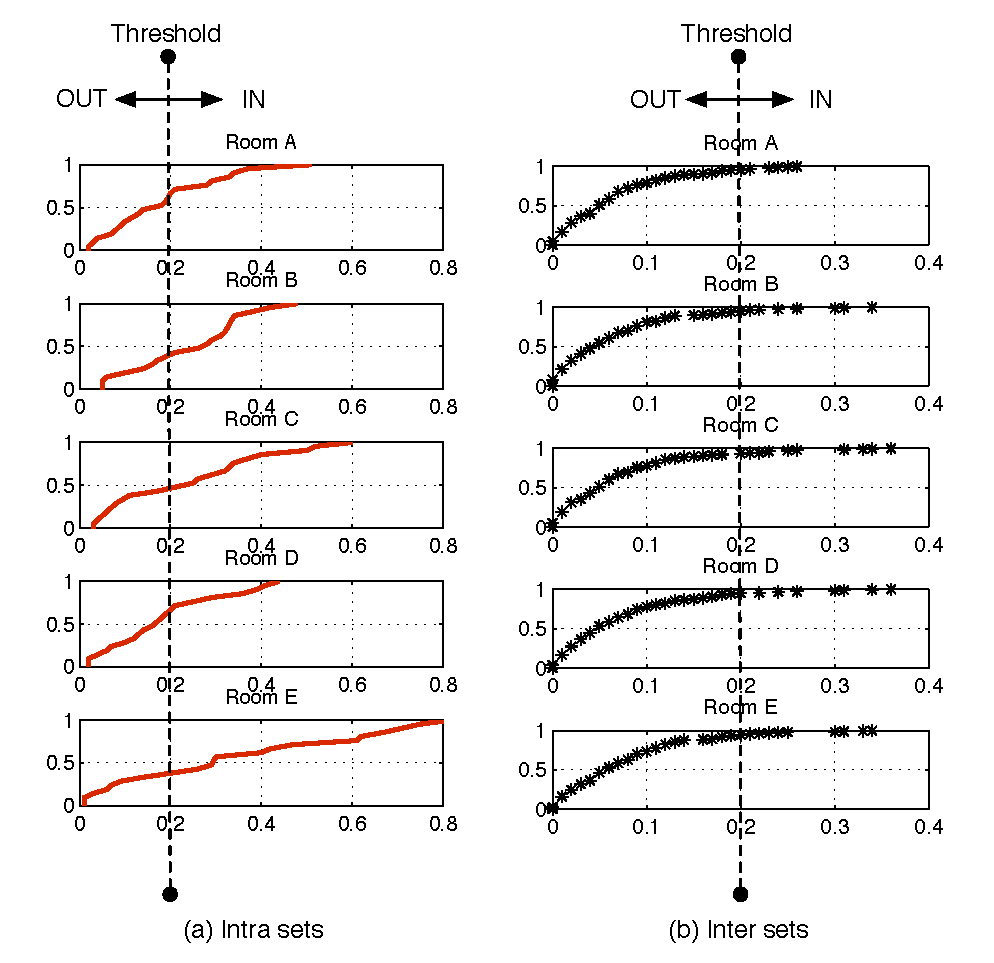
\includegraphics[width=0.45\textwidth]{figs/corrcoeff_cdf_in_out}
\caption{CDF of correlation coefficients between IMFs of sensor feeds: the dotted lines point to some threshold which divides
 the distribution and produces a TPR and FPR.
}
\label{fig:cdf}
\end{figure}

\subsection{Characterizing the Boundary}
To corroborate our boundary-existence hypothesis, we first need to characterize the boundary between sensors in different rooms. 
We compute the pairwise correlation coefficients (corrcoeffs) between sensor traces in both of populations depicted in Figure~\ref{fig:group}, 
over different time spans -- ranging from one day to one month.
After generating points over different time 
spans for each room, we accumulate the corrcoeffs to obtain distributions as shown in Figure~\ref{fig:cdf}, for each of the five rooms. 

The dashed vertical lines in Figure~\ref{fig:cdf} 
represent an arbitrary threshold that partitions the distribution into two sets.  Pairs of sensors to the right of the line
are classified as being in the same room.  Pairs of sensors to the left are classified as being in different rooms.
The CDFs on the left column show the distribution of corrcoeffs for pairs known to be in the same room and the CDFs on the right
show the distribution of corrcoeffs in different rooms.
Note in the figure, we set the threshold to the same value to both the left and right side, in order to observe the effect of the true/false positive
rates.
By adjusting the threshold, we get different TPRs/FPRs parameterized by the threshold. Figure~\ref{fig:roc} captures the range tradeoff in a corresponding ROC curve.


Figure~\ref{fig:roc} illustrates the TPR/FPR sensitivity to different threshold values for our method and the naive approach. A good cluster achieves a high TPR and a low FPR. 
As we vary the threshold, we see that our approach 
achieves a TPR between 52\%--93\% and a FPR between 5\%--59\%.  %The baseline, mostly remains along the diagonal, meaning it is practically random. 
We can see that the average TPR for the ROC graph on the right is higher than the 
ROC graph on the left.  Moreover, the corresponding average FPR is lower on the right than on the left.
In general, as the TPR rises, the FPR also goes up -- \emph{a tradeoff exists between maximizing TPR and maintaining a lower FPR}.


 The ``boundary'' is represented as the corrcoeff that produces a ``good" TPR with an ``acceptable" FPR.  In Figure~\ref{fig:rocA}, 
  we choose 0.2 FPR as the boundary threshold.  This point represents the largest difference between TPR and FPR -- an acceptable tradeoff point. 
Looking at Figure~\ref{fig:cdf}, the 0.2 FPR corresponds roughly to the 80th-percentile correlation coefficient, on the ``inter''
set (the set of CDFs on the right).
  The recall rate for each room -- using a 80th-percentile corrcoeff threshold value -- ranges between 62\%-86\% and the 
  threshold value falls into a narrow interval between 0.1 to 0.12. This shows that \emph{we are able to choose a uniform value 
  for all the rooms regardless of the sensor type.}

\subsection{Convergence over Time}
\begin{figure}[h!]
\centering
	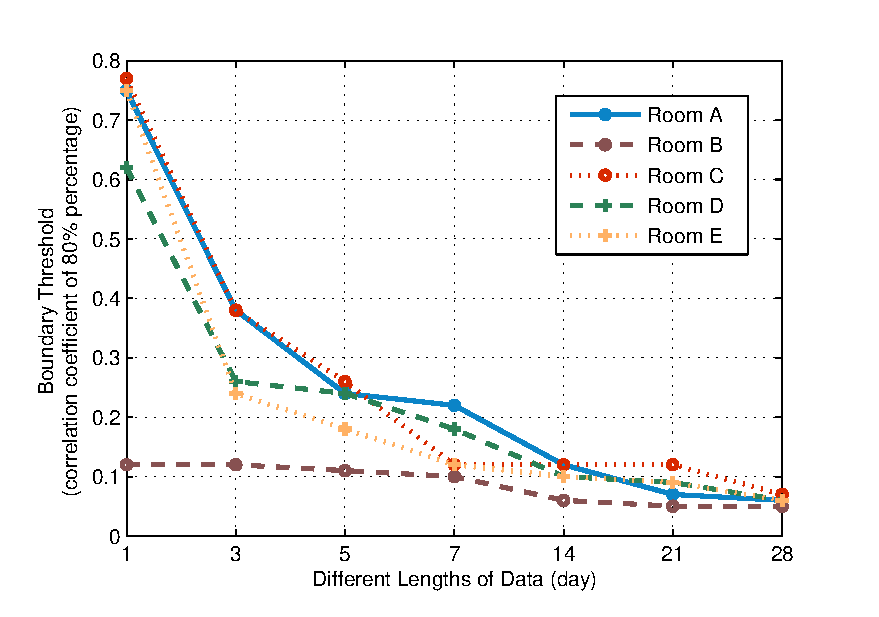
\includegraphics[width=0.48\textwidth]{figs/lengtheffect.eps}
\caption{The threshold values all converge to a similar value and we can derive the optimal value with as minimal as 14 days data.}
\label{fig:leneff}
\end{figure}

Using the threshold the roughly 80th-percentile corrcoeff corresponds to in the distribution, we examine how it affects the classification rate across traces
that span different lengths of time.  Convergence and consistency across different time spans is critical to automate the parameter selection
process.
Observe how the  threshold values differ quite significantly in Figure~\ref{fig:leneff}.  However, 
the threshold values 
gradually converge, as the length of training data increases from one day to one month.  The values derived after 14 days of data
are approximately the same as the final convergence value (around 0.07).  In other words, we can determine a threshold from two weeks of data.

\subsection{Clustering Results}
We cluster the sensor traces over the entire one-month period, and use the roughly 80th percentile corrceff (0.07) as the boundary threshold. 
A sensor is classified into the cluster with the largest corrcoeff. The clustering result is shown in Table~\ref{tab:cluster}.  A ``1" means the sensor is classified as inside the corresponding room. 
In general, after obtaining the sensor clusters, we don't know which room each cluster corresponds to without further information such as the metadata of sensors. The labels ``A-E" in Table~\ref{tab:cluster} are used to indicate the ground truth of where each sensor is physically placed since we have such information. Overall, the classification accuracy 
is 93.3\%.  We do not cluster on the corrcoeffs obtained among raw signals because the 80\%-percentile corrcoeff values do not converge across rooms.
The reason that we are able to get such a high accuracy, which is seemingly different from the statistics in Figure~\ref{fig:cdf} and Figure~\ref{fig:roc}, is because the statistics in the two figures are generated out of the corrcoeffs accumulated over different time spans (the same intervals in Figure~\ref{fig:leneff}) while the clustering here is performed on the corrcoeffs from the entire one-month period. 
% vary a lot and it doesn't make much sense to use different threshold for each room individually.

\begin{table}[h!]\footnotesize
 \begin{center}
	\begin{tabular}{ r|c|c|c|c|c|c }
	\multicolumn{1}{r}{}
	 &  \multicolumn{1}{c}{$A$}
	 & \multicolumn{1}{c}{$B$}
	 & \multicolumn{1}{c}{$C$}
	 & \multicolumn{1}{c}{$D$}
	  & \multicolumn{1}{c}{$E$} \\
	\cline{2-6} 
	$SensorA_{1}$ & 1 & 0 & 0 & 0 & 0 & \checkmark\\
	\cline{2-6}
	$A_{2}$ & 1 & 0 & 0 & 0 & 0 & \checkmark\\
	\cline{2-6}
	$A_{3}$ & 1 & 0 & 0 & 0 & 0 & \checkmark\\
	\cline{2-6}
	$B_{1}$ & 0 & 1 & 0 & 0 & 0 & \checkmark\\
	\cline{2-6}
	$B_{2}$ & 0 & 1 & 0 & 0 & 0 & \checkmark\\
	\cline{2-6}
	$B_{3}$ & 0 & 1 & 0 & 0 & 0 & \checkmark\\
	\cline{2-6}
	$C_{1}$ & 0 & 0 & 1 & 0 & 0 & \checkmark\\
	\cline{2-6}
	$C_{2}$ & 0 & 0 & 1 & 0 & 0 & \checkmark\\
	\cline{2-6}
	$C_{3}$ & 0 & 0 & 1 & 0 & 0 & \checkmark\\
	\cline{2-6}
	$D_{1}$ & 0 & 0 & 0 & 1 & 0 & \checkmark\\
	\cline{2-6}
	$D_{2}$ & 0 & 0 & 0 & 1 & 0 & \checkmark\\
	\cline{2-6}
	$D_{3}$ & 0 & 0 & 1 & 0 & 0 & $\times$\\
	\cline{2-6}
	$E_{1}$ & 0 & 0 & 0 & 0 & 1 & \checkmark\\
	\cline{2-6}
	$E_{2}$ & 0 & 0 & 0 & 0 & 1 & \checkmark\\
	\cline{2-6}
	$E_{3}$ & 0 & 0 & 0 & 0 & 1 & \checkmark\\
	\cline{2-6}
	\end{tabular}
 \end{center}
 \caption{Clustering result using the thresholding method: a ``1" means the sensor is classified as inside the room. We get the ``\checkmark" and ``$\times$" by comparing the clustering results with ground truth.}
 \label{tab:cluster}
\end{table}

\begin{figure*}[ht!]
\centering
	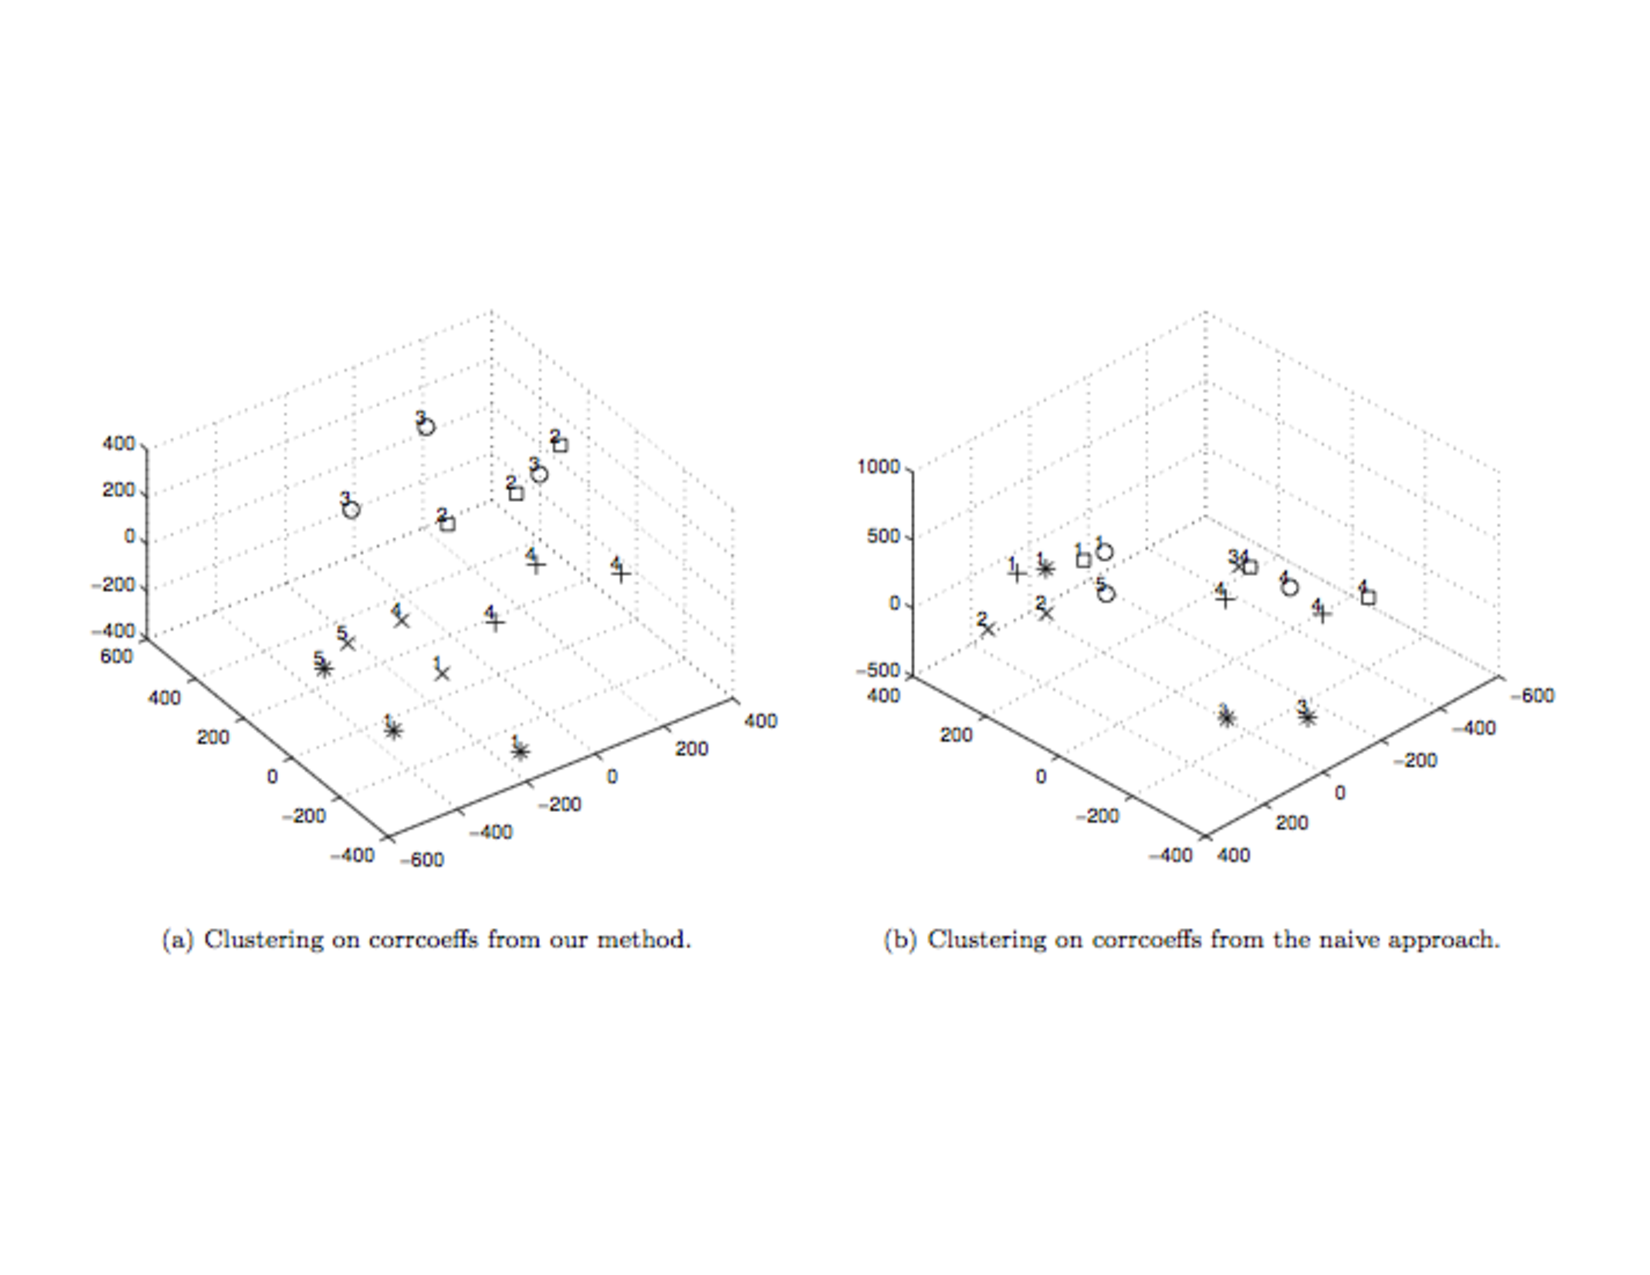
\includegraphics[width=0.48\textwidth]{figs/Space_KmeanClustering}
\caption{Clustering with k-means on the corrcoeff matrix after applying multidimensional scaling (MDS): The EMD-based set achieves an accuracy of 80\% while the results with raw-trace is only 53.3\% classification accuracy.}
\label{fig:mds}
\end{figure*}

To compare with our threshold-based method, we also cluster using a baseline approach. The pairwise corrcoeff for sensors in different rooms can be interpreted as a ``distance" between them.
A larger coefficient indicates a closer ``distance", and vice versa.  However, since the distances between pairs is relative, we use
multidimensional scaling~\cite{MDS} to find a common basis in three dimensions, re-map the relative distance metric (feature vector) into 
this three-dimensional grid and use k-means to classify the traces. % assuming the value of k is known a priori, which is the number of rooms.
We set k to equal the number of rooms, since the goal of the approach is to verify spatial placement at room-level granularity.  Generally, 
we believe that k should equal the number of rooms you wish to classify the sensors into. 
The clustering results are shown in Figure~\ref{fig:mds}.  Ground truth is shown through different markers (x, o, +, star, box). Each marker stands for one room. 
The cluster each sensor assigned to is denoted with a number. The classification accuracy of the baseline approach on corrcoeffs matrix of re-aggregated IMFs is 80\%. 
For raw traces, the baseline approach achieves an accuracy of only 53.3\%.

\subsection{Discussion}
\paragraph{Bi-modal Distribution} From the results illustrated in Figure~\ref{fig:cdf}, we observe a bi-modality in the corrcoeff 
distribution for the two population sets.  Sensors in the same room correlate to each other more (typically a corcoeff of 0.4 or higher)
than sensors in different rooms.  % have much smaller corrcoeff values. 
This bi-modal distribution may provide insight for us to 
% lays the foundation for us to 
understand the boundary and search for an effective discriminator more broadly.

\paragraph{Across Different Sources}
To further validate the effectiveness of the proposed method, we should consider using data from different sources.
For example, in room B in Sutardja Dai Hall, there are two different sets of temperature sensors reporting data at different rates and granularities.
We demonstrate our ability to classify sensor streams on the same platform (recall the sensor box we used to collect data). 
It would be more convincing to verify the effectiveness of our method with sensor streams generated from devices on
 different systems -- since separate systems are independent.  For instance, we can use temperature data from the second deployment 
 and use the $CO_{2}$ and humidity sensor data from the first deployment and compare the results to what we have gathered.

\paragraph{Generalizability} In our results, the boundary threshold parameter converges to a narrow interval, as the data set expands 
over a longer time range.  This may suggest that our method generalizes across rooms in a building, although further validation in a 
larger, more representative data set is necessary.  This study looked at 5 different rooms with a large physical separation from one
another.  A more representative data set would consider all the rooms and pay special attention to rooms that share a common orientation
and are separated by a single wall or floor slab.
  
Based on this study, and the previous, related one~\cite{IOT}, we conjecture that local activity modulates various types of physical 
signals -- captured by the various kinds of physical sensors embedded
throughout the building -- and that those signals are attenuated
over distance and physical boundaries (such as walls).  We believe that this is what drives our observations. 
If the conjecture is true, the effects will be less pronounced in larger rooms, such as an auditorium or a large laboratory space.


As our approach performs slightly better than traditional learning techniques, we must further evaluate its robustness
versus the baseline method; across the entire building and across multiple buildings.  In future work, we will examine the 
two approaches across larger intra-building data sets and compare results across multiple buildings.
A key factor is the variance of classification accuracy -- smaller variance demonstrates robustness.  


\subsection{Spatial Verification Take-aways}
We present a new method for spatial placement clustering.  
We first characterize the corrcoef distribution of medium frequencies IMFs between sensors in the same/different room(s), and then we learn the tradeoff between achieving a higher TPR and maintaining a lower FPR by manipulating a discriminator parameter within these two distributions. 
For a preliminary sample of relatively well separated rooms, we find that there is a clear boundary between sensor clusters in terms of their spatial placement and the boundary can be probed statistically.  We also find 
a uniform discriminator can be learned and generalized across these rooms.  
For this initial study, our method is able to classify the sensors of 93.3\% accuracy, which is 13\% higher than a tradition k-means approach, with a TPR between 62\%-86\% and a FPR less than 20\%. 

These results are very encouraging. However, we recognize that they are far from definitive. While the rooms in the study were picked arbitrarily, they are neither comprehensive nor a systematic sampling.  While they are clearly separated by our approach, and not by analyses of the raw time series, they do differ substantially in placement and usage.  A key question going forward is, ``how well will highly similar rooms be separated?"  - say, adjacent rooms facing the same side of the building and with similar occupancy. Will these techniques hold, more powerful techniques be required, or is further discrimination intractable? In future work, we will examine how far this method takes us and explore how it may be used in combination with other techniques to improve the results more generally. Automated metadata verification is important to include in the lifecycle of building data management.

























\section{Type Verification With K-Nearest Neighbors}


\section{Type Verification: Experimental Results}

\begin{figure}[t!] %htbp
\centering
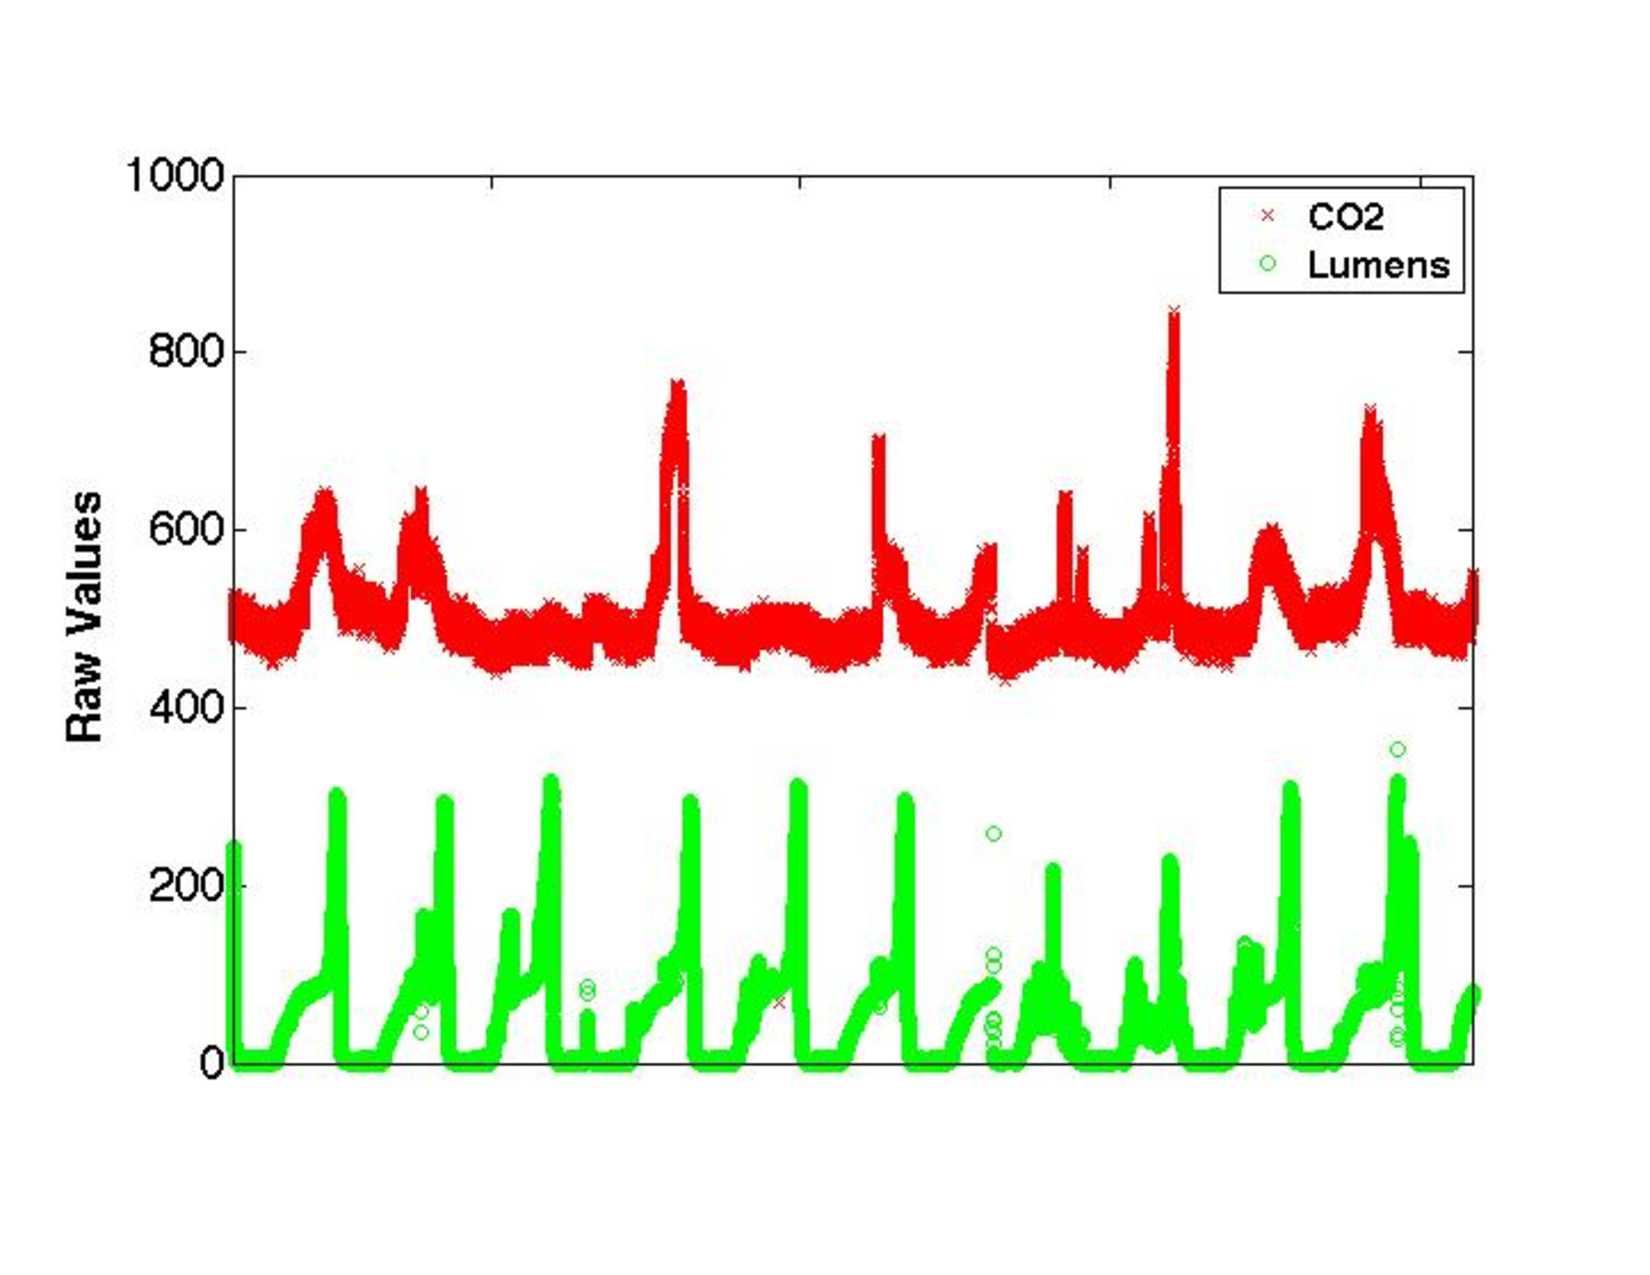
\includegraphics[width=0.75\columnwidth]{figs/KETI413_co2_light_raw}
\caption{}
\label{fig:co2_light_raw}
\end{figure}

\begin{figure}[t!] %htbp
\centering
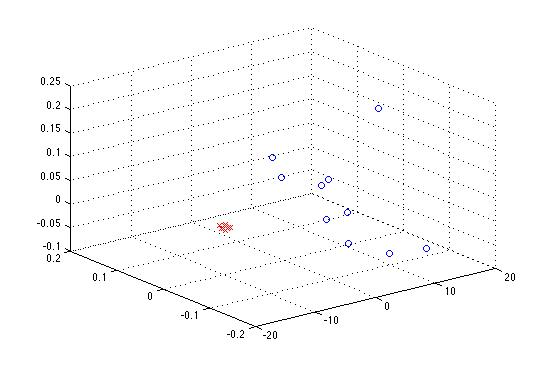
\includegraphics[width=0.75\columnwidth]{figs/EMD_LF_PCA_413_co2_light}
\caption{}
\label{fig:EMD_LF_PCA}
\end{figure}

\begin{figure}[t!] %htbp
\centering
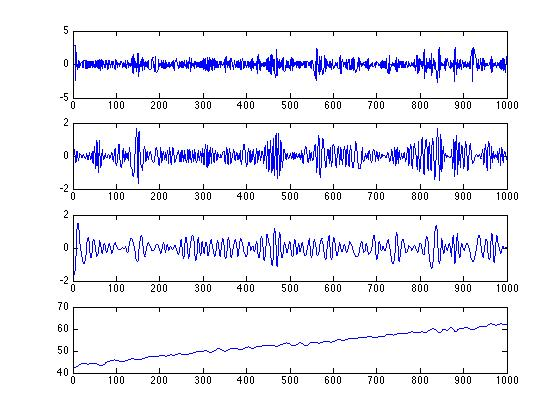
\includegraphics[width=0.75\columnwidth]{figs/KETI413_6h_light_3IMF}
\caption{}
\label{fig:light_3IMF}
\end{figure}

\begin{figure}[t!] %htbp
\centering
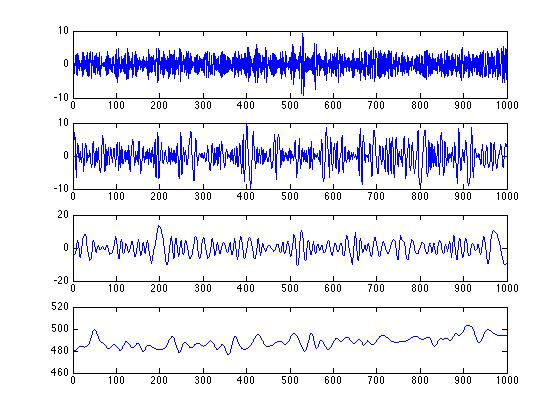
\includegraphics[width=0.75\columnwidth]{figs/KETI413_co2_6h_3IMFs}
\caption{}
\label{fig:co2_3IMFs}
\end{figure}


\begin{figure}[t!] %htbp
\centering
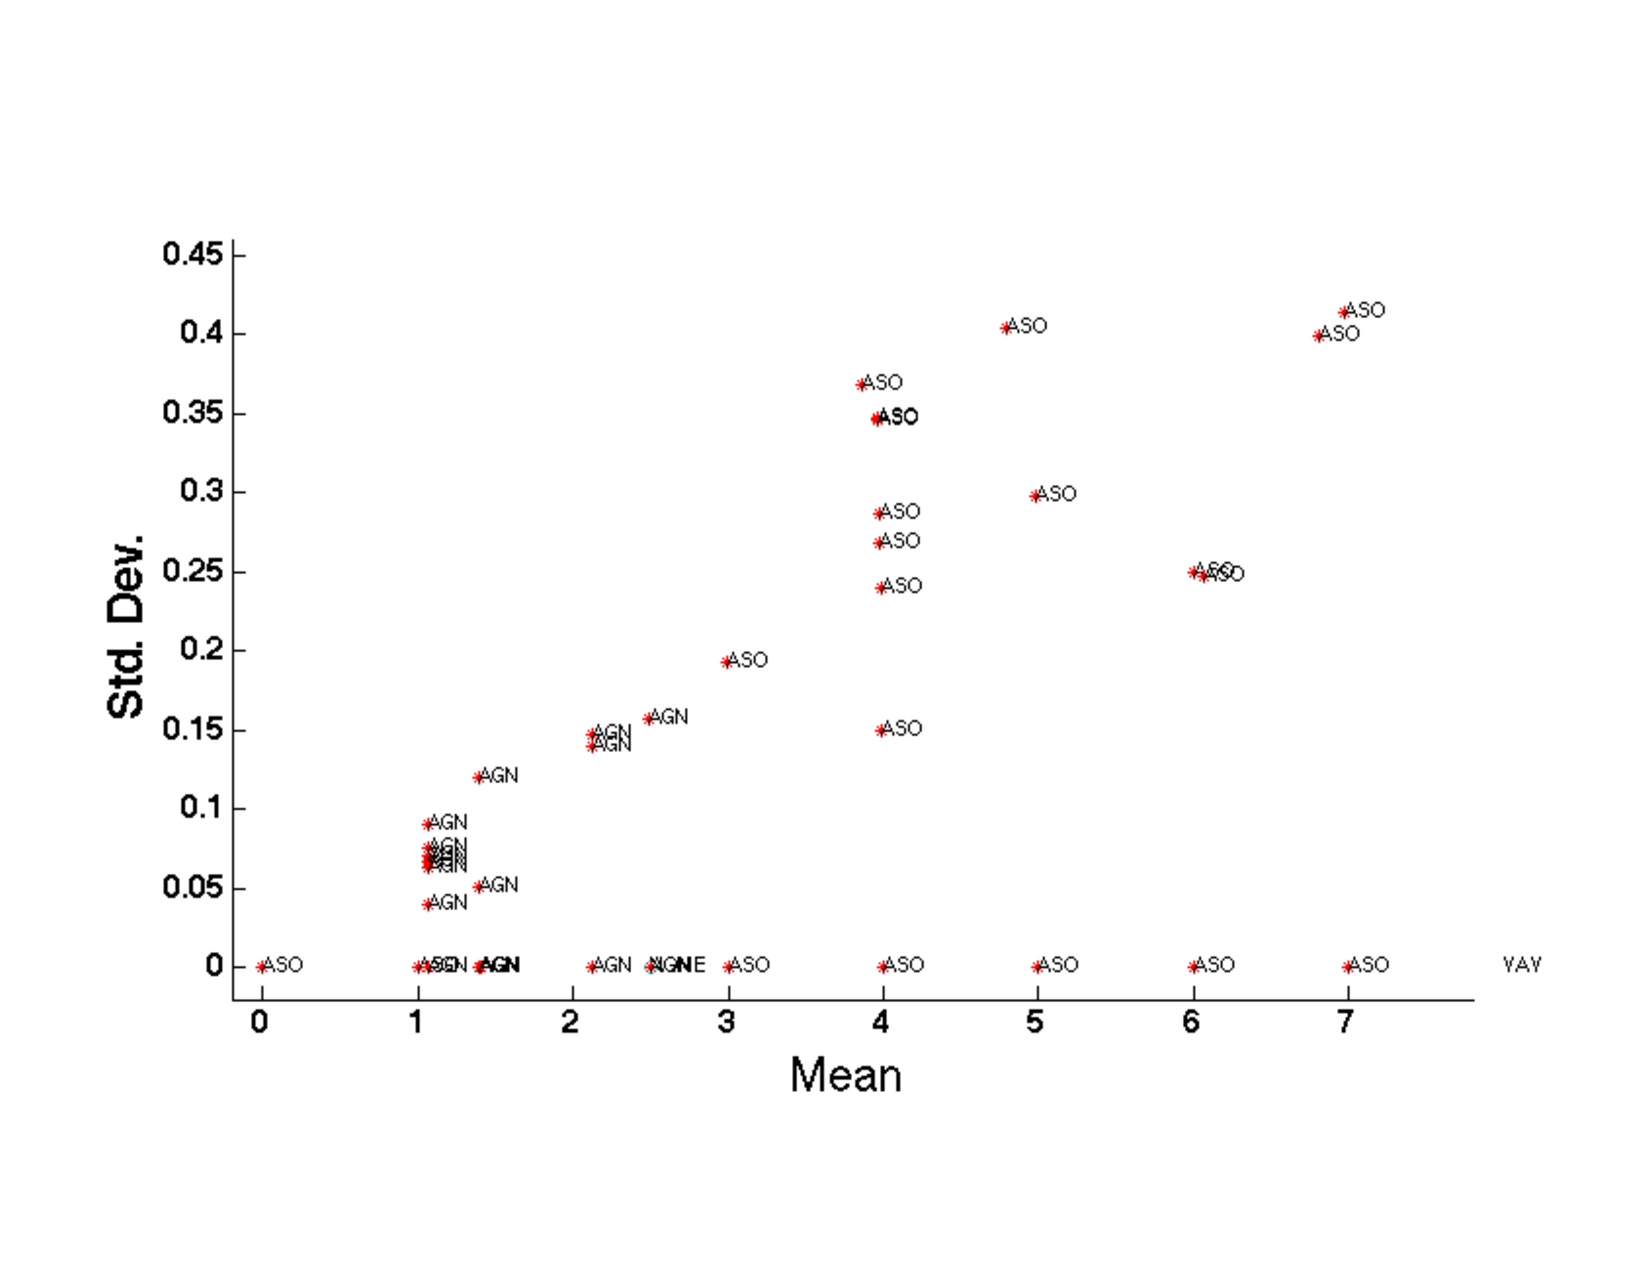
\includegraphics[width=1.0\columnwidth]{figs/ASOvsAGN}
\caption{}
\label{fig:asovsagn}
\end{figure}

\begin{figure}[t!] %htbp
\centering
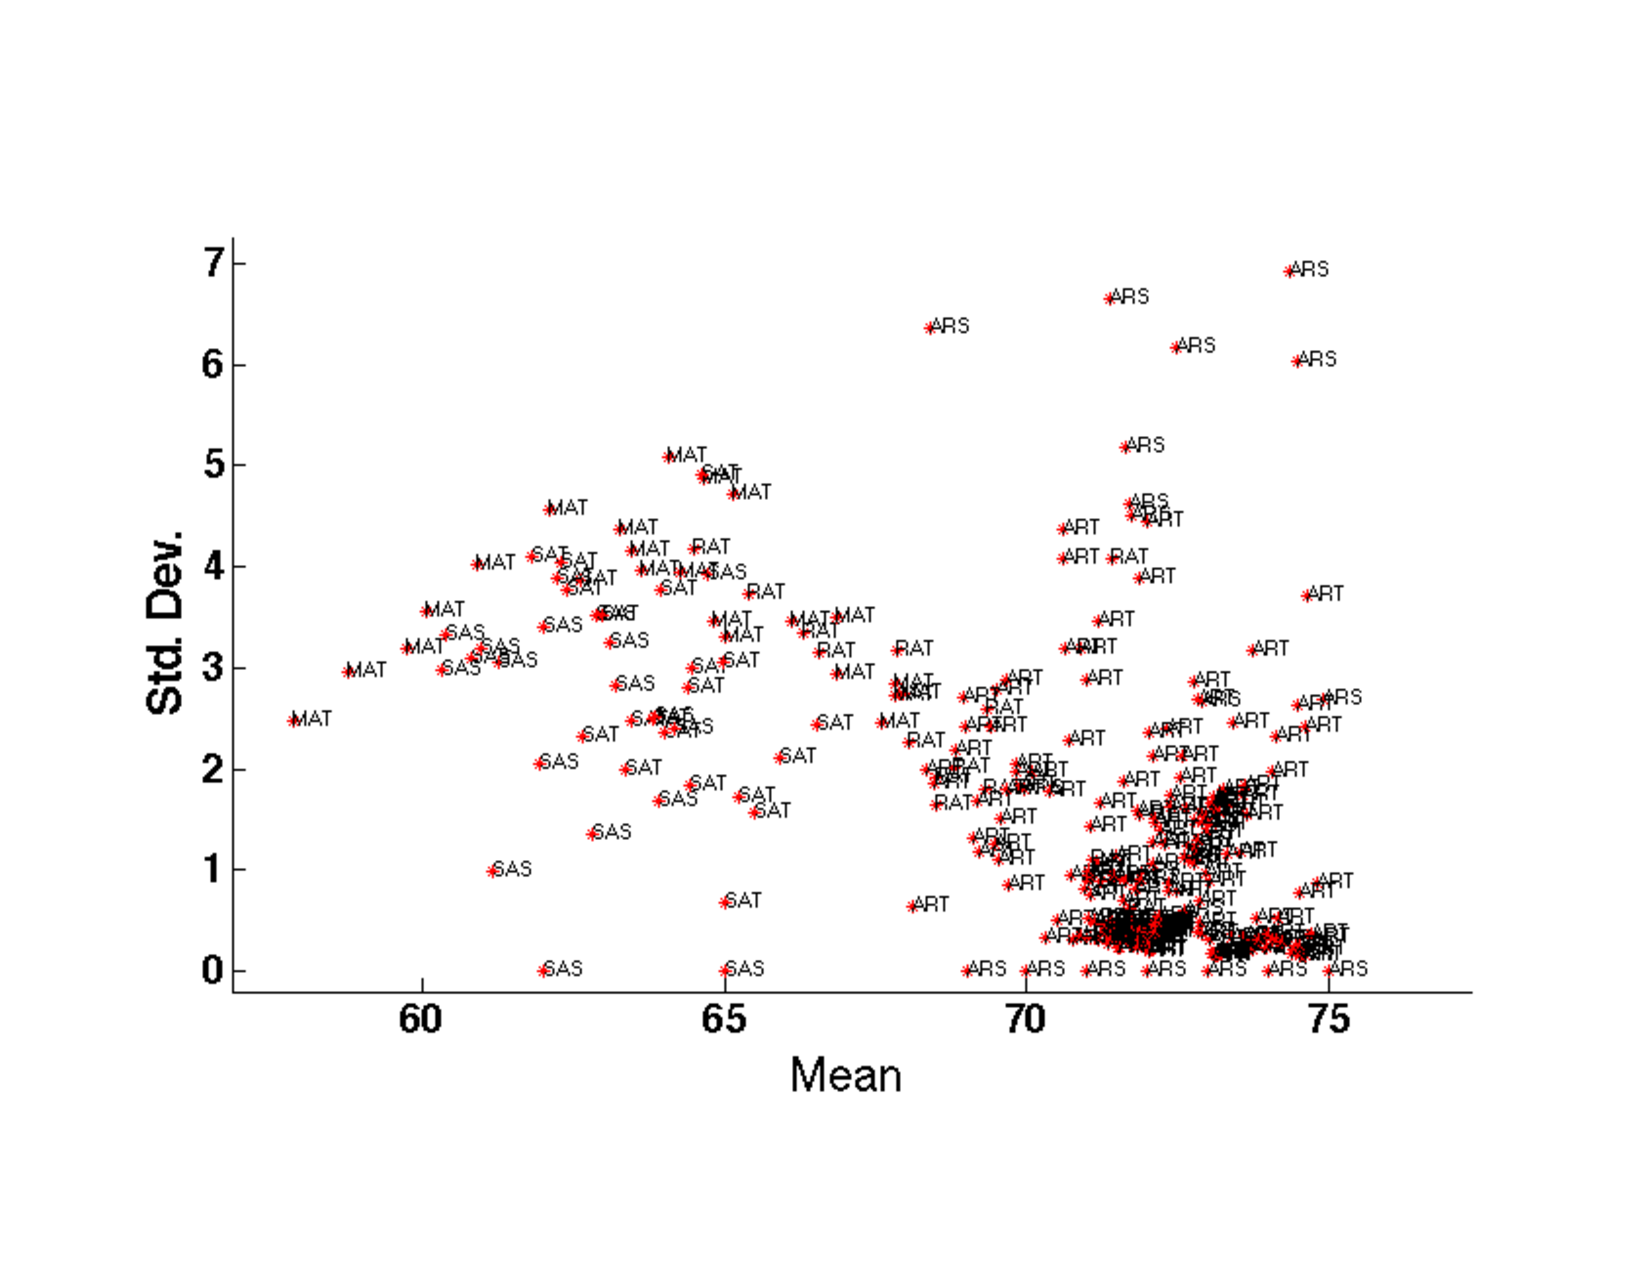
\includegraphics[width=1.0\columnwidth]{figs/temperature_streams}
\caption{}
\label{fig:tstreams}
\end{figure}


\begin{figure}[t!] %htbp
\centering
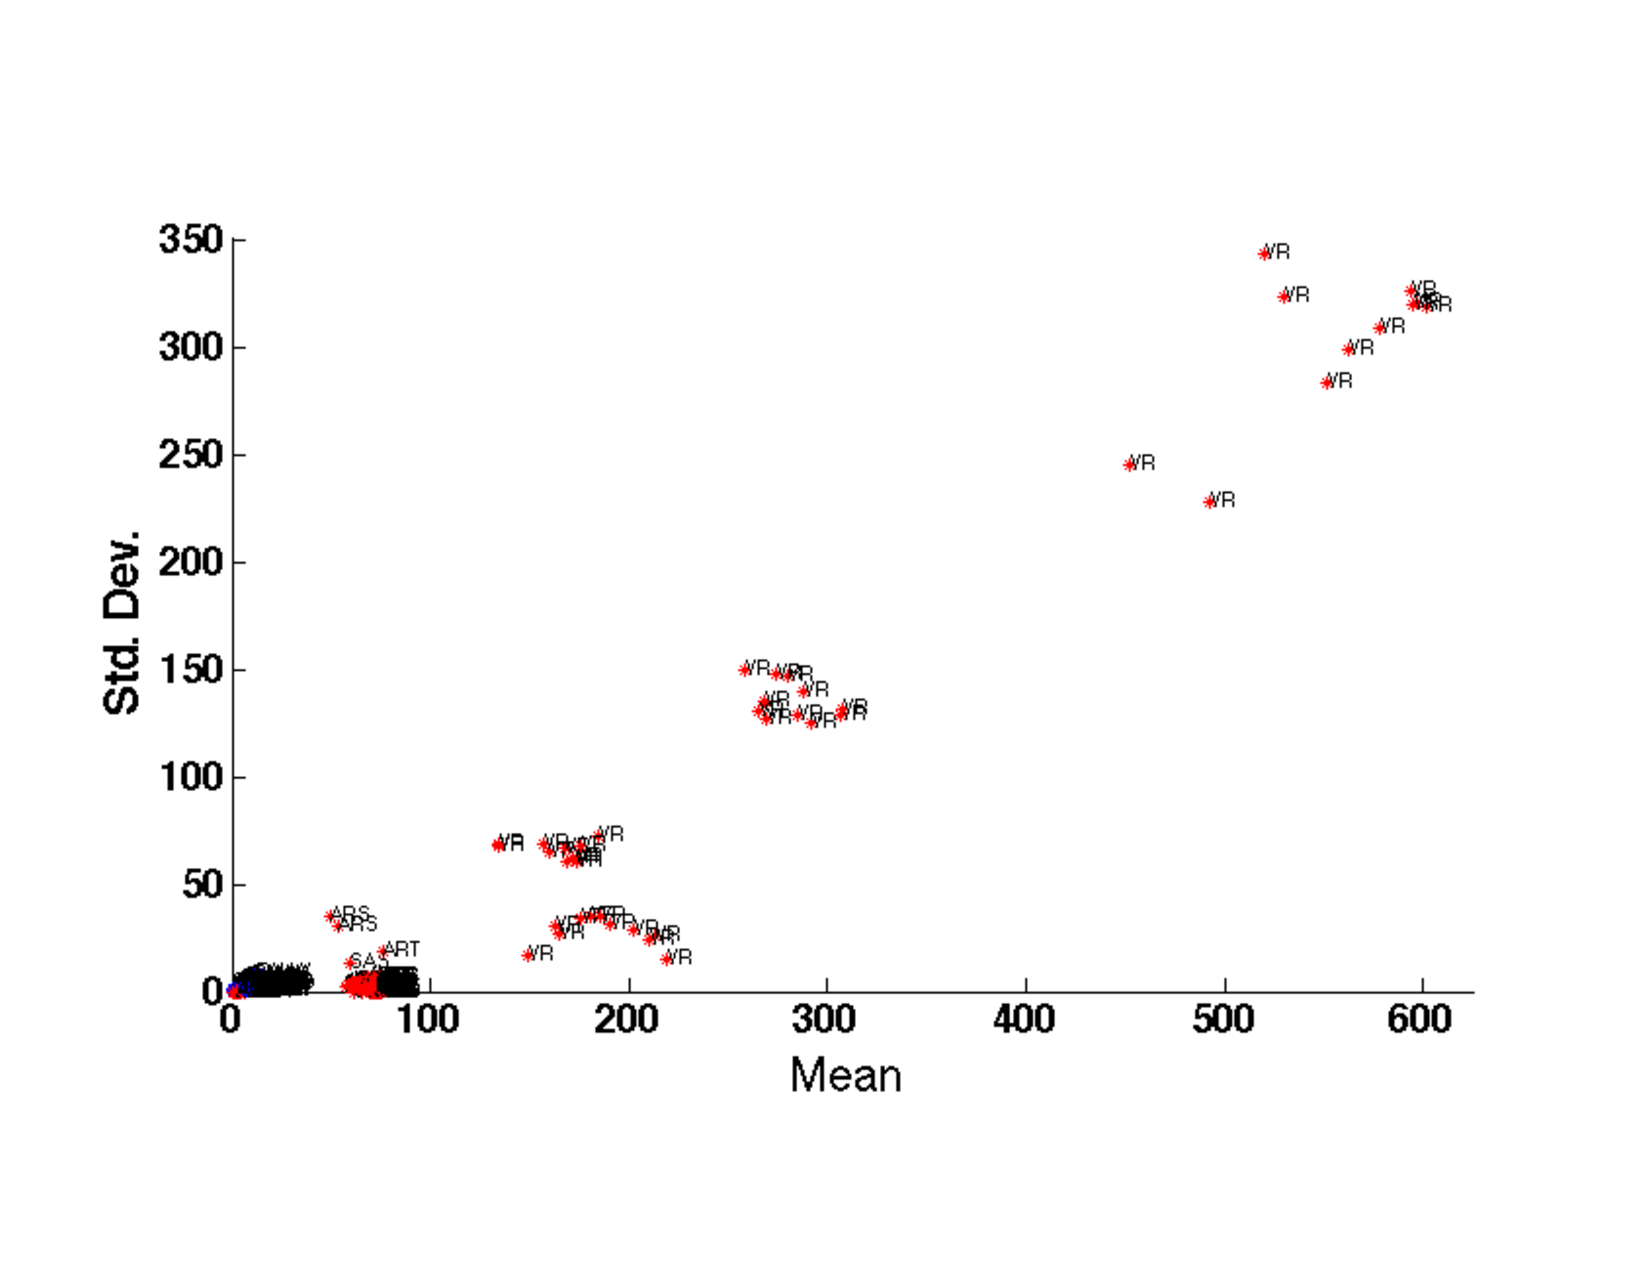
\includegraphics[width=1.0\columnwidth]{figs/VR}
\caption{}
\label{fig:tstreams}
\end{figure}

\begin{figure}[t!] %htbp
\centering
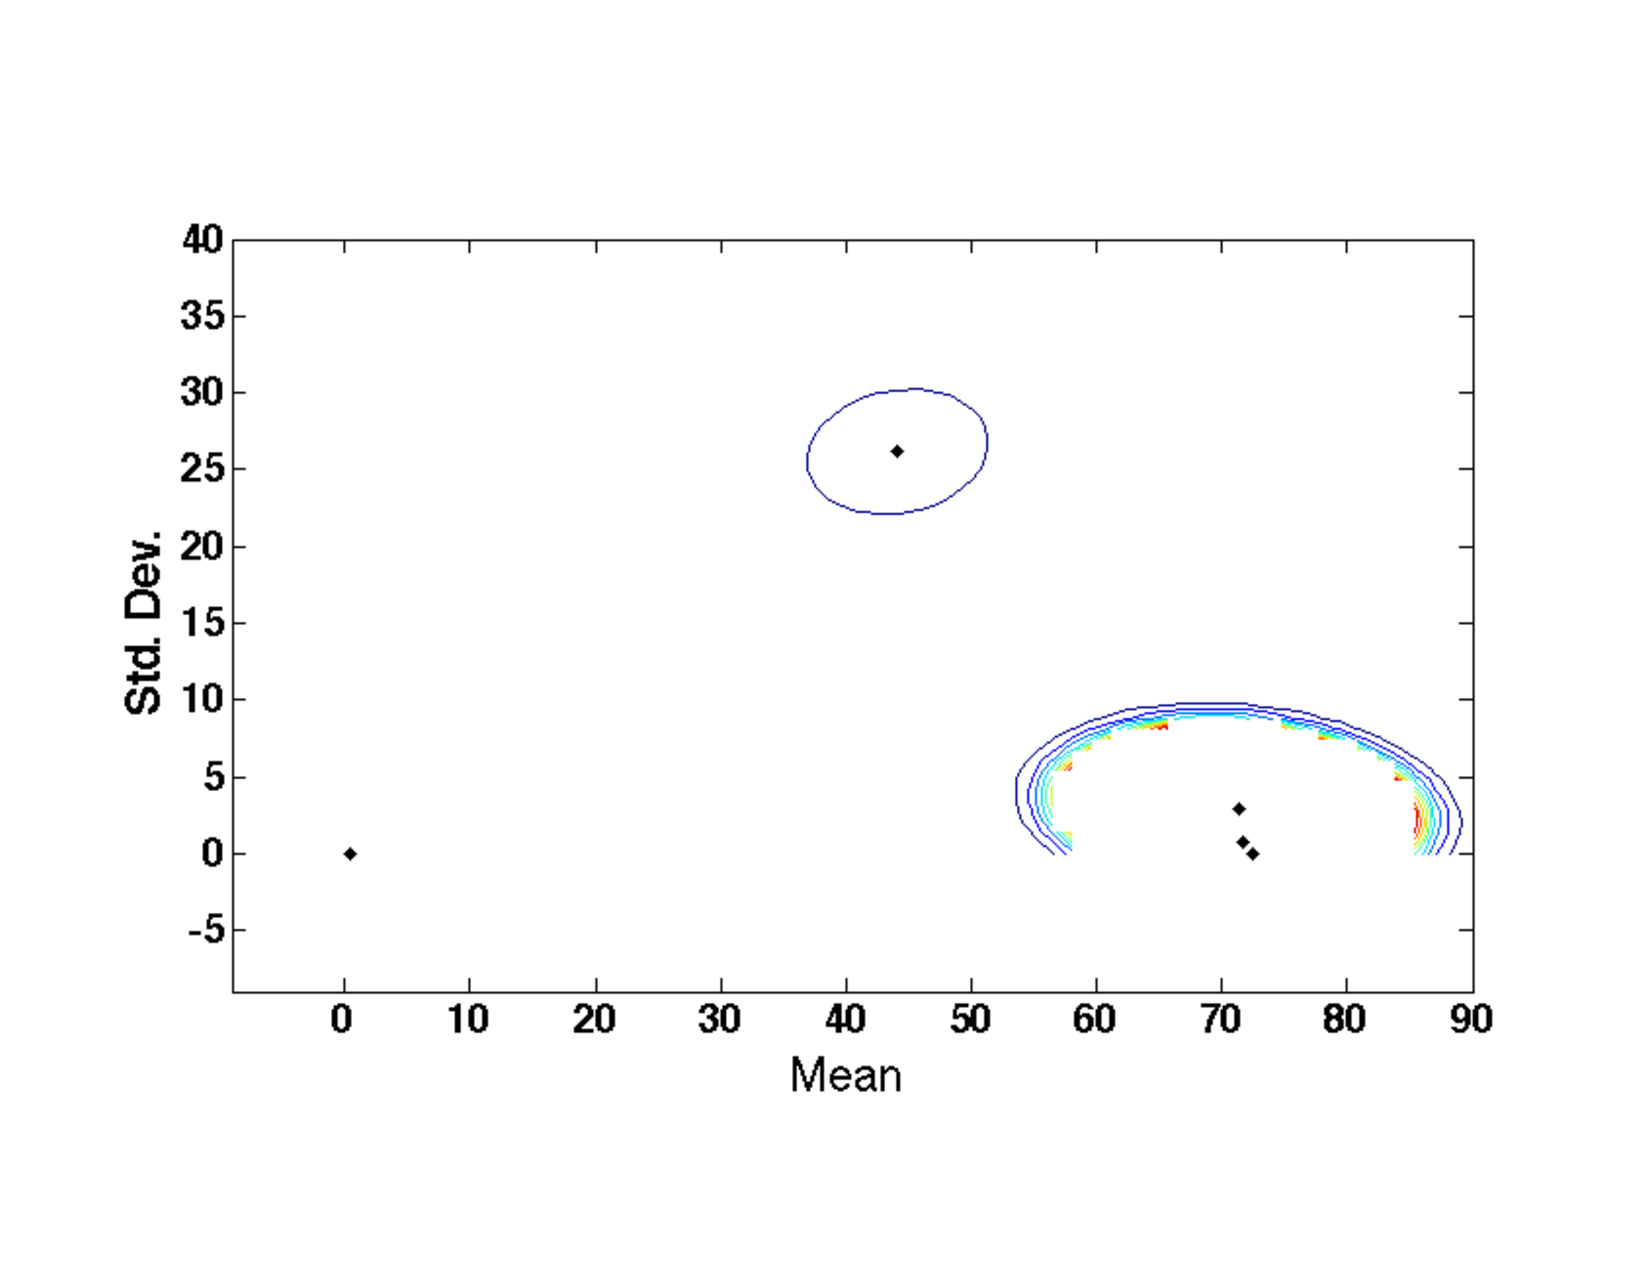
\includegraphics[width=1.0\columnwidth]{figs/gmm_centers}
\caption{}
\label{fig:tstreams}
\end{figure}


% \section{Value-Based Verification Through Physical-Model Checking}
\section{Related Work}
\section{Related work}

%\begin{itemize}
% \item dashboard
% \item andrew's lightin control work
% \item Kamin's hvac control work
% \item BEMs
% \item sMAP stuff
%\item Buildsys 2010 work~\cite{hbci}
%\item distributed consistency management: COPS
%\item mobility: tracking things with RFID~\cite{rfid_gonz2006}
%\item mobility: tracking of people, wifi indoor localization
%\item entity-relationship graphs
%\item homeOS [microsoft]
%\item HP Cooltown~\cite{cooltown}
%\end{itemize}
Our work touches on several areas from smart home research to logistics.  In the building space, there has been
some interest in building various kinds of energy-related visual and control applications.
This work focuses on the object definition, tracking, and management component of the architecture proposed by 
Hsu et al.~\cite{hbci}.  Their work stratefied the set of challenges that one could potentially face if the application 
were deployed at scale.  Our
work, in constrast, bases its design rationale on a \emph{real deployment} that is taking place at scale in a building 
on our campus.  We focus on solving fundamental systems challenges in dealing with intermittent connectivity
and conflict resolution in tracking people and things over time.  We also focus on leveraging gestures to minimize
the cost of interaction for users, while maximizing the information we can attain about the state of the world.

% Tracking people/indoor localization
An important aspect of the Energy Lens is determining when people and things have moved.  This requires some form 
of indoor localization.  There's a large body of literature in the area of indoor localization with mobile phones ranging from 
using wifi~\cite{radar}, to sonar~\cite{cricket}, to ambient noise~\cite{abs}, and a combination of sensors on the 
phone~\cite{surroundsense, darwinphone}.  Dita~\cite{dita} uses acoustic localization of mobile phones and also uses the infrastructure 
to determine gestures in free-space that are classified into pre-defined control actions.  Each of these require relatively complex 
software and/or infrastrure.  
We take a radically different, simple approach.  We use cheap, easy to re/produce tags (QR codes), place them on things in the 
environment over incrementally and use the natural \emph{swiping gesture} that users make, when interacting with the Energy Lens 
application, to track when they have moved or when the objects around them have moved.  The working principal is to attain as much 
information from their gesture to determine when something/one has moved.  We discuss our heuristics in section~\ref{sec:swipes}.

% context-aware apps
ACE~\cite{ACE} uses various sensors on the phone to infer a user's context.  The context domain consists of a set of user activities
and semantic locations.  For example, if ACE can distinguish between {\tt Running, Driving, AtHome, or InOffice}.  ACE also infers 
the one from the others, so if the user is {\tt AtHome} then they are not {\tt InOffice}.  Energy Lens uses inference to determine
when a person or thing has moved.  Certain swipe combinations give us information about whether they moved and where they moved to or
whether an item moved and where it moved to.  The main difference is that we only infer context when a user is actively swiping, rather
than a continuous approach.  Pretching is a fundamental technique used in many domains.  However, the cost of a prefetch for mobile
application outways the benefits if the prefetched data is not useful.  Informed mobile pretching~\cite{IMP} uses cost-benefit analysis 
to determine when to prefetch content for the user.  In the Energy Lens context, we prefetch data based on their location swipes.
We also rely on pretching to anticipate loss of connectivity, not just to improve preformance.

% Tracking things
Logistic systems focus on the tracking of objects as the move through distribution sites to warehouses, stores, shelves,
and purchase.  Items are tracked through bar code or RFID readers.  However, the workload is very structured and well
defined.  The authors of~\cite{rfid_gonz2006} describe this structure and leverage it to minimize storage
requirements and optimize query-processing performance.  Energy Lens uses the QR codes as the tag and the phone as an active
reader.  As objects move, users scan those items to their new location.  However, objects may belong to one or
many people, they can be metered by multiple meters a day, and their history in the system
is on-going.  In contrast, a typical logistics workload has a start (distribution site) and end point (leaving the store
after a sale).  In our workload, relationship semantics are important; we need to know whether the meter is \emph{bound-to}
rather than simple \emph{attached-to} an item.  We discuss the difference later in the paper.
% In addition to traditional logistics-style queries -- \emph{What is the average time that it took coffee-makers to move from the 
% warehouse to the shelf and finally to the checkout counter in January of 2004?} -- energy-analytics requires queries to group
% partial traces from meter data by tracking what meters the item attached to over the specified time-frame.
% The Energy Lens system collects and manages this kind of information to enable such queries.
Furthermore, we take advatange of natural gestures the user makes with the phone while scanning QR codes to extract
information about the current location of the user or things.

% Tagging items, virtual services
The key idea in the HP Cooltown~\cite{bridgingphysical,cooltown} work is to web-enable `things' in the world, grouped-by
`place', and accessed by `people' via a standardized acquisition protocol (HTTP) and format (HTML, XML).  
Cooltown creates a web presence for things in the world either directly (embedded web server) or indirectly 
(URL-lookup tag) as a web page page that display the services it provides.  Many of the core concepts in Cooltown 
also show up in Energy Lens.  The main overlap is the use of tags in the world that contain a reference to a virtual 
resource, accessible via HTTP through
a network connection.  Cooltown, however, explicitly chooses not maintain a centralized relationship
graph, it leverages the decentralized, linking structure of the web to group associated web pages together.
Furthermore, things are assumed to not move.  People are the main mobile entities.  The kind of applications
we wish to support must track where things are and their specific inter-relationships.  We imposed a richer set of 
semantics on our, centrally maintained, relationship graph and use it to provide detailed energy information.


\subsection{Related work}
The research community has addressed the detection of abnormal energy-consumption in buildings in numerous ways \cite{katipamula:1review2005,katipamula:2review2005}.
% Detecting abnormal energy-consumption in buildings has recently received the attention of the research community and different approaches have been studied.
% 

The rule-based techniques rely on a priori knowledge, they assert the sustainability of a system by identifying a set of undesired behaviors.
Using a hierarchical set of rules, Schein et al.\ propose a method to diagnose HVAC systems \cite{schein:hvacr2006}.
In comparison, state machine models take advantage of historical training data and domain knowledge to learn the states and transitions of a system.
The transitions are based on measured stimuli identified through a domain expertise.
State machines can model the operation of HVAC systems \cite{patnaik:toist2011} and permit to predict or detect the abnormal behavior of HVAC's components \cite{bellala:buildsys2012}.
However, the deployment of these methods require expert knowledge and are mostly applied to HVAC systems.

In~\cite{seem:energybldg2007}, the authors propose a simple unsupervised approach to monitor the average and peak daily consumption of a building and uncover outlier, nevertheless, the misbehaving devices are left unidentified.

Using regression analysis and weather variables the devices energy-consumption is predicted and abnormal usage is highlighted.
The authors of~\cite{brown:buildperf2012} use kernel regression to forecast device consumption and devices that behave differently from the predictions are reported as anomalous.
Regression models are also used with performances indices to monitor the HVAC's components and identify inefficiencies \cite{zhou:wiley2009}.
The implementation of these approaches in real situations is difficult, since it requires a training dataset and non-trivial 
parameter tuning.

Similar to our approach, previous studies identify abnormal energy-consumption using frequency analysis and unsupervised anomaly detection methods.
The device's consumption is decomposed using Fourier transform and outlier values are detected using clustering 
techniques \cite{Bellala_buildsys11,wrinch:pes2012,chen:aaaiw2011}. %jakkula
However, these methods assume a constant periodicity in the data and this causes many false positives in alarm reporting.  %, thus, they report devices usages happening at unusual times although they may not correspond to a faulty operation.
We do not make any assumption about the device usage schedule.  We only observe and model device relationships.
We take advantage of a recent frequency analysis technique that enables us uncover the inter-device relationships~\cite{romain:iotapp12}.
The identified anomalies correspond to devices that deviate from their normal relationship to other devices.

Reducing a building's energy consumption has also received a lot of attention from the research community.
% Since HVACs are one of the major electricity consumer in the buildings, several researchers have mainly focused on reducing the consumption of HVACs.
The most promising techniques are based on occupancy model predictions as they ensure that empty rooms are not over conditioned needlessly.
Room occupancy is usually monitored through sensor networks \cite{agarwal:ipsn2011,erickson:ipsn2011} or the computer network traffic \cite{kim:buildsys2010}.
These approaches are highly effective for buildings that have rarely-occupied rooms (e.g. conference room) and studies show that such approaches
 can achieve up to 42\% annual energy saving.
% However, these occupancy model predictions track human activity through sensor networks that usually imply the extra cost and privacy concerns.
SBS is fundamentally different from these approaches.  SBS identifies the abnormal usage of any devices rather than optimizing the normal usage of specific devices.
Nevertheless, the two approaches are complementary and energy-efficient buildings should take advantage of the synergy between them.






% Therefore, it is a practical way of reducing the energy consumption of any building in contrast to the anomaly detectors based on neural networks or kernel regression that requires training datasets and complex parameter tuning \cite{brown:buildperf2012}.
% Also, the proposed method does not require extra deployments such as sensors monitoring the room occupancy \cite{agarwal:ipsn2011,erickson:ipsn2011} or extra measurements for occupancy models (e.g. network traffic).
% 
% 
% This approach provides new insights in buildings energy consumption as it is fundamentally different from past works.
% complementary to other methods decreasing the energy consumption of the building normal operations.
% 
% it is more general (not only HVAC)
% 
% TODO look at IPSN TPC papers. Andreas Krause?

% 
% problem:
% The building energy consumption is mainly driven by its occupancy.
% The human occupancy is responsible for the majority of the devices energy consumption.
% For example, workstations, lights and air conditioners are utilized the most when humans occupied the building.
% 
% Thereby, all devices follow the same trend which is conducted by the human occupancy.
% In practice sensors data look all same.
% All devices are used during office hours and left off at night. (TODO see figure...)
% For our purpose, finding devices used simultaneously, this data is really difficult to analyze as the differences between each device is insignificant.
% 
% Our approach consists of; (1) subtract from the data the general trend driven by the building occupancy, (2) analyze remaining data to cluster devices used in concert.
% 
% 
% 
% result summary:
% We evaluate the proposed correlation estimator using 10 weeks of data from 135 devices serving 231 rooms.
% 
% contributions
% and advantages: unsupervised approach, small number of parameter (only one!), no training data required, no need of occupancy model/instrumentation, No distinction of weekdays, weekend, holidays...
% 
\subsection{Spatial Verifiction: Related Work}
There has been much research work on sensor stream clustering and trace analysis. Chen and Tu~\cite{DStream} investigate 
how to cluster data streams in real-time using a density-based approach with a two-tiered framework. The first tier captures 
the dynamics of a data stream with a density decaying technique and then maps it to a grid.  The second tier computes a grid 
density based on how it clusters the grid. Their approach differs from ours in that they focus on decreasing algorithm 
complexity for real-time sensor stream clustering.  We run our analysis on historical traces and use correlation analysis
in our clustering algorithm.

Kapitanova et al.~\cite{failure} describe a technique to monitor sensor operations in the home and identify sensor failures. 
The classifier is trained on historical sensor data to obtain the relationship between sensors, assuming the number and location of 
sensors is known.  When a failure or removal of a sensor occurs, the classifier's behavior deviates and the event is captured. Our method does not require any prior knowledge and instead tries to cluster feeds to discover their relative placement.

Lu and Whitehouse~\cite{blueprints} formulate a new algorithm, particularly leveraging the semantic constraints interpreted from sensor 
data to determine sensor locations. The algorithm identifies how many rooms are present using motion sensors and determines room position based on physical constraints. Finally, it maps each sensor into the associated room. Our efforts focus on using intrinsic patterns typically pre-existing in building system sensor feeds to uncover physical relationships.

Fontugne et al.~\cite{IOT} propose a new method to decompose sensor signals with EMD.
They extract the intrinsic usage pattern from the raw traces and show that sensors close to each other have higher intrinsic correlation. However, they do not explore the observation more deeply by answering whether there is a statistically discoverable boundary between sensor clusters in different rooms, or if there is a uniform threshold in the correlation coefficients able to be generalized to different rooms.

Fontugne et al.~\cite{SBS} carry on the work and propose an unsupervised method to monitor sensor behavior in buildings. They constructed 
a reference model out of the underlying pattens, obtained with EMD,  and use it to compare future activity against it.  They report an anomaly whenever a device deviates from the reference. This work exploits EMD as a method to detrend the signals and capture the inter-device relationships.

Much work utilizes EMD on medical data~\cite{ecg}, speech analysis~\cite{speech}, image processing~\cite{ip} 
and climate analysis~\cite{climate}. Our method adopts EMD to determine whether a discoverable statistical boundary exists in sensors traces
from sensors in different rooms and whether such a boundary
 can be generalized across rooms with various kinds of sensors.


\section{Summary}
\subsection{Limitations}
EMD is useful for finding underlying behavioral relationships between traces of sensor data.  However,
when we set the timescales smaller than a day, the results were not as strong.
The trace has to be long enough to capture the trend.  For this data set, the underlying
trend is daily, therefore it requires there to be a significant number of samples over many days.
%  to
% for this method to be effective.
Although this was a limitation for this dataset, it really depends on the underlying phenomenon that
the sensors are measuring.  Its underlying trend is ultimately what EMD will be able to separate
from the intrinsic modes of the underlying signal.

\subsection{Discussion}
EMD allows us to effectively identify fundamental relationships between sensor traces.
% Using EMD to find fundamental relationships between sensor traces effectively identifies intrinsically
% related behavioral relationships.
% was quite promising for building
% up models of correlated usage.  
We believe that identifying meaningful usage-correlation patterns can help reduce oversights
by the occupants and faults that lead to energy waste.  A direct application of this is the identification
of simultaneous heating and cooling~\cite{simheatcool}.  Simultaneous heating and cooling is when heating
and cooling system either compete with one another or compete with the incoming air from outside and is
a cause for major energy waste in building~\cite{simheatcool}.  The longer it goes undetected,
the more waste there is.  However, it is very difficult to identify since the occupants do not notice
changes in temperature.  Our analysis can be used to build a correlation model between the outside
heating cooling temperature, the cooling coil temperature, and the outside air vent position.  If their behavior
is not correlated as expect, an alarm should be raised.

We can also apply it to other usage scenarios.  In our traces, for example, we found an instance where the pump
was on, but the lights were off.  The two are typically correlated, however, in this case they were not.
The air conditioning was pumping cool air into a room without occupants.
With our approach this could have been identified and corrected.  In future work, we intend to
package our solution to serve these kinds of applications.

% EMD works perfectly although the weekly pattern of the data is altered the last analyzed week.

% EMD inherently finds the interesting time scales.

% number of zero crossing = mean frequency/time scale:
%   TODO give the time scale for each IMF.


\section{Conclusion}
% what is our problem

% what we did

% contributions and main results

% future work


This paper set out to examine the underlying relationship between sensor traces to find interesting correlations
in use.  We used data from a large deployment of sensors in a building and found that direct correlation analysis on the raw
traces was not discriminatory enough to find interesting relationships.  Upon closer inspection, we noticed that
the underlying trend was dominating the correlation calculation.  In order to extract meaningful behavior this trend has
to be removed.  We concluded that empirical mode decomposition is a helpful analytical tool for de-trending 
non-linear, non-stationary data; inherent attributes contained by our traces.

We re-ran our analysis on the same traces, except we correlated the IMF outputs of the EMD operation on each of the traces and found that the pump was closely related to the lights in the same room served by the pump and
uncorrelated with a pump on the same floor serving a different room.  In order to corroborate the applicability
of our approach, we compared the pump trace with \emph{all} 674 sensor traces and found a strong correlation
between the relative spatial position of the sensors and their IMF correlations.  The most correlated IMFs were 
serving the same
area in the building.  As we relax the admittance criteria we find that the spatial correlation expands radially from
the main location served by the reference trace.

We plan to examine the use of this method in applications that help discovery changes in underlying relationships over time
in order to identify opportunities for savings in buildings.  We will use it to build inter-device correlation models
and use these models to establish ``normal'', ``abnormal'' usage patterns.  We hope to take it a step further and include a
supervised learning approach to distinguish between ``efficient'' and ``inefficient'' usage patterns as well.







\section{Discussion} \label{discussion}
%The additional advantages of SBS are discussed in this section.
%practical
SBS is a practical method for mining device traces, uncovering hidden relationships and abnormal behavior. 
In this paper, we validate the efficacy of SBS using the sensor metadata (i.e. device types and location), however, these 
tags are not needed by SBS to uncover devices relationships.
Furthermore, SBS requires no prior knowledge about the building and deploying our tool to other buildings requires no human intervention --
neither extra sensors nor a training dataset is needed. 

%best effort
SBS is a best effort approach that takes advantage of all the existing building sensors.
For example, our experiments revealed that SBS indirectly uncovers building occupancy through device use (e.g. the elevator in the Building 2). 
The proposed method would benefit from existing sensors that monitor room occupancy as well (e.g. those deployed in~\cite{agarwal:ipsn2011,erickson:ipsn2011}).  % albeit they are no needed.
Savings opportunities are also observable with a minimum of 2 monitored devices and building energy consumption can be better understood after using SBS.

% good=bad..
SBS constructs a model for normal inter-device behavior by looking at the usage patterns over time, thus, we run the risk that
a device that constantly misbehaves is labeled as normal.  % is considered as normal by SBS.
Nevertheless, building operators are able to quickly identify such perpetual anomalies by validating the clusters of correlated devices uncovered by SBS.
The inspection of these clusters is effortless compare to the investigation of the numerous raw traces.  
Although this kind of scenario is possible it was not observed in our experiments.
%Note, that this type of anomaly is unseen in our experiments and is expected to be rare.

%EMD
%Striping sensor data with EMD is beneficial for other work.
In this paper, we analyze only the data at medium frequencies, however, we observe that data at the high frequencies and residual data (Figure \ref{fig:heatmap}) also permits us to determine the device type.  % as well.
This information is valuable to automatically retrieve and validate device labels -- a major challenge in building metadata
management.

% future work
This paper aims to establish a methodology to identify abnormalities in device power traces and inter-device usage patterns.
In addition, we are planning to apply this method to online detection using, for example, a sliding window to compute an adaptive reference matrix that evolve in time.
However, designing such system raises new challenges that are left for future work.

% %limitation
% The goal of this article is to develop an unsupervised tool that identifies energy wastes in buildings.
% However, the design of the system that reports these energy waste in real time is beyond the goal of this work.
% more work is needed to allow on line detection: use of smaller time bin.
% 
% 
% season changes; devices relationships have seasonal pattern thus we may need forecast models such as ARIMA to make the reference matrix evolve in time.

\section{Conclusions}
The goal of this article is to assist building administrators in identifying misbehaving devices in large building sensor
deployments.  
We proposed an unsupervised method to systematically detect abnormal energy consumption in buildings: the Strip, Bind, and Search (SBS) method.
SBS uncovers inter-device usage patterns by striping dominant trends off the devices energy-consumption trace.
Then, it monitors device usage and reports devices that deviate from the norm.  
Our main contribution is to develop an unsupervised technique to uncover the true inter-device relationships that are hidden by noise and 
dominant trends inherent to the sensor data.  
SBS is used on two sets of traces captured from two buildings with fundamentally different infrastructures.
The abnormal consumption identified in these two buildings are mainly energy waste.
The most important one is an instance of a competing heater and cooler that caused the heater to waste around 2500~kWh.



\section*{Acknowledgments}
The authors thank Hideya Ochiai for providing the data from the University of Tokyo.
This research was partially supported by the JSPS fellowship program and the CNRS/JSPS Joint Research Project.
This work is also supported in part by the National Science Foundation under grants CPS-0932209 and CPS-0931843.




